\documentclass[a4paper,10pt
,draft
]{article}%


\usepackage[hidelinks]{hyperref}
\hypersetup{
  % colorlinks,
  final,
  pdftitle={Equivariant Dendroidal Segal Spaces},
  pdfauthor={Bonventre, P. and Pereira, L. A.},
  % pdfsubject={Your subject here},
  % pdfkeywords={keyword1, keyword2},
  linktoc=page
}
\usepackage[open=false]{bookmark}


\input{commands.tex}%




%-------- TIKZ -----------------------------------------
\usepackage{tikz}%
\usetikzlibrary{matrix,arrows,decorations.pathmorphing,
cd,patterns,calc}
\tikzset{%
  treenode/.style = {shape=rectangle, rounded corners,%
                     draw, align=center,%
                     top color=white, bottom color=blue!20},%
  root/.style     = {treenode, font=\Large, bottom color=red!30},%
  env/.style      = {treenode, font=\ttfamily\normalsize},%
  dummy/.style    = {circle,draw,inner sep=0pt,minimum size=2mm}%
}%

\usetikzlibrary[decorations.pathreplacing]
% \usetikzlibrary{external}\tikzexternalize
% \makeatletters
% \renewcommand{\todo}[2][]{\tikzexternaldisable\@todo[#1]{#2}\tikzexternalenable}
% \makeatother


% -------- COMMANDS ON DRAFT--------------------------

\usepackage{ifdraft}
\ifdraft{
  \color[RGB]{63,63,63}
  % \pagecolor[rgb]{0.5,0.5,0.5}
  \pagecolor[RGB]{220,220,204}
  % \color[rgb]{1,1,1}
}

\usepackage[draft]{showkeys}
\usepackage{todonotes}%[obeyDraft]


% -------- Reference Numbering
% \numberwithin{equation}{section}%
% \numberwithin{figure}{section} 


% ------- Author Info -----------------------

\author{Peter Bonventre, Lu\'is A. Pereira}%
\title{Equivariant dendroidal Segal spaces and $G$-$\infty$-operads}%
\date{\today}



%----- Document ---------------------------------



\begin{document}	\maketitle%



\begin{abstract}
      bla bla, generalizing \cite{CM13a}.
      
      In an appendix, we discuss Reedy categories in the equivariant context.
\end{abstract}



\tableofcontents


%\section{Overview}
%
%The following are the categories currently with model structures and the right adjoints of already established Quillen equivalences.
%\[
%	\begin{tikzcd}
%		\mathsf{PreOp}^G
%\\
%		\mathsf{sdSet}^G \ar{r}[swap]{(-)_0} \ar{u}{\gamma_{\**}} &
%		\mathsf{dSet}^G
%	\end{tikzcd}
%\]
 


\section{Introduction}

This paper follows \cite{Per17} and \cite{BP17} and is the third piece of a larger project aimed at understanding the homotopy theory of 
\textit{equivariant operads with norm maps}.
Informally, norm maps are a new piece of structure that must be considered when dealing with equivariant operads
(and which has no analogue in the theory of equivariant categories).
The need to understand norm maps, particularly in the context of $G$-ring spectra,
as well as their usefulness,
was made clear by Hill, Hopkins and Ravenel in their solution of the Kervaire invariant one problem \cite{HHR16}.

The starting point of this project was the discovery by the authors of,
for each finite group $G$,
a category $\Omega_G$ of $G$-trees whose objects diagrammatically encode compositions of norms maps 
and whose arrows encode the necessary compatibilities between such compositions.
Our categories $\Omega_G$ are a somewhat non-obvious equivariant generalization of the dendroidal category $\Omega$
of Cisinski-Moerdijk-Weiss, 
and indeed all the key combinatorial concepts in their work,
such as faces, degeneracies, boundaries and horns, generalize to $G$-trees \cite[\S 5,6]{Per17}.
As such, it is natural to ask whether the Cisinski-Moerdijk program \cite{CM11},\cite{CM13a},\cite{CM13b} can also be generalized to the equivariant context. 

We recall that the main result of their program is the existence of a Quillen equivalence
\[
	W_{!} \colon \mathsf{dSet} 
		\rightleftarrows
	\mathsf{sOp}  \colon N_{hc} 
\]
where $\mathsf{dSet} = \mathsf{Set}^{\Omega^{op}} $
is the category of presheaves over $\Omega$, 
called \textit{dendroidal sets},
and 
$\mathsf{sOp}$ is the category of simplicial colored operads.
Their program was carried out in three main steps:
\begin{inparaenum}
	\item[(i)] \cite{CM11} established the existence of the model structure on $\mathsf{dSet}$
	(with some of the key combinatorial analysis based on Moerdijk and Weiss' work in \cite{MW09});
	\item[(ii)] \cite{CM13a} established auxiliary model structures on the categories $\mathsf{sdSet}$ and $\mathsf{PreOp}$
	of dendroidal spaces and pre-operads, and showed that all three of $\mathsf{dSet}$, $\mathsf{sdSet}$ and $\mathsf{PreOp}$ are Quillen equivalent;
	\item[(iii)] lastly, \cite{CM13b} established the existence of the model structure on $\mathsf{sOp}$ as well as the Quillen equivalence between $\mathsf{sOp}$ and $\mathsf{PreOp}$, finishing the proof of the main result.
\end{inparaenum}

From the perspective of the Cisinski-Moerdijk program, 
\cite{Per17} is then the equivariant analogue of the first step \cite{CM11} (as well as \cite{MW09}), 
while the present paper provides the equivariant analogue of the
second step \cite{CM13b}.
More explicitly, in \cite{Per17}, and inspired by the category $\Omega_G$ of $G$-trees,
the second author equipped the category
$\mathsf{dSet}^G$ of $G$-equivariant dendroidal sets with a model structure whose fibrant objects 
are ``equivariant operads with norm maps up to homotopy'',
called $G$-$\infty$-operads.
Further, it was shown therein that whenever a $G$-operad
$\O \in \mathsf{sOp}^G$ is
suitably fibrant the homotopy coherent nerve
$N_{hc}(\O)$ is such a 
$G$-$\infty$-operad (rather than just an ``$\infty$-operad with $G$-action'').
In the present paper, our main results are then the existence of suitable model structures on the categories 
$\mathsf{sdSet}^G$ and $\mathsf{PreOp}^G$
of $G$-dendroidal spaces and $G$-pre-operads,
as well as the existence of Quillen equivalences
between all three of 
$\mathsf{dSet}^G$, $\mathsf{sdSet}^G$ and $\mathsf{PreOp}^G$.

It is worth noting that, much as was the case with the work in \cite{Per17}, our results are not formal consequences of their non-equivariant analogues, due to the nature of norm maps\footnote{Recall that by using the inclusions of simplicial categories and simplicial sets into simplicial operads and dendroidal sets (cf. the introduction to \cite{CM13b}), the Cisinski-Moerdijk program recovers the Bergner-Joyal-Lurie-Rezk-Tierney program studying $\infty$-categories. As a point of contrast, we note that the lack of norms in the categorical case causes the equivariant generalization of this latter program to indeed be formal; see \cite{Ste16,Ber17}.}.
Indeed, in \cite{BP17}, the second piece of our project,
the authors introduced the notion of 
\textit{genuine equivariant operads},
which are new algebraic objects motivated by the combinatorics of norm maps as encoded by the category $\Omega_G$ of $G$-trees.
And while a priori the work in \cite{BP17} is largely perpendicular to the Cisinski-Moerdijk program
(the main result \cite[Thm. III]{BP17} is what one might call the 
``operadic Elmendorf-Piacenza theorem'', which is an equivariant phenomenon),
many of the new technical hurdles in this paper versus \cite{CM13a} can be traced back to the fact that
at many points in the discussion we are secretly dealing with colored genuine equivariant operads, 
which are the colored generalization of the structures discussed in \cite{BP17},
and the formal definition of which we prefer to postpone to a follow-up paper.

\vskip 10pt

The organization of the paper is as follows.

{\color{blue} Fill this}


\section{Preliminaries}

\subsection{The category of trees $\Omega$}

We start by recalling the key features of the category $\Omega$ of trees that will be used throughout.
Our official model for $\Omega$ will be Weiss' algebraic model of \textit{broad posets} as discussed in \cite[\S 5]{Per17},
% and \cite{Wei12},
hence we first recall some key notation and terminology.
Given a tree diagram $T$ such as
\begin{equation}\label{FIRSTTREE EQ}
	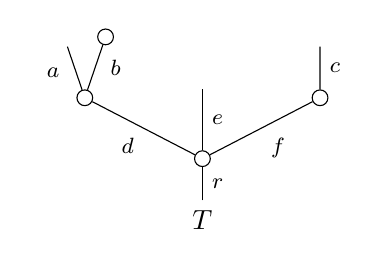
\begin{tikzpicture}[auto,grow=up,
	level distance = 2.2em,
	every node/.style={font=\footnotesize,minimum size=1.5mm}]%
	\tikzstyle{level 2}=[sibling distance=4.25em]%
	\tikzstyle{level 3}=[sibling distance=1.5em]%
		\node at (0,0)[font=\normalsize]{$T$}%
			child{node [dummy] {}%
				child{node [dummy] {}%
					child{node {}%
					edge from parent node [swap] {$c$}}%
				edge from parent node [swap] {$f$}}%
				child[level distance = 2.5em]{
				edge from parent node [swap] {$e$}}%
				child{node [dummy] {}%
					child{node[dummy] {}%
					edge from parent node [very near end,swap] {$b$}}%
					child{node {}%
					edge from parent node [very near end] {$\phantom{b}a$}}%
				edge from parent node {$d$}}%
			edge from parent node [swap] {$r$}};%
	\end{tikzpicture}%
\end{equation}
and for each edge $t$ of $T$ topped by a vertex $\circ$, 
we write $t^{\uparrow}$ to denote the tuple of edges immediately above $t$.
In our example, 
$r^{\uparrow}=def$, 
$d^{\uparrow} = ab$,
$f^{\uparrow} = c$ and
$b^{\uparrow} = \epsilon$, 
where $\epsilon$ is the empty tuple.
Edges $t$ for which:
\begin{inparaenum}
\item[(i)] $t^{\uparrow} \neq \epsilon$, such as $r,d,f$, are called \textit{nodes};
\item[(ii)] $t^{\uparrow} = \epsilon$, such as $b$, are called \textit{stumps};
\item[(iii)] $t^{\uparrow}$ is undefined, such as $a,c,e$, are called \textit{leaves}.
\end{inparaenum}
The vertices of $T$ are then encoded symbolically as 
$t^{\uparrow} \leq t$, which we call a \textit{generating broad relation}. 
This notation is meant to suggest a form of transitivity: for example, the generating relations
$ab \leq d$ and $def \leq r$
generate, via \textit{broad transitivity},
a relation $abef \leq r$
(we note that this is essentially compact notation for the operations and composition in the colored operad generated by $T$
\cite[\S 3]{MW07}). The other broad relations obtained by broad transitivity are 
$dec \leq r$,
$abec \leq r$,
$aec \leq r$,
$a \leq d$.
The set of edges of $T$ together with these broad relations
(as well as identity relations $t \leq t$) form the 
\textit{broad poset} associated to the tree, which is again denoted $T$.

Given a broad relation $t_0 \cdots t_n \leq t$,
we further write $t_i \leq_d t$.
Pictorially, this says that the edge $t_i$ is above $t$,
and it is thus clear that $\leq_d$ defines a partial order on edges of $T$.
Trees always have a single $\leq_d$-maximal edge, called the \textit{root}. Edges other than the root or the leaves are called \textit{inner edges}. In our example $r$ is the root, $b,d,f$ are inner edges and $a,e,c$ are leaves. 

We denote the sets of edges (inner edges, vertices) of $T$ by
$E(T)$ (resp. $E^{\mathsf{i}}(T)$, $V(T)$).

The Cisinski-Moerdijk-Weiss category $\Omega$ of trees then has as objects tree diagrams as in \eqref{FIRSTTREE EQ}
and as maps $\varphi \colon T \to S$ the monotone maps of broad posets
(meaning that if $t_1 \cdots t_k \leq t$ then
$\varphi(t_1) \cdots \varphi(t_k) \leq \varphi(t)$).
In fact, Weiss further identified axioms characterizing those broad posets that are associated to trees (see \cite[Defs. 5.1 and 5.9]{Per17}).

Further, our discussion will be somewhat simplified by the assumption that $\Omega$
contains exactly one representative of each planarized tree.
Informally, this means that trees $T \in \Omega$
come with a preferred planar representation,
though this can also be formalized in purely algebraic terms, see \cite[\S 3.1]{BP17}.
For our purposes, the main consequence is that any map 
$S \to T$ in $\Omega$ has a (strictly) unique factorization
$S \simeq S' \to T$ as an isomorphism followed by a \textit{planar map} \cite[Prop. 3.21]{BP17}. 
Roughly speaking, $S'$ is obtained from $S$
by pulling back the planarization of $T$.

We now recall the key classes of maps of $\Omega$.
A map $\varphi \colon S \to T$ which is injective on edges is called a \textit{face map}
while a map that is surjective on edges and preserves leaves is called a \textit{degeneracy map}
(the extra requirement ensures that leaves of $S$ do not become stumps of $T$).
Moreover, a face map is further called an \textit{inner face map}
if $\varphi(r_S) = r_T$ and 
$\varphi(\underline{l}_S) = \underline{l}_T$ 
(where $r_{(-)}$ denotes the root edge and $\underline{l}_{(-)}$ the leaf tuple)
and called an \textit{outer face map} if it does not factor through any non-identity inner face maps.
The following result is \cite[Cor. 3.32]{BP17}.
\begin{proposition}\label{UNIQUEFACT PROP}
	A map $\varphi \colon S \to T$ in $\Omega$ has a factorization, unique up to unique isomorphisms,
\[
	S \xrightarrow{\varphi^{-}}
	U \xrightarrow{\varphi^{i}}
	V \xrightarrow{\varphi^{o}}
	T	
\]
as a degeneracy followed by an inner face map followed by an outer face map.
\end{proposition}

We now recall a more explicit characterization (and notation) for planar inner/outer faces
(planar degeneracies are characterized by edge multiplicities, see \cite[Prop. 3.47(ii)]{BP17}).
For any subset $D \subseteq E(T)$, there is a planar inner face
$T-D$ which removes the inner edges in $E$ but keeps all broad relations involving edges not in $D$
(this is the hardest class of maps to visualize pictorially, as the vertices adjacent to each $d \in D$ are combined via broad transitivity/composition).
For each broad relation
$t_1 \cdots t_k = \underline{t} \leq t$ in $T$,
there is a planar outer face
$T_{\underline{t} \leq t}$
such that
$r_{T_{\underline{t} \leq t}} = t$ and
$\underline{l}_{T_{\underline{t} \leq t}} = \underline{t}$
(in fact, by Proposition \ref{UNIQUEFACT PROP} this is the maximal such face).
Moreover, the edges $s$ of $T_{\underline{t} \leq t}$ are the edges of $T$ such that
$s \leq_d t$ and $\forall_{i} s \not < t_i$ while the vertices are the $s^{\uparrow} \leq s$ such that 
$s \leq_d t$ and $\forall_{i} s \not \leq t_i$ 
(pictorially, $T_{\underline{t} \leq t}$ removes the parts of $T$ not above $t$ and above some $t_i$).


\begin{remark}\label{INNFULL REM}
	Inner faces $T-D \hookrightarrow T$ are always full, i.e. $T-D$ contains all broad relations of $T$ whose edges are in $T-D$.
	By contrast, whenever $T$ has stumps some of its outer faces $T_{\underline{t} \leq t}$ are not full,
	the main example being the maximal outer faces
	``removing stumps'' \cite[Not. 5.41]{Per17}.
\end{remark}


\begin{remark}\label{DEGREE REM}
	Following \cite[Ex. 2.8]{BM11}, one has a degree function 
	$|-|\colon \Omega \to \mathbb{N}$ given by $|T|=|V(T)|$
	such that non isomorphim face maps (resp. degeneracies) strictly increase (decrease) $|-|$.
	The category of face maps is thus denoted $\Omega^+$ and that of degeneracies is denoted $\Omega^-$.
\end{remark}

We now collect a couple of useful lemmas concerning faces.

\begin{lemma}\label{INNINT LEM}
	Consider a diagram of planar faces in $\Omega$
	(implicitly regarded as inclusion maps)
\[
\begin{tikzcd}[column sep =3em]
	V \ar[hookrightarrow]{r}{\text{out}} 
	\ar[hookrightarrow]{d}[swap]{\text{inn}} &
	U \ar[hookrightarrow]{d}
\\
	\bar{V} \ar[hookrightarrow]{r}{\text{out}}&
	\bar{U}
\end{tikzcd}
\]
	such that the horizontal maps are outer face maps and the left vertical map is an inner face map.

Then $E^{\mathsf{i}}(V) = E^{\mathsf{i}}(U) \cap E^{\mathsf{i}} (\bar{V})$.
\end{lemma}

\begin{proof}
	Write $r$ and $\underline{l}=l_1\cdots l_n$
	for the root and leaf tuple of $V$, or equivalently $\bar{V}$.
	Since the horizontal maps are outer, an edge
	$e \in E^{\mathsf{i}}(U)$ (resp. $e \in E^{\mathsf{i}}(\bar{U})$)
	is also in $E^{\mathsf{i}}(V)$ (resp. in $E^{\mathsf{i}}(\bar{V})$) iff
	$e <_d r$ and $\forall_i e \not \leq l_i$.
	But then $E^{\mathsf{i}}(V) = E^{\mathsf{i}}(U) \cap E^{\mathsf{i}}(V) = E^{\mathsf{i}}(U) \cap E^{\mathsf{i}}(\bar{V})$. 
\end{proof}


\begin{lemma}\label{CUPCAP LEM}
	Let $\{U_i \hookrightarrow T\}$ be a collection of planar outer faces of $T$ with a common root $t$. Then there are planar outer faces
	$U^{\cup} \hookrightarrow T$, $U^{\cap} \hookrightarrow T$,
	also with root $t$, such that
\begin{equation}\label{CUPCAP EQ}
	E(U^{\cup}) = \bigcup_i E(U_i), \quad
	V(U^{\cup}) = \bigcup_i V(U_i), \qquad
	E(U^{\cap}) = \bigcap_i E(U_i), \quad
	V(U^{\cap}) = \bigcap_i V(U_i).
\end{equation}
Moreover, these are the smallest (resp. largest) outer faces
containing (contained in) all $U_i$.
\end{lemma}

\begin{remark}
	One can check that it actually suffices to assume the $U_i$ have a common edge.
\end{remark}

\begin{proof}
	\eqref{CUPCAP EQ} determines pre-broad posets 
	(cf. \cite[Rem. 5.2]{Per17}) $U^{\cup}$ and $U^{\cap}$,
	hence we need only verify the axioms in 
	\cite[Defs. 5.1, 5.3, 5.9]{Per17}. 
	Antisymmetry and simplicity are inherited from $T$, the nodal axiom is obvious from \eqref{CUPCAP EQ}, and the root axiom follows since the $U_i$ have a common root (in $U^{\cap}$ case note that if $s$ is in $U^{\cap}$, then so is any $s'$ such that
	$s \leq_d s' \leq_d t$).
\end{proof}



\subsection{The category of $G$-trees $\Omega_G$}

We next recall the category $\Omega_G$ of $G$-trees first defined in \cite[\S 5.3]{Per17}. We start with an explicit and representative example of a $G$-tree (for more examples, see \cite[\S 4.3]{Per17}).
Letting $G = \{ \pm 1, \pm i, \pm j, \pm k\}$ denote the group of quaternionic units 
and $G \geq H \geq K \geq L$ denote the subgroups %
$H = \langle j \rangle$, %
$K = \langle -1 \rangle$, %
$L = \{1\}$,
there is a $G$-tree $T$ with 
\textit{expanded representation}
given by the two trees on the left below and
\textit{orbital representation}
given by the (single) tree on the right.
\begin{equation}\label{TWOREP EQ}
	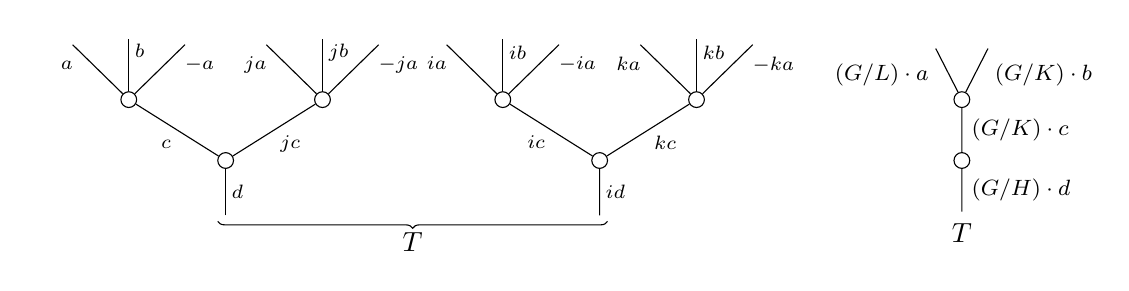
\begin{tikzpicture}[auto,grow=up, level distance = 2.2em,
	every node/.style={font=\scriptsize,inner sep = 2pt}]%
		\tikzstyle{level 2}=[sibling distance=7em]%
		\tikzstyle{level 3}=[sibling distance=2.25em]%
			\node at (4.75,0){}%	
				child{node [dummy] {}%
					child{node [dummy] {}%
						child{node {}%
						edge from parent node [swap,very near end] {$-k a$}}%
						child[level distance = 2.4em]{node {}%
						edge from parent node [swap,near end] {$k b$}}%
						child{node {}%
						edge from parent node [very near end] {$k a$}}%
					edge from parent node [swap] {$k c$}}%
					child{node [dummy] {}%
						child{node {}%
						edge from parent node [swap,very near end] {$-i a$}}%
						child[level distance = 2.4em]{node {}%
						edge from parent node [swap,near end] {$i b$}}%
						child{node {}%
						edge from parent node [very near end] {$i a$}}%
					edge from parent node  {$i c$}}%
				edge from parent node [swap] {$i d$}};%
			\node at (0,0){}%	
				child{node [dummy] {}%
					child{node [dummy] {}%
						child{node {}%
						edge from parent node [swap,very near end] {$-j a$}}%
						child[level distance = 2.4em]{node {}%
						edge from parent node [swap,near end] {$j b$}}%
						child{node {}%
						edge from parent node [very near end] {$j a$}}%
					edge from parent node [swap] {$j c$}}%
					child{node [dummy] {}%
						child{node {}%
						edge from parent node [swap,very near end] {$-a\phantom{j}$}}%
						child[level distance = 2.4em]{node {}%
						edge from parent node [swap,near end] {$b\phantom{j}$}}%
						child{node {}%
						edge from parent node [very near end] {$\phantom{-j}a$}}%
					edge from parent node  {$\phantom{j}c$}}%
				edge from parent node [swap] {$d$}};%
		\begin{scope}[every node/.style={font=\footnotesize}]%
			\node at (9.35,0){}%
				child{node [dummy] {}%
					child{node [dummy] {}%
						child{node {}%
						edge from parent node [swap,very near end] {$(G/K) \cdot b$}}%
						child{node {}%
						edge from parent node [very near end] {$(G/L) \cdot a$}}%
					edge from parent node [right] {$(G/K) \cdot c$}}%
				edge from parent node [right] {$(G/H) \cdot d$}};%
		\end{scope}%
		\draw[decorate,decoration={brace,amplitude=2.5pt}] (4.85,0) -- (-0.1,0) node[midway,inner sep=4pt,font=\normalsize]{$T$}; %
		\node at (9.35,-0.15) [font=\normalsize] {$T$};
	\end{tikzpicture}%
\end{equation}%
Note that the edge labels on the expanded representation encode the action of $G$ so that the edges 
$a,b,c,d$ have stabilizers $L,K,K,H$.

%{\color{blue} Compactly, $G$-trees can be described as ``indecomposable $G$-forests''.}
Formally, the definition of $\Omega_G$ \cite[Def. 5.44]{Per17} is given as follows.
Given a non-equivariant forest diagram $F$ 
(i.e. a finite collection of tree diagrams side by side),
there is
an associated broad poset just as before, and thus one obtains a category $\Phi$ of forests.
Letting $\Phi^G$ denote $G$-objects on $\Phi$, referred to as $G$-forests,
the category
$\Omega_G \subset \Phi^G$
of $G$-trees
is defined to be the full subcategory of those $G$-forests such that the $G$-action is transitive on tree components.

We note that any $G$-tree $T$ can then be written as
$G \cdot_H T_{\**}$, where $T_{\**}$ is some fixed tree component, $H\leq G$ is the subgroup sending that component to itself,
and we regard $T_{\**} \in \Omega^H$, i.e., as a tree with a $H$-action (where we caution that $\Omega^G \subsetneq \Omega_G$).

We note that we also assume $G$-trees (and forests in general) are planarized, meaning that they come with a total order of the tree components, which are themselves planarized.

If $T\in \Omega_G$ has tree components $T_1,\cdots, T_k$, we write
$E(T) = \amalg_i E(T_i)$, 
$E^{\mathsf{i}}(T) = \amalg_i E^{\mathsf{i}}(T_i)$,
$V(T) = \amalg_i V(T_i)$
for its sets of edges, inner edges and vertices, as well as
$E_G(T) = E(T)/G$,
$E^{\mathsf{i}}_G(T) = E^{\mathsf{i}}(T)/G$,
$V_G(T) = V(T)/G$ for its sets of 
\textit{edge orbits},
\textit{inner edge orbits} and
\textit{$G$-vertices}.

Before discussing face maps in the equivariant context, it is worth commenting on the complementary roles of the expanded and orbital representations.
On the one hand, the $G$-broad posets associated to $G$-trees are diagrammatically represented by the expanded representation,
so that the arrows of $\Omega_{G}$ are best understood from that perspective.
On the other hand, the diagrams encoding compositions of norm maps of an equivariant operad $\mathcal{O}$
are given by the orbital representations of  
$G$-trees (see \cite[Ex. 4.9]{Per17}, \cite[(1.10)]{BP17}).
As a result, different aspects of our discussion will be guided by different representations, and this will require us to discuss the different notions of face/boundary/horn suggested by the two representations.
We start by recalling the notion of face discussed in \cite{Per17}, which is motivated by the expanded representation.


\begin{definition}
	Let $T \in \Omega_G$ be a $G$-tree with non-equivariant tree components 
	$T_1, T_2,\cdots,T_k$.
	
	A \textit{face} of $T$ 
	is an underlying face map
	$U \hookrightarrow T_i$ in $\Omega$ for some $1 \leq i \leq k$.
	Further, we abbreviate faces of $T$ as
	$U \hookrightarrow T$,
	and call them \textit{planar/outer} faces
	whenever so is the map $U \hookrightarrow T_i$.
\end{definition}


\begin{notation}
	Given $T \in \Omega_G$, we write $\mathsf{Face}(T)$ for the
	$G$-poset of \textit{planar faces} $U \hookrightarrow T$.
	We note that the $G$-action is given by the unique factorization of the composite
	$U \hookrightarrow T \xrightarrow{g} T$
	as $U \simeq gU \hookrightarrow T$ such that 
	$gU \hookrightarrow T$ is planar.
\begin{equation}\label{FACEGACT EQ}
\begin{tikzcd}
	U \ar[hookrightarrow]{r} \ar{d}[swap]{\simeq} &
	T \ar{d}{g}
\\
	gU \ar[hookrightarrow]{r} & T
\end{tikzcd}
\end{equation}
\end{notation}


\begin{notation}
	Given $T\in \Omega_G$ and a planar face
	$U \hookrightarrow T$ we write $\bar{U}^T$, 
	or just $\bar{U}$ when no confusion should arise, 
	for the \textit{outer closure of $U$}, i.e. the smallest planar outer face of $T$ containing $U$.
\end{notation}


\begin{remark}\label{PLFUNCTOR REM}
	Recalling that notation $\Omega^+ \subset \Omega$
	(non-equivariant) subcategory of face maps,
	we write $\Omega^+ \downarrow T$ for the category of all faces of $T \in \Omega_G$.
	By pulling back the planarization of $T$ one then obtains a \textit{planarization functor}
	\[
		\Omega^+ \downarrow T \xrightarrow{pl} \mathsf{Face}(T)
	\]
which respects the $G$-actions on the two categories.
	Note, however, that the inclusion 
	$\mathsf{Face}(T) \subset \Omega^+ \downarrow T$ (which is a section of $pl$) does not respect the $G$-actions, as displayed in (\ref{FACEGACT EQ}).
\end{remark}

We now introduce the notion of face suggested by the orbital representation.

\begin{definition}
	Let $T \in \Omega_G$.
	An \textit{orbital face} of $T$ is a map 
	$S \hookrightarrow T$ in $\Omega_G$ which is injective on edges. Further, an orbital face is called
	\textit{planar/inner/outer} if any (and thus all)
	of its component maps is.
\end{definition}


\begin{example} The following are two planar orbital faces of the $G$-tree $T$ in \eqref{TWOREP EQ},
with $R \hookrightarrow T$ an orbital outer face and 
$S \hookrightarrow T$ an orbital inner face.
\begin{equation}
	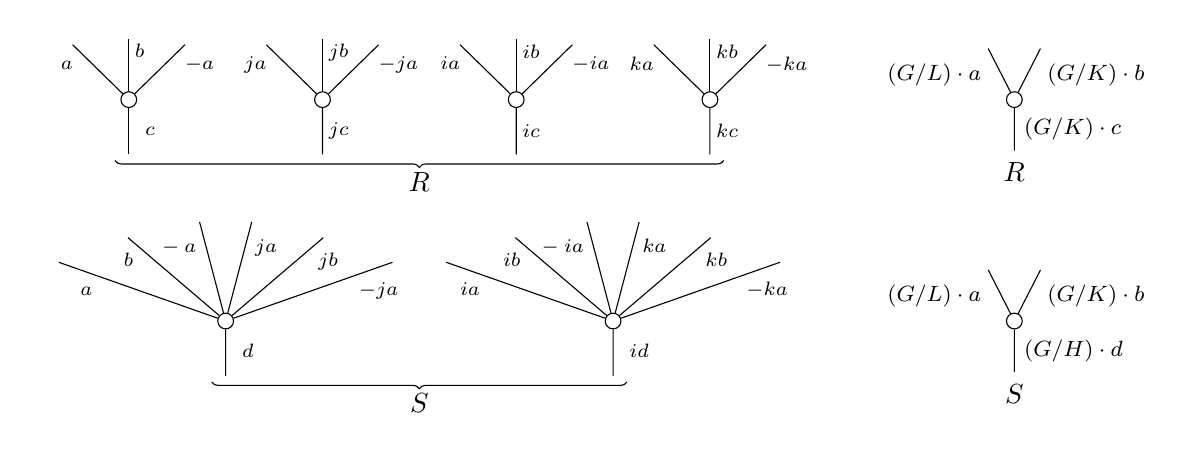
\begin{tikzpicture}[auto,grow=up, level distance = 2.2em,
	every node/.style={font=\scriptsize,inner sep = 2pt}]%
		\begin{scope}
		\tikzstyle{level 2}=[sibling distance=2.25em]%
			\node at (0,0){}%
				child{node [dummy] {}%
					child{node {}%
					edge from parent node [swap,very near end] {$-a\phantom{j}$}}%
					child[level distance = 2.4em]{node {}%
					edge from parent node [swap,near end] {$b\phantom{j}$}}%
					child{node {}%
					edge from parent node [very near end] {$\phantom{-j}a$}}%
				edge from parent node [swap] {$\phantom{j}c$}};%
			\node at (7em,0){}%
				child{node [dummy] {}%
					child{node {}%
					edge from parent node [swap,very near end] {$-j a$}}%
					child[level distance = 2.4em]{node {}%
					edge from parent node [swap,near end] {$j b$}}%
					child{node {}%
					edge from parent node [very near end] {$j a$}}%
				edge from parent node [swap] {$j c$}};%
			\node at (14em,0){}%
				child{node [dummy] {}%
					child{node {}%
					edge from parent node [swap,very near end] {$-i a$}}%
					child[level distance = 2.4em]{node {}%
					edge from parent node [swap,near end] {$i b$}}%
					child{node {}%
					edge from parent node [very near end] {$i a$}}%
				edge from parent node [swap] {$i c$}};%
			\node at (21em,0){}%
				child{node [dummy] {}%
					child{node {}%
					edge from parent node [swap,very near end] {$-k a$}}%
					child[level distance = 2.4em]{node {}%
					edge from parent node [swap,near end] {$k b$}}%
					child{node {}%
					edge from parent node [very near end] {$k a$}}%
				edge from parent node [swap] {$k c$}};%
		\end{scope}
		\begin{scope}[every node/.style={font=\footnotesize}]%
		\tikzstyle{level 2}=[sibling distance=2.25em]
			\node at (32em,0){}%
				child{node [dummy] {}%
					child{node {}%
					edge from parent node [swap,very near end] {$(G/K) \cdot b$}}%
					child{node {}%
					edge from parent node [very near end] {$(G/L) \cdot a$}}%
				edge from parent node [right] {$(G/K) \cdot c$}};%
		\end{scope}%
		\draw[decorate,decoration={brace,amplitude=2.5pt}] (21.5em,0) -- (-0.5em,0) node[midway,inner sep=4pt,font=\normalsize]{$R$}; %
		\node at (32em,-0.15) [font=\normalsize] {$R$};
%------- Second line ------
	\begin{scope}[yshift = -8em]
		\begin{scope}
		\tikzstyle{level 2}=[sibling distance=3em]%
			\node at (3.5em,0){}%
				child{node [dummy] {}%
					child[sibling distance=2.5em,level distance=2.2em]{node {}%
					edge from parent node [swap, near end] {$-ja\phantom{j}$}}%
					child[sibling distance=2.5em,level distance=3.2em]{node {}%
					edge from parent node [very near end,swap] {$j b\phantom{j}$}}%
					child[sibling distance=2em,level distance=3.8em]{node {}%
					edge from parent node [swap,very near end] {$j a$}}%
					child[sibling distance=2em,level distance=3.8em]{node {}%
					edge from parent node [very near end] {$\phantom{j}-a$}}%
					child[sibling distance=2.5em,level distance=3.2em]{node {}%
					edge from parent node [very near end] {$\phantom{j}b$}}%
					child[sibling distance=2.5em,level distance=2.2em]{node {}%
					edge from parent node [near end] {$\phantom{-j}a$}}%
				edge from parent node [swap] {$\phantom{j}d$}};%
			\node at (17.5em,0){}%
				child{node [dummy] {}%
					child[sibling distance=2.5em,level distance=2.2em]{node {}%
					edge from parent node [swap, near end] {$-ka\phantom{j}$}}%
					child[sibling distance=2.5em,level distance=3.2em]{node {}%
					edge from parent node [very near end,swap] {$k b\phantom{j}$}}%
					child[sibling distance=2em,level distance=3.8em]{node {}%
					edge from parent node [swap,very near end] {$k a$}}%
					child[sibling distance=2em,level distance=3.8em]{node {}%
					edge from parent node [very near end] {$\phantom{j}-ia$}}%
					child[sibling distance=2.5em,level distance=3.2em]{node {}%
					edge from parent node [very near end] {$\phantom{j}i b$}}%
					child[sibling distance=2.5em,level distance=2.2em]{node {}%
					edge from parent node [near end] {$\phantom{-j}i a$}}%
				edge from parent node [swap] {$\phantom{j}i d$}};%	
		\end{scope}
		\begin{scope}[every node/.style={font=\footnotesize}]%
		\tikzstyle{level 2}=[sibling distance=2.25em]%
			\node at (32em,0){}%
				child{node [dummy] {}%
					child{node {}%
					edge from parent node [swap,very near end] {$(G/K) \cdot b$}}%
					child{node {}%
					edge from parent node [very near end] {$(G/L) \cdot a$}}%
				edge from parent node [right] {$(G/H) \cdot d$}};%
		\end{scope}%
		\draw[decorate,decoration={brace,amplitude=2.5pt}] (18em,0) -- (3em,0) node[midway,inner sep=4pt,font=\normalsize]{$S$}; %
		\node at (32em,-0.15) [font=\normalsize] {$S$};
	\end{scope}
	\end{tikzpicture}%
\end{equation}%
These examples illustrate our motivation for the term 
``orbital face'': the tree diagrams in the orbital representations of $R,S$ look like faces of the tree in the orbital representation of $T$.

Adapting the notation for (non-equivariant) inner faces, we write
$S = T-Gc = T-\{c,jc,ic,kc\}$ and analogously throughout the paper.
We will need no analogous notation for orbital outer faces.
\end{example}


\begin{notation}\label{TREEDIFNOT NOT}
	In the remainder of the paper we sometimes need to consider (non-equivariant) and orbital faces simultaneously.
	As such, we reserve the letters $U,V,W$ for trees in $\Omega$
	and the letters $R,S,T$ for $G$-trees in $\Omega_G$.
\end{notation}


\begin{remark}\label{INNOUTORB REM}
	It follows from Proposition \ref{UNIQUEFACT PROP} that any orbital face $S \hookrightarrow T$ has a factorization
	$S \hookrightarrow R \hookrightarrow T$, unique up to isomorphism, as an orbital inner face followed by an orbital outer face.	
\end{remark}


\begin{proposition}\label{MINGFACT PROP}
	Let $T \in \Omega_G$.
	Any (non-equivariant) planar face $U \hookrightarrow T$ has a minimal factorization
	$U \hookrightarrow GU \hookrightarrow T$
	through a planar orbital face $GU$.
\end{proposition}

\begin{proof}
Assume first that $U=\bar{U}^T$ is outer and write $H\leq G$ for
the isotropy of its root $r_U$.
By Lemma \ref{CUPCAP LEM} there exists a smallest outer face 
containing all $\{h U \hookrightarrow T\}_{h \in H}$,
which we denote by $HU$.
Moreover, $HU$ inherits the $H$-action from $T$ 
(by either its construction or its characterization).
Moreover, the natural map
$G \cdot_H HU \to T$
is then injective on edges
(for a map of forests $F \to F'$
the images of the tree components of $F$ are pairwise $\leq_d$-incomparable iff so are the images of the roots)
and we thus let $GU$ be $G \cdot_H HU$
with the planar structure induced from $T$.
Both the factorization $U \to GU \to T$ and its minimality are immediate from the description of $HU$.

	Before tackling the general case, we collect some key observations.
	Firstly, if $U$ is outer then so is the (non-equivariant) face $HU$ and the orbital face $GU$.
	Secondly, the root tuple of 
	$GU$ is $G\cdot_H r_U$.
	Lastly, we need to characterize the leaf tuple of $GU$. We call a leaf $l$ of $U$ \textit{orbital} if 
all the edges in $Hl \cap E(U)$ are leaves of $U$, 
	and claim that the leaves of $GU$ are the tuple $\underline{l}$ formed by the $G$-orbits of the orbital leaves of $U$. 
	Indeed, a leaf $l$ of $U$ is also a leaf of $HU$ iff 
	$\forall_{h \in H}$ ($l \in E(hU)$ implies that $l$ is a leaf of $hU$) iff
	$\forall_{h \in H}$ ($h^{-1} l \in E(U)$ implies that $l$ is a leaf of $U$).
	
	In the general case, we define $GU$ as the orbital inner face of $G \bar{U}$ that removes all edge orbits not represented in $U$ 	(that all such edge orbits are inner follows from the description of the roots and leaves of $G\bar{U}$ in the previous paragraph). 
	It is now clear that $U \to G\bar{U} \to T$ is the minimal factorization with $G\bar{U}$ an \textit{outer} orbital face,
	and thus the factorization
	$U \to GU \to T$ exists and is minimal
	since inner faces are full (Remark \ref{INNFULL REM})
	together with the inner-outer factorization of
	orbital faces (Remark \ref{INNOUTORB REM}).
\end{proof}


\begin{example}
Much of the complexity in the previous proof is needed to handle  the scenario of non outer faces $U \hookrightarrow T$
of $G$-trees $T$ which have stumps,
which is easily the subtlest case, as illustrated by the following
example (where $G = \mathbb{Z}_{/2}=\{\pm1\}$).
\[%
	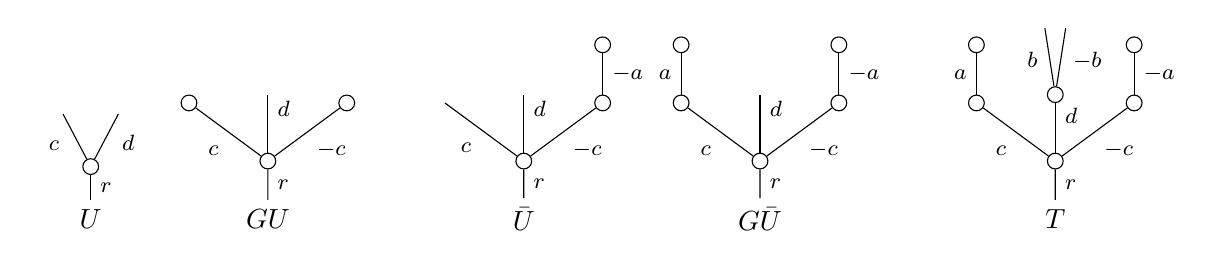
\begin{tikzpicture}[auto,grow=up, every node/.style = {font=\footnotesize}]%
	\begin{scope}[level distance = 1.9em]
	\tikzstyle{level 2}=[sibling distance=2em]%
	\tikzstyle{level 3}=[sibling distance=0.75em]%
		\node at (0,0) [font=\normalsize]{$U$}%
			child{node [dummy] {}%
				child{
				edge from parent node [swap, near end] {$d$}}%
				child{
				edge from parent node [near end] {$\phantom{d}c$}}%
			edge from parent node [swap] {$r$}};%
	\end{scope}
	\begin{scope}[level distance = 2.1em]
	\tikzstyle{level 2}=[sibling distance=2.85em]%
	\tikzstyle{level 3}=[sibling distance=0.75em]%
		\node at (2.25,0) [font=\normalsize]{$GU$}%
			child{node [dummy] {}%
				child{node [dummy] {}%
				edge from parent node [swap] {$-c$}}%
				child[level distance = 2.4em]{
				edge from parent node [near end,swap] {$d$}}%
				child{node [dummy] {}%
				edge from parent node {$\phantom{-}c$}}%
			edge from parent node [swap] {$r$}};%
		\node at (5.5,0) [font=\normalsize]{$\bar{U}$}%
			child{node [dummy] {}%
				child{node [dummy] {}%
					child{node [dummy] {}
					edge from parent node [swap] {$-a$}}%
				edge from parent node [swap] {$-c$}}%
				child[level distance = 2.4em]{
				edge from parent node [near end,swap] {$d$}}%
				child{
				edge from parent node {$\phantom{-}c$}}%
			edge from parent node [swap] {$r$}};%
		\node at (8.5,0) [font=\normalsize]{$G\bar{U}$}%
			child{node [dummy] {}%
				child{node [dummy] {}%
					child{node [dummy] {}
					edge from parent node [swap] {$-a$}}%
				edge from parent node [swap] {$-c$}}%
				child[level distance = 2.4em]{
				edge from parent node [near end,swap] {$d$}}%
				child{node [dummy] {}%
					child{node [dummy] {}
					edge from parent node {$\phantom{-}a$}}%
				edge from parent node {$\phantom{-}c$}}%
			edge from parent node [swap] {$r$}};%
		\node at (12.25,0) [font=\normalsize]{$T$}%
			child{node [dummy] {}%
				child{node [dummy] {}%
					child{node [dummy] {}
					edge from parent node [swap] {$-a$}}%
				edge from parent node [swap] {$-c$}}%
				child[level distance = 2.4em]{node [dummy] {}%
					child{
					edge from parent node [near end,swap]{$-b$}}%
					child{
					edge from parent node [near end]{$\phantom{-}b$}}%
				edge from parent node [near end,swap] {$d$}}%
				child{node [dummy] {}%
					child{node [dummy] {}
					edge from parent node {$\phantom{-}a$}}%
				edge from parent node {$\phantom{-}c$}}%
			edge from parent node [swap] {$r$}};%
	\end{scope}
	\end{tikzpicture}%
\]%

\end{example}

\begin{remark}
	It is clear from the proof of 
	Proposition \ref{MINGFACT PROP}
	that, if $U \in \mathsf{Face}(T)$ has isotropy $H$,
	the induced map 
	$G \cdot_H U \to T$ is a monomorphism iff
	$H$ is also the isotropy of the root $r_U$.
\end{remark}

\begin{remark}\label{GINNER REM}
	For any inner face $V-e$ of $V$ one has 
	that $G(V-e)$ is either $GV - Ge$ or $GV$.
	Indeed, the latter will happen iff $V-e$ contains either an inner edge of a leaf of the form $ge$.
\end{remark}

\begin{remark}
	Writing $\mathsf{Face}_o(T)$ for the poset of planar orbital faces, Proposition \ref{MINGFACT PROP} gives a $G$-equivariant functor (note that $G$ does not act on $\mathsf{Face}_o(T)$)
\[
	\mathsf{Face}(T) \xrightarrow{G(-)} \mathsf{Face}_o(T).
\]
Moreover, there is a natural inclusion
$\mathsf{Face}_o(T) \subseteq \mathsf{Face}(T)/G$ (sending an orbital face $S$ to the class of components $[S_{\**}]$)
whose left adjoint is the induced functor 
$\mathsf{Face}(T)/G \to \mathsf{Face}_o(T)$.
\end{remark}


\begin{remark}\label{ORB_FACE_REM}
	In fact, there is an isomorphism of posets
	\begin{equation}
	\mathsf{Face}_o(T) \xrightarrow{\simeq} \mathsf{Face}(T/G), \qquad S \mapsto S/G,
	\end{equation}
	where $T/G$ denotes the underlying tree in the orbital representation of $T$. 
	
	However, we caution that though this claim is  intuitive, care is needed when formalizing it.
	For example, the broad poset of $T/G$ is in general \textit{not} the quotient of the broad poset of $T$,
	as that may fail the simplicity axiom in 
	\cite[Def. 5.9]{Per17}.
	In fact, the assignment $T \mapsto T/G$ is \textit{not}
	a functor $\Omega_G \to \Omega$, as shown by
	the following (for $G = \mathbb{Z}_{/2} = \{\pm 1\}$),
	since no dashed arrow exists.
\begin{equation}
	\begin{tikzpicture}[auto,grow=up, level distance = 2.2em,
	every node/.style={font=\scriptsize,inner sep = 2pt}]%
		\tikzstyle{level 2}=[sibling distance=2.25em]%
		\begin{scope}
			\node at (0,0){}%
				child{node [dummy] {}%
					child{node {}%
					edge from parent node [swap,very near end] {$b\phantom{j}$}}%
					child{node {}%
					edge from parent node [very near end] {$\phantom{-j}a$}}%
				edge from parent node [swap] {$r\phantom{j}$}};%
			\node (T2) at (5em,0){}%
				child{node [dummy] {}%
					child{node {}%
					edge from parent node [swap,very near end] {$-a\phantom{j}$}}%
					child{node {}%
					edge from parent node [very near end] {$\phantom{j} -b$}}%
				edge from parent node [swap] {$-r$}};%
			\node (S) at (14em,0){}%
				child{node [dummy] {}%
					child{node {}%
					edge from parent node [swap,very near end] {$-a\phantom{j}$}}%
					child{node {}%
					edge from parent node [very near end] {$\phantom{j} a$}}%
				edge from parent node [swap] {$r$}};%
			\node at ($(S)+(0,-0.25)$) [font=\normalsize] {$S$};
		\draw[decorate,decoration={brace,amplitude=2.5pt}] (5.5em,0) -- (-0.5em,0) node[midway,inner sep=4pt,font=\normalsize]{$T$}; %
		\draw[->]
	($(T2) + (1,.75)$) -- ($(S)+(-1,.75)$) node [midway,above] {$b \mapsto -a$};
		\end{scope}%
%----Orbital picture-------
		\begin{scope}[xshift=25em]
			\node (TG) at (0,0){}%
				child{node [dummy] {}%
					child{node {}%
					edge from parent node {}}%
					child{node {}%
					edge from parent node {}}%
				edge from parent node {}};%
			\node at ($(TG) + (0,-0.25)$) [font=\normalsize] {$T/G$};
			\node (SG) at (9em,0){}%
				child{node [dummy] {}%
					child{node {}%
					edge from parent node {}}%
				edge from parent node {}};%
			\node at ($(SG) + (0,-0.25)$) [font=\normalsize] {$S/G$};
			\draw[->,dashed]
			($(TG) + (1,.75)$) -- ($(SG)+(-1,.75)$);
		\end{scope}
	\end{tikzpicture}%
\end{equation}%
We now outline the formal construction of $T/G$,
starting with some preliminary notation.

Given $\underline{e},\underline{f}$ tuples of edges of $T$, 
write $\underline{f} \leq \underline{e}$
if $\underline{e} = e_1 e_2 \cdots e_k$
and there is a tuple decomposition
$\underline{f} = 
\underline{f}_1 \underline{f}_2 \cdots
\underline{f}_k$
such that $\underline{f}_i \leq e_i$.
When the $e_i$ are $\leq_d$-incomparable,
\cite[Prop. 5.30]{Per17} says that such decomposition is unique, so that $\underline{e},\underline{f}$ consist of distinct edges and we can regard 
$\underline{e},\underline{f}$ as subsets $\underline{e},\underline{f} \subseteq E(T)$.
	
We now say that a relation
$\underline{f} \leq \underline{e}$	
is an \textit{orbital relation} if
$\underline{e} \subseteq E(T)$
is a orbital $G$-subset and $\underline{f} \subseteq E(T)$ is a $G$-subset. 
Reinterpreting the orbital relations of $T$ 
as broad relations on the set $E_{G}(T)$ of edge orbits,
one readily checks that this defines a 
dendroidally ordered set \cite[Def. 5.9]{Per17},
i.e. a tree, that we call $T/G$.
Note that one hence has a functor
$(-)/G \colon \Omega_G^+ \to \Omega$,
where $\Omega_G^+$ is the subcategory of orbital face maps,
and planarizations of the $T/G$ are chosen arbitrarily.

Lastly, we observe that, much as in the non-equivariant case,
the orbital outer faces of $T$ are indexed by orbital relations.
\end{remark}




\subsection{Equivariant dendroidal sets}

Recall \cite[\S 5.4]{Per17} that the category of 
\textit{$G$-equivariant dendroidal sets}
is the presheaf category 
$\mathsf{dSet}^G = \mathsf{Set}^{\Omega^{op} \times G}$.
Given $T \in \Omega_G$ with non-equivariant tree components $T_1,\cdots,T_k$,
we extend the usual notation for representable functors 
to obtain $\Omega[T] \in \mathsf{dSet}^G$ via
\[
	\Omega[T] = \Omega[T_1] \amalg \cdots \amalg \Omega[T_k]
\]
regarded as a $G$-object in $\mathsf{dSet}$.
One further defines \textit{boundaries} (in the union formula, 
the injection $\Omega[U] \to \Omega[T]$ is regarded as 
an inclusion; the equivalence between the colimit and union formulas follows from Proposition \ref{UNIQUEFACT PROP})
\[
	\partial \Omega[T] = 
	\mathop{\colim}_{U \in \mathsf{Face}(T),U \neq T_i}
	\Omega[U] =
	\bigcup_{U \in \mathsf{Face}(T),U \neq T_i}
	\Omega[U]
\]
and, for $\emptyset \neq E \subseteq E^{\mathsf{i}}(T)$ a
non-empty $G$-subset of inner edges 
(we abbreviate $E_i = E \cap E^{\mathsf{i}}(T_i)$), \textit{$G$-inner horns}
\[
	\Lambda^{E}[T] = 
	\mathop{\colim}_{U \in 
	\mathsf{Face}(T),
	(T_i - E_i) \not \hookrightarrow U}
	\Omega[U] =
	\bigcup_{U \in 
	\mathsf{Face}(T),
	(T_i - E_i) \not \hookrightarrow U}
	\Omega[U]
\]
which, informally, are the subcomplexes of $\Omega[T]$ that remove the inner faces $T_i-D$ for $D \subseteq E_i$.

Lastly, letting $\mathsf{Face}_{sc}(T)$ denote those outer faces of $T$ with no inner vertices (these are either single edges $t$ or generated by single vertices $t^{\uparrow} \leq t$), we define the 
\textit{Segal core of $T$}
\[
	Sc[T] 
= 
	\mathop{\colim}_{U \in 
	\mathsf{Face_{sc}}(T)}
	\Omega[U] 
=
	\bigcup_{U \in 
	\mathsf{Face}_{sc}(T)}
	\Omega[U].
\]

Note that if $T \simeq G \cdot_H T_{\**}$ for some $T_{\**} \in \Omega^H$ then 
\begin{equation}\label{T_DECOMP_EQ}
	\Omega[T] \simeq G \cdot_H \Omega[T_{\**}], 
\quad
	\partial \Omega[T] \simeq G \cdot_H \partial \Omega[T_{\**}], \quad
	\Lambda^{E}[T] \simeq G \cdot_H \Lambda^{E_{\**}}[T_{\**}],
\quad
	Sc[T] \simeq G \cdot_H Sc[T_{\**}].
\end{equation}
As a cautionary note, we point out that though representable functors $\Omega[T]$ are defined for $T \in \Omega_G$,
evaluations $X(U)$ of $X \in \mathsf{dSet}^G$
are defined only for $U \in \Omega$ (cf. Notation \ref{TREEDIFNOT NOT}).

\begin{remark}\label{FACEGACT REM}
	For $T \in \Omega_G$, a planar face $\varphi_U \colon U \to T$
	can also be regarded as a dendrex $\varphi_U \in \Omega[T](U)$.
	However, the $G$-isotropy $H$ of $U \in \mathsf{Face}(T)$ must not be confused with the $G$-isotropy of $\varphi_U$.
	Instead, $\Omega[T](U)$ has a larger $G \times \mathsf{Aut}(U)$-action,
	and the $G \times \mathsf{Aut}(U)$-isotropy of $\varphi_U$
	is a subgroup 
	$\Gamma \leq G \times \mathsf{Aut}(U)$
	which is the graph of a homomorphism
	$\phi\colon H \to \mathsf{Aut}(U)$.
	One readily checks that if $hU = U$ in $\mathsf{Face}(T)$ then
	$\phi(h)$ is the left isomorphism in \eqref{FACEGACT EQ},
	so that $U\in \Omega$ is equipped with a canonical $H$-action.
	We abuse notation by writing 
	$U \in \Omega^H \subseteq \Omega_H$ to denote this.  
\end{remark}

Recall that a class of maps is called \textit{saturated} if it is closed under pushouts, transfinite composition and retracts. 

The saturation of the boundary inclusions 
$\partial \Omega[T] \to \Omega[T]$
is the class of \textit{$G$-normal monormorphisms},
i.e. those monomorphisms $X \to Y$ in $\mathsf{dSet}^G$ such that
$Y(U) \setminus X(U)$ has an $\mathsf{Aut}(U)$-free action for all $U \in \Omega$. 
Moreover, since this condition is actually independent of the $G$-action, we will usually call these simply \textit{normal monomorphisms}.

The saturation of the $G$-inner horn inclusions 
$\Lambda^E[T] \to \Omega[T]$
is called the class of \textit{$G$-inner anodyne maps}, 
while those $X \in \mathsf{dSet}^G$
with the right lifting property against all $G$-inner horn inclusions are called \textit{$G$-$\infty$-operads}.

We can now recall \cite[Thm 2.1]{Per17}, which was the main result therein.

\begin{theorem}
	There is a model structure on $\mathsf{dSet^G}$
	such that the cofibrations are the normal monomorphisms and the fibrant objects are the $G$-$\infty$-operads.
\end{theorem}


\begin{remark}
The definition $G$-$\infty$-operads just given is a priori distinct from the original definition \cite[Def. 6.12]{Per17} which used only 
\textit{generating $G$-inner horn inclusion}, i.e. 
those inclusions $\Lambda^{Ge}[T] \to \Omega[T]$ with $E=Ge$ an inner edge orbit.
The present definition has the technical advantages of being naturally compatible with restricting the $G$-action and of allowing for a simpler proof of Lemma \ref{CHAREDGE LEM}, 
which is our main tool for showing that maps
are $G$-inner anodyne.
The equivalence between the two definitions follows from 
\cite[Prop. 6.17]{Per17},
although we also independently recover this 
from Lemma \ref{CHAREDGE LEM} in Corollary \ref{REGGENHORN COR}.
\end{remark}

In additional to the $G$-inner horns defined before, we now introduce a new kind of horn that, much like orbital faces,
is naturally suggested by the orbital representation of $G$-trees.
Given $E \subseteq E^{\mathsf{i}}(T)$ a $G$-equivariant set of inner edges, we define the associated 
\textit{orbital $G$-inner horn} by
\[
	\Lambda^{E}_o[T] = 
	\mathop{\colim}_{S \in 
	\mathsf{Face}_o(T),
	(T - E) \not \hookrightarrow S}
	\Omega[S] =
	\bigcup_{S \in 
	\mathsf{Face}_o(T),
	(T - E) \not \hookrightarrow S}
	\Omega[S]
\]
where we note that the equivalence between the colimit and union formulas now follows from Proposition \ref{MINGFACT PROP}.

\begin{remark}\label{ORB_HORN_REM}
We now extend the identification 
$\mathsf{Face}_o(T) \simeq \mathsf{Face}(T/G)$
in Remark \ref{ORB_FACE_REM}.

Say a subcomplex $A \subseteq \Omega[T]$ is \textit{orbital}
if it is the union of orbital faces $\Omega[S]$, $S\in \mathsf{Face}_o(T)$. 
Equivalently, by Proposition \ref{MINGFACT PROP} this means that for $U \in \mathsf{Face}(T)$
one has $\Omega[U] \subseteq A$ iff $\Omega[GU] \subseteq A$. There is then a natural bijection 
of posets (under inclusion)
\begin{equation}
	\set{
	\text{orbital subcomplexes $\bigcup_i\Omega[S_i]$ of $\Omega[T]$}}
		\leftrightarrow
	\set{\text{subcomplexes $\bigcup_i\Omega[S_i/G]$ of $\Omega[T/G]$}}.
\end{equation}
In particular, note that $\Lambda^{Ge}_o[T]$ corresponds to $\Lambda^{[e]}[T/G]$
and $Sc[T]$ corresponds to $Sc[T/G]$.
\end{remark}



\begin{example}
	Let $G = \mathbb{Z}_{/2} = \{\pm 1\}$,
      and consider the tree $T \in \Omega^G \subset \Omega_G$ below.
      \begin{equation}
            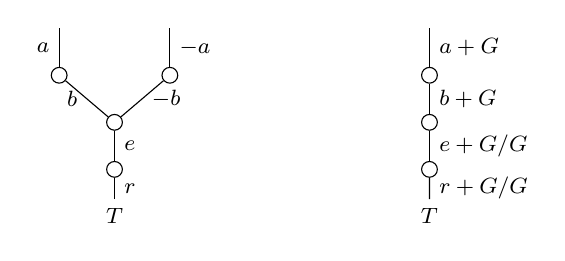
\begin{tikzpicture}[grow= up, level distance = 1.7em, every node/.style = {font=\footnotesize}]
                  \tikzstyle{level 2}=[sibling distance=4em]
                  \tikzstyle{level 3}=[sibling distance=4em]
                  \node{$T$}
                  child{node [dummy] {}
                    child{node [dummy] {}
                      child{node [dummy] {}
                        child{edge from parent node [right] {$-a$}}
                        edge from parent node [right] {$-b$}
                      }
                      child{node [dummy] {}
                        child{edge from parent node [left] {$a$}}
                        edge from parent node [left] {$b$}
                      }
                      edge from parent node [right] {$e$}
                    }
                    edge from parent node [right] {$r$}
                  };
                  \node at (4,0) {$T$}
                  child{node [dummy] {}
                    child{node [dummy] {}
                      child{node [dummy] {}
                        child{edge from parent node [right] {$a+G$}}
                        edge from parent node [right] {$b+G$}
                      }
                      edge from parent node [right] {$e+G/G$}
                    }
                    edge from parent node [right] {$r+G/G$}
                  };
            \end{tikzpicture}
      \end{equation}
      We compare the two horns discussed above by considering the subposet of $\mathsf{Face}(T)$
      displayed below in Figure \ref{HORN_EX_FIG}.
      The horn $\Lambda^{G e}[T]$ is only missing the faces $T$ and $T-r$,
      with maximal faces in $\Lambda^{G e}[T]$ given by the five faces in the top row;
      the maximal faces of the orbital horn $\Lambda^{G e}_o[T]$
      are those in the first two rows which are boxed.
      We have also included some of the subfaces of $S = \partial^{a}T$;
      those included in the orbital horn are (dashed) boxed.
      In particular, we note that $S$ and all of its maximal subfaces
      each have at least one face contained in the orbital horn. COME BACK
      \begin{figure}[ht]
            \label{HORN_EX_FIG}
            \begin{equation}
                  \newlength{\mywidth}
                  \setlength{\mywidth}{1.9em}%1.7
                  \newlength{\rowtwo}
                  \setlength{\rowtwo}{-2.6\mywidth}
                  \begin{tikzpicture}[grow= up, level distance = \mywidth, auto,
                        y=2\mywidth,
                        % dummy/.style    = {circle,draw,inner sep=0pt,minimum size=2mm}%
                        every node/.style = {font=\small, transform shape}
                        ,scale=.9
                        ]
                        \tikzstyle{level 2}=[sibling distance=4em]
                        \tikzstyle{level 3}=[sibling distance=4em]
                        \node (Paa) {}
                        child{node [dummy] {}
                          child{node [dummy] {}
                            child{
                              edge from parent node [swap] {$-b$}
                            }
                            child{node [dummy] {}
                              child{edge from parent node [] {$a$}}
                              edge from parent node [] {$b$}
                            }
                            edge from parent node [swap] {$e$}
                          }
                          edge from parent node [swap] {$r$}
                        };
                        \node (Pa) at (3.5,0) {$\partial^{a} T$}
                        child{node [dummy] {}
                          child{node [dummy] {}
                            child{node [dummy] {}
                              child{edge from parent node [swap] {$-a$}}
                              edge from parent node [swap] {$-b$}
                            }
                            child{
                              edge from parent node [] {$b$}
                            }
                            edge from parent node [swap] {$e$}
                          }
                          edge from parent node [swap] {$r$}
                        };
                        \node (Pr) at (7,0){$\partial^r$}
                        child{node [dummy] {}
                          child{node [dummy] {}
                            child{edge from parent node [swap] {$-a$}}
                            edge from parent node [swap] {$-b$}
                          }
                          child{node [dummy] {}
                            child{edge from parent node [] {$a$}}
                            edge from parent node [] {$b$}
                          }
                          edge from parent node [swap] {$e$}
                        };
                        \draw
                        (Pr)++(-1.25,-.2) rectangle ++(2.55,2);
                        \node (Tb) at (9.7,0){}
                        child{node [dummy] {}
                          child{node [dummy] {}
                            child{edge from parent node [swap] {$-a$}}
                            child{node [dummy] {}
                              child{edge from parent node [] {$a$}}
                              edge from parent node [] {$b$}
                            }
                            edge from parent node [swap] {$e$}
                          }
                          edge from parent node [swap] {$r$}
                        };
                        \node (Tbb) at (11.7,0) {}
                        child{node [dummy] {}
                          child{node [dummy] {}
                            child{node [dummy] {}
                              child{edge from parent node [swap] {$-a$}}
                              edge from parent node [swap] {$-b$}
                            }
                            child{
                              edge from parent node [] {$a$}
                            }
                            edge from parent node [swap] {$e$}
                          }
                          edge from parent node [swap] {$r$}
                        };
                        %%%%%%% --------- NEXT ROW -----------------------------
                        \node (PGa) at (0,-3.0) {$\partial^{G a}$} 
                        child{node [dummy] {}
                          child{node [dummy] {}
                            child{
                              edge from parent node [swap] {$-b$}
                            }
                            child{
                              edge from parent node [] {$b$}
                            }
                            edge from parent node [swap] {$e$}
                          }
                          edge from parent node [swap] {$r$}
                        };
                        \draw
                        (PGa)++(-1,-.2) rectangle ++(2,1.9);
                        % 
                        \node (TGb) at (10.7,-3.0) {$T - G b$}
                        child{node [dummy] {}
                          child{node [dummy] {}
                            child{
                              edge from parent node [swap] {$-a$}
                            }
                            child{
                              edge from parent node [] {$a$}
                            }
                            edge from parent node [swap] {$e$}
                          }
                          edge from parent node [swap] {$r$}
                        };
                        \draw
                        (TGb)++(-1,-.2) rectangle ++(2,1.9);
                        % -------- other orbital face of \partial{a}
                        \node (Par) at (7,-3.0) {$\partial^{a,r}$}
                        child{node [dummy] {}
                          child{node [dummy] {}
                            child{edge from parent node [swap] {$-a$}}
                            edge from parent node [swap] {$-b$}
                          }
                          child{edge from parent node [] {$b$}}
                          edge from parent node [swap] {$e$}
                        };
                        \draw[dashed]
                        (Par)++(-1,-.2) rectangle ++(2.25,1.9);
                        % ---------- other faces of \partial{a}
                        \node (Pae) at (2.3, -3) {$\partial^{a}-e$}
                        child{node [dummy] {}
                          child{node [dummy] {}
                            child{edge from parent node [swap] {$-a$}}
                            edge from parent node [swap] {$-b$}
                          }
                          child{edge from parent node [] {$b$}
                          }
                          edge from parent node [swap] {$r$}
                        };
                        \node (Pabb) at (4.7,-3) {$\partial^{a}-\set{-b}$}
                        child{node [dummy] {}
                          child{node [dummy] {}
                            child{edge from parent node [swap] {$-a$}}
                            child{edge from parent node [] {$b$}}
                            edge from parent node [swap] {$e$}
                          }
                          edge from parent node [swap] {$r$}
                        };
                        %%%% -------------------- next row --------------------
                        \node at (3.5, -5.5) {}
                        child{node [dummy] {}
                          child{edge from parent node [swap] {$-a$}}
                          child{edge from parent node [] {$b$}}
                          edge from parent node [swap] {$r$}
                        };
                        \node (Parb) at (7,-5.5) {}
                        child{node [dummy] {}
                          child{edge from parent node [swap] {$-a$}}
                          child{edge from parent node [] {$b$}}
                          edge from parent node [swap] {$e$}
                        };
                        \draw[dashed]
                        (Parb)++(-.9,-.1) rectangle ++(1.9,1.5);
                        % 
                        \node (PGae) at (0,-5.5) {}
                        child{node [dummy] {}
                          child{edge from parent node [swap] {$-b$}}
                          child{edge from parent node [] {$b$}}
                          edge from parent node [swap] {$r$}
                        };
                        \draw[dashed]
                        (PGae)++(-.9,-.1) rectangle ++(1.9,1.5);
                        %%%% -------------------- edges ----------
                        % ---------- conjugates ----------
                        \draw[<->]
                        (Pa)++(-.8,.5) -- (.8,.5) node [midway,above] {$+1$};
                        \draw[<->]
                        (Tbb)++(-.5,.5) -- ++(-1,0) node [midway,above] {$+1$};
                        % faces
                        \draw[->]
                        (Paa)++(0,-.3) -- ++(0,-.7);
                        \draw[->]
                        (Pr)++(0,-.3) -- ++(0,-.7);
                        \draw[->]
                        (Tb)++(0,-.3) -- ++(.5,-.7);
                        \draw[->]
                        (Tbb)++(0,-.3) -- ++(-.5,-.7);
                        % ---------- faces of Pa
                        \draw[->]
                        (Pa)++(-.2,-.2) -- ++(-2.5,-.8);
                        \draw[->]
                        (Pa)++(-.1,-.3) -- ++(-.7,-.7);
                        \draw[->]
                        (Pa)++(.1,-.3) -- ++(.7,-.7);
                        \draw[->]
                        (Pa)++(.2,-.2) -- ++(2.5,-.8);
                        % ---------- faces of Pab and Pae and Par and PGa
                        \draw[->]
                        (Pabb)++(-.2,-.4) -- ++(-.5,-.5);
                        \draw[->]
                        (Pabb)++(.2,-.4) -- ++(.5,-.5);
                        \draw[->]
                        (Pae)++(.2,-.4) -- ++(.5,-.5);
                        \draw[->]
                        (Pae)++(-.2,-.4) -- ++(-.5,-.5);
                        \draw[->]
                        (PGa)++(0,-.4) -- ++(0,-.5);
                        \draw[->]
                        (Par)++(0,-.4) -- ++(0,-.5);
                  \end{tikzpicture}
            \end{equation}
      \end{figure}
      % \begin{equation}
      %       \begin{tikzpicture}[grow= up, level distance = 1.7em, every node/.style = {font=\footnotesize}]
      %             \tikzstyle{level 2}=[sibling distance=4em]
      %             \tikzstyle{level 3}=[sibling distance=4em]
      %             \node{}
      %             child{node [dummy] {}
      %               child{node [dummy] {}
      %                 child{
      %                   edge from parent node [right] {$-b$}
      %                 }
      %                 child{node [dummy] {}
      %                   child{edge from parent node [left] {$a$}}
      %                   edge from parent node [left] {$b$}
      %                 }
      %                 edge from parent node [right] {$e$}
      %               }
      %               edge from parent node [right] {$r$}
      %             };
      %             \node at (3,0) {}
      %             child{node [dummy] {}
      %               child{node [dummy] {}
      %                 child{node [dummy] {}
      %                   child{edge from parent node [right] {$-a$}}
      %                   edge from parent node [right] {$-b$}
      %                 }
      %                 child{
      %                   edge from parent node [left] {$b$}
      %                 }
      %                 edge from parent node [right] {$e$}
      %               }
      %               edge from parent node [right] {$r$}
      %             };
      %             \node at (6,0){$\partial^r$}
      %             child{node [dummy] {}
      %               child{node [dummy] {}
      %                 child{edge from parent node [right] {$-a$}}
      %                 edge from parent node [right] {$-b$}
      %               }
      %               child{node [dummy] {}
      %                 child{edge from parent node [left] {$a$}}
      %                 edge from parent node [left] {$b$}
      %               }
      %               edge from parent node [right] {$e$}
      %             };
      %             \draw
      %             (4.5,-.3) rectangle ++(2.7,2.3);
      %             \node at (9,0){}
      %             child{node [dummy] {}
      %               child{node [dummy] {}
      %                 child{edge from parent node [right] {$-a$}}
      %                 child{node [dummy] {}
      %                   child{edge from parent node [left] {$a$}}
      %                   edge from parent node [left] {$b$}
      %                 }
      %                 edge from parent node [right] {$e$}
      %               }
      %               edge from parent node [right] {$r$}
      %             };
      %             \node at (12,0) {}
      %             child{node [dummy] {}
      %               child{node [dummy] {}
      %                 child{node [dummy] {}
      %                   child{edge from parent node [right] {$-a$}}
      %                   edge from parent node [right] {$-b$}
      %                 }
      %                 child{
      %                   edge from parent node [left] {$b$}
      %                 }
      %                 edge from parent node [right] {$e$}
      %               }
      %               edge from parent node [right] {$r$}
      %             };
      %             %%%%%%% --------- NEXT ROW -----------------------------
      %             \node at (0,-2) {$\partial^{G a}$}
      %             child{node [dummy] {}
      %               child{node [dummy] {}
      %                 child{
      %                   edge from parent node [right] {$-b$}
      %                 }
      %                 child{
      %                   edge from parent node [left] {$b$}
      %                 }
      %                 edge from parent node [right] {$e$}
      %               }
      %               edge from parent node [right] {$r$}
      %             };
      %             \node at (12,-2) {$T - G b$}
      %             child{node [dummy] {}
      %               child{node [dummy] {}
      %                 child{
      %                   edge from parent node [right] {$-a$}
      %                 }
      %                 child{
      %                   edge from parent node [left] {$a$}
      %                 }
      %                 edge from parent node [right] {$e$}
      %               }
      %               edge from parent node [right] {$r$}
      %             };
      %             \node at (6,-2) {$\partial^{a,r}$}
      %             child{node [dummy] {}
      %               child{node [dummy] {}
      %                 child{edge from parent node [right] {$-a$}}
      %                 edge from parent node [right] {$-b$}
      %               }
      %               child{edge from parent node [left] {$b$}}
      %               edge from parent node [right] {$e$}
      %             };
      %       \end{tikzpicture}
      % \end{equation}
\end{example}





\section{Equivariant inner anodyne maps}


Much as in \cite[\S 2]{CM13a}, 
it is essential for us to show that the inclusions $Sc[T] \to \Omega[T]$, $T\in \Omega_G$ are $G$-inner anodyne.
In addition, some parts of the equivariant dendroidal story are 
naturally described in terms of 
orbital $G$-inner horns $\Lambda^E_o[T]$ 
(rather than $G$-inner horns $\Lambda^E[T]$),
and one must hence also show that the inclusions
$\Lambda^E_o[T] \to \Omega[T]$
are $G$-inner anodyne.

In practice, the proofs of such results are long and somewhat repetitive, as they share many technical arguments.
Indeed, the case of orbital horns requires using many of the arguments in the long proof of \cite[Thm 7.1]{Per17}).

As such, we split our analysis into two parts.
In \S \ref{CHAREDGE SEC} we prove Lemma \ref{CHAREDGE LEM} which  we call the \textit{characteristic edge lemma} and
which abstractly identifies sufficient conditions for a map to be $G$-inner anodyne
(see Remark \ref{RECOVER REM} for a comparison with previous results in the literature).
%As an illustration of its power, we briefly summarize how 
%Lemma \ref{CHAREDGE LEM} significantly simplifies the proof of \cite[Thm 7.1]{Per17}.
Then, in \S \ref{HYPERSAT SEC} we deduce that the desired maps
are $G$-inner anodyne by applying Lemma \ref{CHAREDGE LEM}.



\subsection{The characteristic edge lemma} \label{CHAREDGE SEC}

\begin{definition}\label{CHAREDGE DEF}
      Let $T \in \Omega_G$, $A \subseteq \Omega[T]$ a subdendroidal set, and $\{U_i\}_{i \in I} \subseteq \mathsf{Face}(T)$ a subset.

      Given a set $\Xi^i$ of inner edges of $U_i$ and a subface $V \hookrightarrow U_i$, denote $\Xi_V^i = \Xi^i \cap E^{\mathsf{i}}(V)$.

      Suppose further that the indexing set $I$ is a 
      finite $G$-poset. For each $i \in I$ denote
      \[
            A_{<i} = A \cup \bigcup_{j \colon j<i} \Omega[U_j]
      \]
      We say that $\{\Xi^i \subseteq E^{\mathsf{i}}(U_i)\}$ 
      is a \textit{characteristic inner edge collection of $\{U_i\}$ with respect to $A$} if:
      \begin{itemize}
      \item[(Ch0)] $A$, $\{U_i\}$ and $\{\Xi^i\}$ are all $G$-equivariant, i.e. $g A = A$, $g U_i = U_{gi}$, $g \Xi^i = \Xi^{gi}$ as appropriate; 
      \item[(Ch1)] for all $i$, any outer face $V = \bar{V}^{U_i}$
            of $U_i$ such that $\Xi_{V}^i = \emptyset$
            is contained in $A_{<i}$;
      \item[(Ch2)] for all $i$, any face
            $V \hookrightarrow U_i$ such that $(V-\Xi_V^i) \in A$
            is contained in $A_{<i}$;
      \item[(Ch3)] for all $j \not \geq i$, 
            all faces $V \hookrightarrow U_i$ such that 
            $(V-\Xi^i_V) \hookrightarrow U_j$
            are contained in $A_{<i}$.
      \end{itemize}
\end{definition}


\begin{remark}\label{XIIII REM}
If $g i \neq i$, then $i,g i$ are incomparable in $I$. Indeed, otherwise $i<gi<g^2i<g^3i<\cdots$ would violate antisymmetry.
Therefore, (Ch3) applies whenever $j=gi$ for $gi\neq i$.

In particular, we assume throughout that if
$gi \neq i$ then $U_{gi} \neq U_i$,
or else it would be $U_i \in A_{<i}$.
\end{remark}


\begin{remark}\label{SOMEMAIN REM}
In some of the main examples (see Propositions \ref{ORB_HORN_PROP} and \ref{REG_HORN_PROP}), there exists a $G$-equivariant set 
$\Xi$ of inner edges of $T$ such that $\Xi^i = \Xi \cap E^{\mathsf{i}}(U_i)$.

%In such cases (Ch3) guarantees that, for fixed $\Xi$ and $A$, the characteristic conditions are monotone on $\{U_i\}$, in the sense that if they hold for $\{U_i\}$ they also hold for all of its subsets. NO LONGER TRUE
	
We caution that, for fixed $A$ and $\{U_i\}$, our characteristic conditions are \textit{not} monotone on such $\Xi$ since increasing $\Xi$ makes (Ch1) more permissive while making (Ch2),(Ch3) more restrictive.
\end{remark}


\begin{lemma}\label{CHAREDGE LEM}
If $\{\Xi^i\}_{i \in I}$ is a characteristic inner edge collection of $\{U_i\}_{i\in I}$ with respect to $A$, then the map
	\begin{equation}\label{CHARLEM EQ}
		A \to A \cup \bigcup_{i \in I} \Omega[U_i]
	\end{equation}
is $G$-inner anodyne. In fact, it is cellular on $G$-inner horn inclusions $\Lambda^E[S] \to \Omega[S]$, $S \in \Omega_G$.
\end{lemma}


\begin{proof}
We start with the case of $I \simeq G/H$ transitive so that, abbreviating $U = U_{[e]}$, $\{U_i\}$ is the set of conjugates $gU$. 
Note that $H$ is also the isotropy of $U$ in $\mathsf{Face}(T)$.
We likewise abbreviate $\Xi = \Xi^{[e]}$ and
$\Xi_V = \Xi_V^{[e]}$ for $V \hookrightarrow U$.
Moreover, in this case one has $A_{<[g]}=A$ in (Ch1),(Ch2),(Ch3).

We write $\mathsf{Face}_{\Xi}^{lex}(U)$
for the $H$-poset of planar faces $V \hookrightarrow U$
such that $\Xi_V \neq \emptyset$ and $\Xi_V = \Xi_{\bar{V}}$
ordered as follows: 
$V \leq V'$ if either
	\begin{inparaenum}
		\item[(i)] $\bar{V} \hookrightarrow \bar{V}'$ and 
		$\bar{V} \neq \bar{V}'$ or
		\item[(ii)] $\bar{V} = \bar{V}'$ and
		$V \hookrightarrow V'$
	\end{inparaenum}
(alternatively, this is the lexicographic order of pairs $(\bar{V},V))$.
We note that here and in the remainder of the proof all outer closures are implicitly taken in $U$ (rather than $T$), i.e. 
$\bar{V}=\bar{V}^U$.

For any $H$-equivariant convex subset $C$ of $\mathsf{Face}_{\Xi}^{lex}(U)$ we write
\[
A_C = 
A \cup \bigcup_{g\in G,V \in C} \Omega[gV].
\]
It now suffices to show that whenever
$C \subseteq C'$
the map 
$A_C \to A_{C'}$ is built cellularly from 
$G$-inner horn inclusions
(indeed, setting $C=\emptyset$ and 
$C'=\mathsf{Face}_{\Xi}^{lex}(U)$ recovers \eqref{CHARLEM EQ}
when $I \simeq G/H$).

Without loss of generality we can assume that $C'$ is obtained from $C$ by adding the $H$-orbit of a single $W \hookrightarrow U$. Further, we may assume $W \not \in A_C$ or else $A_C=A_{C'}$.
Letting $K \leq H$ denote the isotropy of 
$W$ in $\mathsf{Face}_{\Xi}^{lex}(U)$ and regarding $W \in \Omega^{K}\subseteq \Omega_{K}$, we claim there is a pushout diagram
\begin{equation}\label{FIRPUSH EQ}
\begin{tikzcd}
	G \cdot_{K} \Lambda^{\Xi_{W}}[W] \ar{d} \ar{r}&
	A_C \ar{d}
\\
	G \cdot_{K} \Omega[W] \ar{r}&
	A_{C'}
\end{tikzcd}
\end{equation}
where we note that inner edge set $\Xi_{W}$ is $K$-equivariant
since $\Xi_W = \Xi \cap E^{\mathsf{i}}(W)$ and $\Xi$ is $H$-equivariant by (Ch0).
The desired pushout will follow once we establish the following claims:
\begin{enumerate}
\item[(a)] all proper outer faces $V$ of $W$ are in $A_C$;
\item[(b)] an inner face $W - D$ of $W$ is in $A_C$ iff 
$D \not \subseteq \Xi_{W}$;
\item[(c)] 
the $G$-isotropy (i.e. the isotropy in $\mathsf{Face}(T)$)
of faces 
$W - D$, $D \subseteq \Xi_{W}$ is contained in $K$.
%the $G$-isotropy of inner faces 
%(i.e. their isotropy in $\mathsf{Face}(T)$)
%is contained in $G_W$.
\end{enumerate}

To check (a), writing $\bar{V}$ for the corresponding outer face of $U$, one has
	\[
	\Xi_V = \Xi \cap E^{\mathsf{i}} (V) 
	= \Xi \cap E^{\mathsf{i}}(W) \cap E^{\mathsf{i}}(\bar{V})
	= \Xi \cap E^{\mathsf{i}}(\bar{W}) \cap E^{\mathsf{i}}(\bar{V})
	= \Xi \cap E^{\mathsf{i}}(\bar{V})
	= \Xi_{\bar{V}}
	\]
where the second step follows from Lemma \ref{INNINT LEM}
(applied to $V \hookrightarrow W \hookrightarrow U$, 
$V \hookrightarrow \bar{V} \hookrightarrow U$)
and the third since by definition of
$\mathsf{Face}_{\Xi}^{lex}(U)$ it is $\Xi_{W} = \Xi_{\bar{W}}$.
Thus either $\Xi_V= \Xi_{\bar{V}} = \emptyset$ so that $\bar{V}\in A$ by (Ch1),
or $\Xi_V = \Xi_{\bar{V}} \neq \emptyset$
so that $V \in \mathsf{Face}_{\Xi}^{lex}(U)$ with $V<W$, and thus $V\in C$. In either case one has $V \in A_C$.

We now check the ``if'' direction of (b).
If $D \not \subseteq \Xi_{W}$
then $W' = W - (D \setminus \Xi_{W})$
is in $\mathsf{Face}_{\Xi}^{lex}(U)$
(since $\bar{W}' = \bar{W}$ and $\Xi_{W'} = \Xi_{W}$)
and $W'<W$, and thus $W' \in A_C$.

For the ``only if'' direction of (b), 
note first that it suffices to consider $D = \Xi_W$.
The assumption $W \not \in A_C$ together with (Ch2) imply that
$W'=W-\Xi_{W}$ is not in $A$, and thus it remains to show that 
$W'$ is not a face of any $gV$ with $g\in G$, $V \in C$.
Suppose otherwise, i.e. $W' \hookrightarrow gV$.
If it were $g \not \in H$, 
then it would be $W' \hookrightarrow gV \hookrightarrow g U \neq U$, and (Ch3) would imply $W\in A$. Thus we need only consider $g\in H$, and since $C$ is $H$-equivariant, we can set $g=e$.
It now suffices to show that if $W' \hookrightarrow V$
then it must be $W \leq V$ in $\mathsf{Face}_{\Xi}^{lex}(U)$,
since by convexity of $C$ this would contradict $W \not \in C$.
Since $W' \hookrightarrow V$ implies 
$\bar{W} = \bar{W}' \hookrightarrow \bar{V}$,
the condition $W \leq V$ is automatic from the definition of $\leq$ unless $\bar{W} = \bar{V}$.
In this latter case, by definition of 
$\mathsf{Face}_{\Xi}^{lex}(U)$ the face $V$ must contain as inner edges all edges in 
$\Xi_V=\Xi_{\bar{V}} = \Xi_{\bar{W}} = \Xi_{W}$,
so that not only $W - \Xi_{W} = W' \hookrightarrow V$ but also $W \hookrightarrow V$. But then it is $W \leq V$ in either case, establishing the desired contradiction. 

%\todo[inline]{What precisely is being contradicted is not clear on the first read through. I might reword the above as follows:}
%{\color{blue}
%  For the ``only if'' direction of (b), let $W' = W - \Xi_W$.
%  (Ch2) and the fact that $W \notin A_C$ together imply that $W' \notin A$,
%  and hence it remains to show that $W'$ is not a face of any $g V$ for $g \in G$, $V \in C$.
%  Suppose otherwise; say $W' \into g V$.
%  If $g \notin H$, then we would have $W' \into g V \into g U \neq U$,
%  and (Ch3) would imply $W \in A$.
%  Thus we need only consider $g \in H$, and since $C$ is $H$-equivariant, we may assume $g = e$.
%  But now since $W' \into V$, we have $\bar W = \bar W ' \into \bar V$.
%  We claim this implies $W < V$, contradicting $W \notin A_C$.
%  Indeed, either $\bar W \into \bar V$ with $\bar W \neq \bar V$, or,
%  if $\bar W = \bar V$, the definition of $\mathsf{Face}^{lex}_{\Xi}(U)$ implies that $V$ must contain all of
%  $\Xi_V = \Xi_{\bar V} = \Xi_{\bar W} = \Xi_{W}$ as inner edges,
%  and thus not only $W - \Xi_W = W' \into V$, but also $W \into V$.
%}

We now show (c).
If $g(W-D)=W-D$ then $g(W - \Xi_W) \hookrightarrow U$,
and thus $W - \Xi_W \hookrightarrow g^{-1}U$,
so that by (Ch3) it must be $g \in H$ or else it would be $W \in A$.
Now suppose $h(W-D)=W-D$ with $h\in H$.
Since $\Xi$ is $H$-equivariant (by (Ch0)) and
$\Xi_{W-D} = \Xi_{W} \setminus D$ (due to $D \subseteq \Xi_{W}$) it follows that 
$h(W-\Xi_W)=W-\Xi_W$,
so that we may assume $D=\Xi_W$.
Now note that
$hW$, $h(W-\Xi_W)=W-\Xi_W$, $W$
are all faces of $U$ with a common outer closure $\bar{W}$.
Hence
$h\Xi_{W} = \Xi_{hW} \subseteq \Xi_{\bar{W}} = \Xi_{W}$, where the last step follows since
$W \in \mathsf{Face}_{\Xi}^{lex}(U)$, and by cardinality reasons it must in fact be $h \Xi_{W} = \Xi_{W}$. But then $hW,W$
have the same outer closure and the same inner edges, and thus 
$hW=W$, establishing (c).


Lastly, we address the case of general $I$.
For each $G$-equivariant convex subset $J$ of $I$, set
\[
	A_J = 
	A \cup \bigcup_{j \in J} \Omega[U_j].
\]
As before, it suffices to check that for all convex subsets
$J \subseteq J'$
the map $A_J \to A_{J'}$ is built cellularly from $G$-inner horns,
and again we can assume that $J'$ is obtained from $J$ by adding a single $G$-orbit $Gj$ of $I$.
By the $I$ transitive case, it now suffices to check that
$\{\Xi^{gj}\}_{gj \in Gj}$ is also a characteristic inner edge collection of $\{U_{g j}\}_{g j \in Gj}$ with respect to $A_J$.
(Ch0) is clear, and since by $G$-equivariance and convexity it is $A_{<gj} \subseteq A_J$,
the new (Ch1),(Ch2),(Ch3)
conditions follow from the original conditions.
\end{proof}



\begin{remark}\label{CHAREDGE2 REM}
The requirement $A \subseteq \Omega[T]$ in Definition \ref{CHAREDGE DEF} can be relaxed.
Given an inclusion $A \subseteq B$,
a set of non-degenerate dendrices
$\{b_i \in B(U_i)\}_{i \in I}$
and a collection of edges
$\{\Xi^i \subset E^{\mathsf{i}}(U_i)\}_{i \in I}$, 
suppose that $I$ is a finite $G$-poset and that:
\begin{itemize}
	\item[(Ch0.1)] the maps $b_i \colon \Omega[U_i] \to B$ are monomorphisms;
	\item[(Ch0.2)] $A$, $\{U_i\}$ ,$\{b_i\}$ and $\{\Xi^i\}$
	are all $G$-equivariant in the sense that:
	\begin{inparaenum}
		\item[(i)] $gA = A$;
		\item[(ii)] there are associative and unital isomorphisms
		$U_i \xrightarrow{g} U_{g_i}$;
		\item[(iii)] the composites
		$\Omega[U_i] \xrightarrow{b_i} Y \xrightarrow{g} Y$
		and
		$\Omega[U_i]  \xrightarrow{g} \Omega[U_{gi}] \xrightarrow{b_{gi}} Y$ coincide;
		\item[(iv)] $g \Xi^i=\Xi^{gi}$.
	\end{inparaenum}
%	\item[(Ch0*3)] for each face $V \hookrightarrow U_i$ and $g \in G$
%	then $g y_i(V) = y_i(V)$ implies 
%	$g y_i(\bar{V}) = y_i(\bar{V})$.
\end{itemize}
Under (Ch0.1),
the $\Omega[U_i]$ are identified with subcomplexes of $B$,
and non-degenerate dendrices $b \in b_i(\Omega[U_i])(V)$
are identified with faces $V \hookrightarrow U_i$.

The original conditions (Ch1),(Ch2),(Ch3) can then be reinterpreted by, 
for each $V \hookrightarrow U_i$, 
regarding expressions such as $V \in A$, $(V-\Xi^i_V)\in U_j$
as $b_i(V) \in A$, $b_i(V-\Xi^i_V) \in b_j(\Omega[U_j])$.

The proof of Lemma \ref{CHAREDGE DEF} now carries through to show that 
\begin{equation}
	A \to A \cup \bigcup_{i \in I} b_i(\Omega[U_i])
\end{equation}
is $G$-inner anodyne (again built cellularly from $G$-inner horn inclusions).
%hence we note only the main differences.
%When writing the analogue of (\ref{FIRPUSH EQ}), 
%$K$ must be defined by noting that, cf. Remark \ref{FACEGACT REM},
%the $G \times \mathsf{Aut}(W)$-isotropy of 
%$y(W) \in y(\Omega[U])$
%is the graph of some partial homomorphism
%$G \geq K \xrightarrow{\phi} \mathsf{Aut}(W)$.
%Hence, when stating and proving the analogue of (c) one must instead deal with
%$G \times \mathsf{Aut}(W)$ and $G \times \mathsf{Aut}(W-D)$-isotropies.
%However, as explained in Remark \ref{FACEGACT REM}, the role of the $\mathsf{Aut}(W)$ and $\mathsf{Aut}(W-D)$ coordinates is simply to implement the replanarization isomorphism in (\ref{FACEGACT EQ}). 
%Hence, since non-degenerate $y' \in y(\Omega[U])$ are identified with faces in $\Omega^+\downarrow U$, by borrowing the notation in 
%Remark \ref{PLFUNCTOR REM}, the analogue of (c) states that if
%$pl(g y (W-D)) = y(W-D)$ then $pl(g y (W)) = y(W)$ 
%(note that $y(W)=pl(y(W))$ by definition of $W$).
%But reinterpreting the argument in the proof of Lemma \ref{CHAREDGE DEF}
%shows that $pl(g^{-1} y (W)),y(W)$ are planar faces of $U$ with the same closure and the same edges, and hence indeed 
%$pl(g y (W))=y(W)$.
\end{remark}


%\begin{example}
%To see the need for condition (Ch0*3),
%let $Y =\Delta[2] \amalg_{d_1(\Delta[1])} \Delta[2]$,
%where $d_1 \colon \Delta[1] \to \Delta[2]$
%is the inner face,
%together with the obvious $\mathbb{Z}_{/2}$-action.
%Then for $A = \Lambda^1[2] \amalg_{\partial \Delta[1]} \Lambda^1[2]$ and
%$\{y_i\}$ (resp. $\Xi$) the $\mathbb{Z}_{/2}$-orbital set
%consisting of the two copies of $\Delta[2]$ (resp. two copies of 
%$1 \in \Delta[2]$), 
%conditions (Ch0*1),(Ch0*2),(Ch1),(Ch2),(Ch3) all hold while (Ch0*3) fails,
%and one easily sees that $A \to Y$ is not built cellularly from 
%$\mathbb{Z}_{/2}$-inner horns.
%\end{example}


\begin{remark} \label{RECOVER REM}
Lemma \ref{CHAREDGE LEM} readily recovers several arguments in the literature:
\begin{itemize}
\item[(i)] In \cite[\S 10]{Rez01} (also \cite[\S 6.2]{Rez10}), Rezk introduces the notion of \textit{covers}, which in our language are the subsets
$Sc[n] \subseteq A \subseteq \Delta[n]$
such that if $V$ is in $A$ then so is the closure $\bar{V}^{[n]}$
(in words, $A$ is generated by outer faces).
Similarly, in the proof of \cite[Prop. 2.4]{CM13a}
Cisinski and Moerdijk use subcomplexes $S_j$ that can be regarded as
\textit{dendroidal covers},
i.e. subcomplexes
$Sc[T] \subseteq A \subseteq \Omega[T]$
such that if $V$ is in $A$ then so is $\bar{V}^{T}$.
Lastly, the subcomplexes 
$\Omega[T] \cup_l \Omega[S] \subseteq \Omega[T \circ_l S]$
in the grafting result \cite[Lemma 5.2]{MW09} (and similarly for the equivariant analogue \cite[Prop. 6.19]{Per17}) are also dendroidal covers.

Lemma \ref{CHAREDGE LEM} implies
that any inclusion $A \to A'$ of $G$-equivariant (dendroidal) covers of $T\in \Omega_G$
is $G$-inner anodyne. 
Indeed, let $I=\mathsf{Face}_{A'}^{out}(T)$ be the $G$-poset of outer faces $V \hookrightarrow T$ contained in $A'$, ordered by inclusion, 
$\Xi = E^{\mathsf{i}}(T)$ and $U_V = V$.
(Ch0) is clear, (Ch1) follows since 
$Sc(T) \subseteq A$, (Ch2) follows since $A$ is a cover and
(Ch3) follows since the $U_i$ are closed.

Alternatively, one can also use $I=\mathsf{Face}_{A',o}^{out}(T)$
for the $G$-trivial set of orbital outer faces 
$GV \hookrightarrow T$,
together with an \textit{arbitrary} total order (see Remark \ref{TWOPROOF REM} for a similar example).

Lastly, note that in the special case 
$\{U_i\}=\{T\}$, $\Xi=E^{\mathsf{i}}(T)$,
(Ch1) says precisely $Sc[T] \subseteq A$.


\item[(ii)] In \cite[Lemma 9.7]{MW09}, Moerdijk and Weiss introduced a \textit{characteristic edge} condition that can be regarded as a special case of our characteristic edge collection condition as generalized in Remark \ref{CHAREDGE2 REM}, and which served as one of our main inspirations.

Therein, they work in the case of $B= \Omega[T] \otimes \Omega[S]$
a tensor product of (non-equivariant) representable dendroidal sets, in which case (Ch0.1) is easily verified (and (Ch0.2) is moot).
In our notation, they then require that $I \simeq \**$ (so that (Ch3) is also moot), 
the dendrex 
$b_{\**} \in \left(\Omega[T] \otimes \Omega[S]\right)(U_{\**})$ encodes a special type of subtree $U_{\**}$ of $\Omega[T] \otimes \Omega[S]$, which they call an \textit{initial segment},
and they further require that $\Xi^{\**} = \{\xi\}$ is a singleton, called the \textit{characteristic edge}.
Moreover, they then demand that $A$ should contain all outer faces of the subtree $U_{\**}$, from which (Ch1) follows, 
as well as the key characteristic condition 
\cite[Lemma 9.7]{MW09}(ii),
which coincides with (Ch2) in this specific setting.

Similarly, in \cite[Lemma 7.39]{Per17} the second author introduced a \textit{characteristic edge orbit} condition that generalizes that in \cite{MW09} to the equivariant context 
by letting $I \simeq G/H$
and the $\Xi^{[g]}=\Xi \cap E^{\mathsf{i}}(U_{[g]})$ be determined by a $G$-edge orbit $\Xi \simeq Gf$ (cf. Remark \ref{SOMEMAIN REM}).

However, both of the lemmas in \cite{MW09} and \cite{Per17}
have the drawback of needing to be used iteratively
(so that much effort therein is spent showing that this can be done) while Lemma \ref{CHAREDGE LEM} is designed so that a single use suffices for the natural applications.
Indeed, conditions (Ch1) and (Ch3), the first of which relaxes the requirement in \cite{MW09},\cite{Per17} that $A$ should contain all outer faces, essentially provide abstract conditions under which the original characteristic edge arguments of \cite{MW09},\cite{Per17} can be iterated.
%Further, we note that in \cite{MW09},\cite{Per17} it is essential to make a good choice for the well-ordering in (Ch3).
%
%We end by noting the importance of the $G$-equivariance of $\Xi$
%in (Ch0),(Ch0*2). In proving \cite[Prop. 7.44]{Per17} the second author chose the $\Xi$ to be sets of edges of the subtrees $y_i$, and thus not necessarily $G$-equivariant,
%leading to the need of extra ad hoc arguments in that proof when establishing the analogue of condition (c) in the proof of Lemma \ref{CHAREDGE LEM}.
\end{itemize}
\end{remark}


\begin{example}\label{THM71 EX}
	As indicated above, Lemma \ref{CHAREDGE LEM} can be used to
	reorganize and streamline the rather long proofs of \cite[Thms 7.1 and 7.2]{Per17}. We illustrate this in the hardest case, that of \cite[Thm. 7.1(i)]{Per17}, which states that if
	$S,T \in \Omega_G$ are open (i.e. have no stumps) and
	$G \xi$ is an inner edge orbit of $T$ the maps
\begin{equation}\label{THM71 EQ}
	\partial \Omega[S] \otimes \Omega[T]
		\coprod_{\partial \Omega[S] \otimes \Lambda^{G\xi}[T]}
	\Omega[S] \otimes \Lambda^{G\xi}[T]
\to
	 \Omega[S] \otimes \Omega[T]
\end{equation}
are $G$-inner anodyne.

% As detailed in \cite[\S 5.1]{Per17},
% and originally due to Weiss in \cite{Wei12},
% there is an algebraically flavoured model for $\Omega$
% as certain types of \textit{broad posets}.
Given $S,T \in \Omega_G$, it is possible \cite[\S 7.1]{Per17} to define a $G$-equivariant broad poset $S \otimes T$
so that 
$\left(\Omega[S] \otimes \Omega[T]\right)(V) = Hom(V,S \otimes T)$
where the Hom set is taken in broad posets.
Intuitively $S \otimes T$ is an object with edge set $E(S) \times E(T)$
and where each edge $(s,t) \in S \otimes T$
may, depending on whether $s \in S$, $t \in T$ are leaves or not,
admit two \textit{distinct} vertices: a $S$-vertex 
$(s,t)^{\uparrow S} = s^{\uparrow} \times t \leq (s,t)$
and a $T$-vertex
$(s,t)^{\uparrow T} = s \times t^{\uparrow} \leq (s,t)$.

To recover \cite[Thm. 7.1(i)]{Per17} from Lemma \ref{CHAREDGE LEM}, we first let $I = \mathsf{Max}(S \otimes T)$
be the $G$-poset of maximal subtrees $U \hookrightarrow S \otimes T$ 
(these are called \textit{percolation schemes} in \cite[\S 9]{MW09}), ordered lexicographically \cite[Def. 7.29]{Per17}.
As an example, let $\mathbb{Z}_{/2} = \{\pm 1\}$
and consider the $\mathbb{Z}_{/2}$-trees
\[%
	\begin{tikzpicture}[auto,grow=up, every node/.style = {font=\footnotesize}]%
	\begin{scope}[level distance = 2.1em]
	\tikzstyle{level 2}=[sibling distance=3em]%
	\tikzstyle{level 3}=[sibling distance=2.5em]%
		\node at (0,0) {$S$}%
			child{node [dummy,fill=black] {}%
				child{
				edge from parent node [near end,swap] {$-1$}}%
				child{
				edge from parent node [near end]{$\phantom{-}1$}}%
			edge from parent node [swap] {$0$}};%
		\node at (4,0) {$T$}%
			child{node [dummy] {}%
				child{node [dummy] {}
					child{
					edge from parent node[swap]{$-a\phantom{-}$}}
				edge from parent node [near end,swap] {$-\xi\phantom{-}$}}%
				child{node [dummy] {}
					child{
					edge from parent node{$\phantom{-}a$}}
				edge from parent node [near end]{$\phantom{-}\xi$}}%
			edge from parent node [swap] {$r$}};%
	\end{scope}
	\end{tikzpicture}%
\]%
We depict the $\mathbb{Z}_{/2}$-poset 
$\mathsf{Max}(S \otimes T)$
in Figure \ref{FIGURE} (note that $(s,t)$ is abbreviated as $t_s$).
In words, the maximal subtrees are built by starting with the
``double root'' $r_0$ and iteratively choosing between the available $S$ and $T$ vertices (along all upward paths) until the 
``double leaves'' are reached.
The generating relations $U \leq U'$ in 
$\mathsf{Max}(S \otimes T)$
occur whenever $U$ contains an outer face $V$ shaped as on the left below and, by ``replacing'' $V$ with $V'$ as on the right, one obtains $U'$.
\begin{equation}\label{GENLEXREL EQ}
	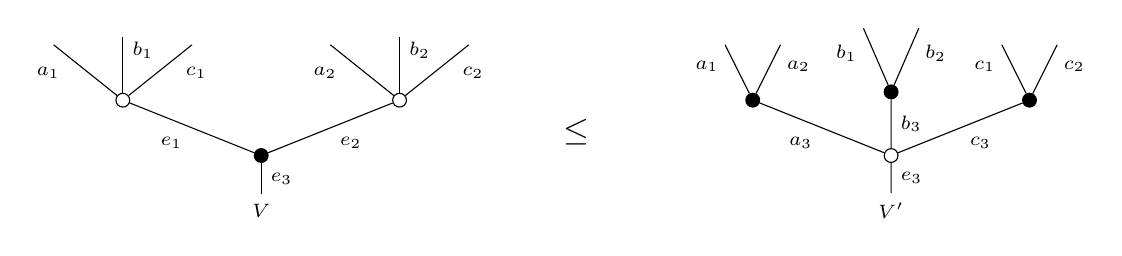
\begin{tikzpicture}[auto,grow=up, level distance = 2em,
	every node/.style={font=\scriptsize},
	dummy/.style = {circle,draw,inner sep=0pt,
	minimum size=1.75mm}]
	\begin{scope}
	\tikzstyle{level 2}=[sibling distance=10em]%
	\tikzstyle{level 3}=[sibling distance=2.5em]%
		\node at (0,0) {$V$}
			child{node [dummy,fill=black] {}
				child{node [dummy] {}
					child{
					edge from parent node [swap,near end] {$c_2$}}
					child[level distance = 2.3em]{
					edge from parent node [swap, near end] {$b_2$}}
					child{
					edge from parent node [near end] {$a_2$}}
				edge from parent node [swap] {$e_2$}}
				child{node [dummy] {}
					child{
					edge from parent node [swap,near end] {$c_1$}}
					child[level distance = 2.3em]{
					edge from parent node [swap, near end] {$b_1$}}
					child{
					edge from parent node [near end] {$a_1$}}				
				edge from parent node {$e_1$}}
			edge from parent node [swap] {$e_3$}};
	\end{scope}
	\begin{scope}
	\tikzstyle{level 2}=[sibling distance=5em]%
	\tikzstyle{level 3}=[sibling distance=2em]%
		\node at (8,0) {$V'$}
			child{node [dummy] {}
				child{node [dummy,fill=black] {}
					child{
					edge from parent node [swap,very near end] {$c_2$}}
					child{
					edge from parent node [very near end] {$c_1$}}
				edge from parent node [swap] {$c_3$}}
				child[level distance = 2.3em]{node [dummy,fill=black] {}
					child{
					edge from parent node [swap,very near end] {$b_2$}}
					child{
					edge from parent node [very near end] {$b_1$}}
				edge from parent node [swap] {$b_3$}}
				child{node [dummy,fill=black] {}
					child{
					edge from parent node [very near end,swap] {$a_2$}}
					child{
					edge from parent node [very near end] {$a_1$}}				
				edge from parent node {$a_3$}}
			edge from parent node [swap] {$e_3$}};
		\node at (4,1) [font=\large] {$\leq$};
	\end{scope}
	\end{tikzpicture}
\end{equation}
The claim that $\leq$ is indeed a partial order 
(at least if one of $S,T$ is open) is 
\cite[Prop. 7.31]{Per17}.
As an aside, we note that   
$V,V'$ above have a common inner face
$V-\{e_1,e_2\} = V'-\{a_3,b_3,c_3\}$,
which encodes an (universal!) example of a 
Boardman-Vogt relation (see \cite[\S 5.1]{MW07}).
\begin{figure}[ht]
\[%
	\begin{tikzpicture}[auto,grow=up, every node/.style = {font=\footnotesize}]%
	\begin{scope}[level distance = 1.9em]
	\tikzstyle{level 2}=[sibling distance=8em]%
	\tikzstyle{level 3}=[sibling distance=2.5em]%
	\tikzstyle{level 4}=[sibling distance=2em]%
		\node at (0,-0.5) {$\Xi^1=\{\xi_1,-\xi_1,\xi_{-1},-\xi_{-1}\}$};%
		\node at (0,0) {$U_1$}%
			child{node [dummy,fill=black] {}%
				child{node [dummy] {}%
					child{node [dummy] {}
						child{
						edge from parent node[swap]{$-a_{-1}$}}
					edge from parent node [near end,swap] {$-\xi_{-1}$}}%
					child{node [dummy] {}
						child{
						edge from parent node{$\phantom{-}a_{-1}$}}
					edge from parent node [near end]{$\phantom{-}\xi_{-1}$}}%
				edge from parent node [swap] {$r_{-1}$}}%
				child{node [dummy] {}%
					child{node [dummy] {}
						child{
						edge from parent node[swap]{$-a_1$}}
					edge from parent node [near end,swap] {$-\xi_1$}}%
					child{node [dummy] {}
						child{
						edge from parent node{$\phantom{-}a_1$}}
					edge from parent node [near end]{$\phantom{-}\xi_1$}}%
				edge from parent node {$r_{1}$}}%
			edge from parent node [swap] {$r_0$}};
		\node at (0,3.5) {$\Xi^2=\{\xi_1,\xi_{-1}-\xi_1,-\xi_{-1}\}$};%
		\node at (0,4) {$U_2$}%
			child{node [dummy] {}%
				child{node [dummy,fill=black] {}%
					child{node [dummy] {}
						child{
						edge from parent node[swap]{$-a_{-1}$}}
					edge from parent node [near end,swap] {$-\xi_{-1}$}}%
					child{node [dummy] {}
						child{
						edge from parent node{$-a_{1}$}}
					edge from parent node [near end]{$-\xi_{1}$}}%
				edge from parent node [swap] {$-\xi_0$}}%
				child{node [dummy,fill=black] {}%
					child{node [dummy] {}
						child{
						edge from parent node[swap]{$a_{-1}\phantom{-}$}}
					edge from parent node [near end,swap] {$\xi_{-1}\phantom{-}$}}%
					child{node [dummy] {}
						child{
						edge from parent node{$\phantom{-}a_1$}}
					edge from parent node [near end]{$\phantom{-}\xi_1$}}%
				edge from parent node {$\xi_0$}}%
			edge from parent node [swap] {$r_0$}};
		\node at (-4.75,6.5) {$\Xi^3=\{\xi_0,-\xi_1,-\xi_{-1}\}$};%
		\node at (-4.75,7) {$U_3$}%
			child{node [dummy] {}%
				child{node [dummy,fill=black] {}%
					child{node [dummy] {}
						child{
						edge from parent node[swap]{$-a_{-1}$}}
					edge from parent node [near end,swap] {$-\xi_{-1}$}}%
					child{node [dummy] {}
						child{
						edge from parent node{$-a_{1}$}}
					edge from parent node [near end]{$-\xi_{1}$}}%
				edge from parent node [swap] {$-\xi_0$}}%
				child{node [dummy] {}%
					child{node [dummy,fill=black] {}
						child{
						edge from parent node [swap,near end]{$a_{-1}\phantom{-}$}}
						child{
						edge from parent node [near end] {$\phantom{-}a_{1}$}}
					edge from parent node {$a_0$}}%
				edge from parent node {$\xi_0$}}%
			edge from parent node [swap] {$r_0$}};
		\node at (4.75,6.5) {$-\Xi^3=\{\xi_1,\xi_{-1},-\xi_0\}$};%
		\node at (4.75,7) {$-U_3$}%
			child{node [dummy] {}%
				child{node [dummy] {}%
					child{node [dummy,fill=black] {}
						child{
						edge from parent node [swap,near end]{$-a_{-1}$}}
						child{
						edge from parent node [near end] {$-a_{1}$}}
					edge from parent node [swap] {$-a_0$}}%
				edge from parent node [swap] {$-\xi_0$}}%
				child{node [dummy,fill=black] {}%
					child{node [dummy] {}
						child{
						edge from parent node[swap]{$a_{-1}\phantom{-}$}}
					edge from parent node [near end,swap] {$\xi_{-1}\phantom{-}$}}%
					child{node [dummy] {}
						child{
						edge from parent node{$\phantom{-}a_1$}}
					edge from parent node [near end]{$\phantom{-}\xi_1$}}%
				edge from parent node {$\xi_0$}}%
			edge from parent node [swap] {$r_0$}};
		\node at (0,8.5) {$\Xi^4=\{\xi_0,-\xi_0\}$};%
		\node at (0,9) {$U_4$}%
			child{node [dummy] {}%
				child{node [dummy] {}%
					child{node [dummy,fill=black] {}
						child{
						edge from parent node [swap,near end]{$-a_{-1}$}}
						child{
						edge from parent node [near end] {$-a_{1}$}}
					edge from parent node [swap] {$-a_0$}}%
				edge from parent node [swap] {$-\xi_0$}}%
				child{node [dummy] {}%
					child{node [dummy,fill=black] {}
						child{
						edge from parent node [swap,near end]{$a_{-1}\phantom{-}$}}
						child{
						edge from parent node [near end] {$\phantom{-}a_{1}$}}
					edge from parent node {$a_0$}}%
				edge from parent node {$\xi_0$}}%
			edge from parent node [swap] {$r_0$}};
	\end{scope}
	\end{tikzpicture}%
\]%
\caption{The $\mathbb{Z}_{/2}$-poset $\mathsf{Max}(S \otimes T)$ and characteristic edges $\Xi^i$}
\label{FIGURE}
\end{figure}

Returning to the task of proving that \eqref{THM71 EQ} is $G$-inner anodyne, we define $\Xi^U$, 
for each maximal subtree $U \hookrightarrow S \otimes T$,
to be the set of inner edges of $U$ of the form
$(g \xi)_s$ \textit{such that}
the vertex $(g \xi)_s^{\uparrow U} \leq (g \xi)_s$ in $U$
is a $T$-vertex (see Figure \ref{FIGURE}).
We now verify (Ch1),(Ch2),(Ch3).
We recall that, since $S,T$ are assumed open,
\cite[Lemma 7.19]{Per17} guarantees that,
for faces
$S' \hookrightarrow S$, $T' \hookrightarrow T$,
a factorization
$V \hookrightarrow S' \otimes T' \hookrightarrow S \otimes T$
exists iff the edges of $V$ are in $E(S') \times E(T')$.

For (Ch1), note first that there is an equivariant grafting decomposition
$T = T_{\not < G\xi} \amalg_{G \xi} T^{\leq G\xi}$, 
where $T_{\not < G\xi}$ contains the edges $t \in T$ such that
$\forall_{g \in G} t \not < g\xi$ (pictorially, this is a lower equivariant outer face of $T$) 
while $T^{\leq G\xi}$
contains the edges $t \in T$ such that
$\exists_{g \in G} t \leq g\xi$ (an upper equivariant outer face of $T$).
But one now readily checks that if
$V \hookrightarrow U$ is an \textit{outer} face such that
$\Xi^U_V = \emptyset$, then either 
$V \hookrightarrow S \otimes T_{\not < G\xi}$ or 
$V \hookrightarrow S \otimes T^{\leq G\xi}$, and thus $V \in A$.

For (Ch3), suppose $U_j \not \geq U_i$, 
$V \hookrightarrow U_i$ and
$(V - \Xi^{U_i}_V) \hookrightarrow U_j$.
Then it follows from \cite[Lemma 7.37]{Per17}
that there exists a generating relation $U_k < U_i$
such that $(V - \Xi^{U_i}_V) \hookrightarrow U_k$
(indeed, \cite[Lemma 7.37]{Per17} makes the slightly stronger claim that such a relation can be performed on the outer closure $\bar{V}^{U_i}$). But then, as one sees from \eqref{GENLEXREL EQ},
all edges $e \in U_i$ that are not in $U_k$ are topped by the $S$-vertex $e^{\uparrow S}\leq e$, and thus it is $e \not \in \Xi^{U_i}$. Therefore $V \hookrightarrow U_k$, as desired.

Lastly, for (Ch2), suppose $V \hookrightarrow U$ and 
$(V - \Xi^{U}_V) \in A$.
If it were 
$(V-\Xi^{U}_V) \hookrightarrow S \otimes \Lambda^{G \xi}[T]$, then it would also be 
$V \hookrightarrow S \otimes \Lambda^{G \xi}[T]$
since all edges of $\Xi^{U}_V$ have 
$T$-coordinate in $G\xi$.
Now consider the more interesting case
$(V - \Xi^{U}_V) \hookrightarrow S' \otimes T$
for some face $S' \hookrightarrow S$.
Then it will also be 
$V \hookrightarrow S' \otimes T$
unless there is at least one edge
$(g \xi)_s \in \Xi^{U}_V$ such that $s \not \in S'$.
But then since the outer closure $\bar{V}^U$ can have no leaf with $S$-coordinate $s$ (this would contradict $s \not \in S'$),
there exists some minimal outer face $U_{(g\xi)_s}^{<s}$ of $U$ with root $(g\xi_s)$ and such that its leaves have $S$-coordinate $<_d s$.
By minimality, one has that $U_{(g\xi)_s}^{<s} \hookrightarrow \bar{V}^U$ and that all inner edges of $U_{(g\xi)_s}^{<s}$ have
$S$-coordinate $s$.
Further, note that $U_{(g\xi)_s}^{<s}$
has at least one inner edge
(since by definition of $\Xi^U$ the vertex 
$(g \xi)_s^{\uparrow U} \leq (g \xi)_s$ is a $T$-vertex)
and that $V$ contains none of those inner edges (or else it would be $s \in S'$).
Thus by applying \cite[Lemma 7.34]{Per17}
to $U_{(g\xi)_s}^{<s}$ one obtains a maximal subtree $U' < U$
containing all edges of $U$ that are not inner edges of $U_{(g\xi)_s}^{<s}$.
But then $V \hookrightarrow U'$ and (Ch2) follows.
\end{example}

 
\begin{remark}
We briefly outline how to modify the previous example to prove 
\cite[Thm 7.1(ii)]{Per17}, in which case some notable subtleties arise.
The result again states that \eqref{THM71 EQ} is $G$-inner anodyne, but now with one of $S,T$ allowed to have stumps while the other is required to be linear.

One again sets $I=\mathsf{Max}(S\otimes T)$, where maximal trees are defined just as before, but some care is now needed.
To see why, note that if the black nodes $\bullet$ in \eqref{GENLEXREL EQ} are replaced with stumps then $V'$
is actually a subtree of $V$.

When $S$ has stumps and $T$ is linear this causes no issues and the proof above holds
(though we note that it can now be 
$\Xi^U=\emptyset$, in which case the argument for (Ch1) shows $U\in A$).

However, when $S$ is linear and $T$ has stumps the proof above breaks down (more precisely, the tree $U_{(g\xi)_s}^{<s}$ that appears when arguing (Ch2) may now fail to have inner edges). The solution is then to \textit{reverse} the poset structure on 
$\mathsf{Max}(S\otimes T)$
and to modify the $\Xi^U$ to be those inner edges $(g \xi)_s$ such that
$(g _xi)_s \in t_s^{\uparrow T}$ for some $t_s$
(pictorially, this says that these are the lowermost edges with $T$-coordinate in $G\xi$, whereas before they were the uppermost ones). The arguments for (Ch1),(Ch3) then hold.
For (Ch2), only the argument for the interesting case of
$V- \Xi_V^U \hookrightarrow S' \otimes T$, $s \not \in S'$
changes. In this case, there is then a maximal edge $t'_s$ such that $(g \xi)_s < t'_s$, where $s$ can not be the root of $S$ (or else it would be $s \in S'$). Pictorially, $t'_s$ looks like the edge $e_1 \in V$ in \eqref{GENLEXREL EQ} in the case where the $\bullet$ node is unary (since $S$ is assumed linear). But then since $V$ can not contain $t'_s$ there exists a maximal subtree $U' > U$ such that $V \hookrightarrow U'$,
and (Ch2) follows.

Lastly, we note that \cite[Thm. 7.2]{Per17} follows from a minor variant of the argument for \cite[Thm. 7.1(ii)]{Per17} when $S$ is linear.
\end{remark}



\subsection{Segal cores, horns and orbital horns}\label{HYPERSAT SEC}


\begin{proposition}\label{ORB_HORN_PROP}
	For $G$-subsets  
	$\emptyset \neq F \subseteq E \subseteq E^{\mathsf{i}}(T)$
	the inclusions
\begin{equation}\label{ORBHORNINC EQ}
	\Lambda_o^{E}[T] \to \Omega[T],\qquad
	\Lambda_o^{E}[T] \to \Lambda_o^{F}[T]
\end{equation}
	are $G$-inner anodyne.
\end{proposition}


\begin{proof}
We are free to assume that $T \in \Omega^G \subseteq \Omega_G$. Indeed, otherwise writing $T = G \cdot_H T_{\**}$, where $T_{\**} \in \Omega^H$ is a fixed component and 
$E_{\**}=E \cap E^{\mathsf{i}}(T_{\**})$, $F_{\**} = F \cap E^{\mathsf{i}}(T_{\**})$,
the maps in \eqref{ORBHORNINC EQ} are
$G \cdot_H 
\left( \Lambda_o^{E_{\**}}[T_{\**}] \to \Omega[T_{\**}]\right)$
and
$G \cdot_H 
\left( \Lambda_o^{E_{\**}}[T_{\**}] \to \Lambda_o^{F_{\**}}[T_{\**}]\right)$.

In the $\Lambda_o^{E}[T] \to \Omega[T]$ case we apply
Lemma \ref{CHAREDGE LEM} with $I = \{\**\}$ a singleton and
\[
	\Xi^{\**} = E, \qquad 
	U_{\**} = T,\qquad
	A=\Lambda_o^{E}[T].
\]
It remains to check the characteristic conditions in Definition \ref{CHAREDGE DEF}.
	(Ch0) and (Ch3) are clear.

Note that for $V\hookrightarrow T$ it is $V \not \in A$ iff 
$GV = T-E'$ for some $G$-subset
$E' \subseteq E$.

For (Ch1), the condition $\Xi_{V} = \emptyset$
says that none of the inner edges of $V$ are in $E$,
and thus that the orbital outer face $G V$ contains none of the edge orbits in $E$ as inner edge orbits. Since $E \neq \emptyset$, the orbital outer face $GV$ is not $T$ itself, 
and hence $A=\Lambda_o^{E}[T]$ contains $V$.

For (Ch2), note that if $V \not \in A$, i.e., 
$GV = T - E'$, then Remark \ref{GINNER REM} implies that
$G(V-\Xi_V) = T - E''$ for $E'\subseteq E'' \subseteq E$,
and thus also $(V-\Xi_V) \not \in A$.


In the $\Lambda_o^{E}[T] \to \Lambda_o^{F}[T]$ case 
we instead apply Lemma \ref{CHAREDGE LEM} with $I = (E \setminus F)/G$, with an 
\textit{arbitrary} choice of total order, and 
(writing elements of $(E \setminus F)/G$ as orbits $Ge \subseteq E \setminus F$)
\[
	\Xi^{Ge} = F, \qquad 
	U_{G e}= T - Ge, \qquad
	A=\Lambda_o^{E}[T].
\]
Note that the $U_{Ge}$ are the orbital inner faces $T - Ge$ for $Ge \subseteq E \setminus F$, and thus the map
in Lemma \ref{CHAREDGE LEM} is indeed $\Lambda_o^{E}[T] \to \Lambda_o^{F}[T]$.
Further, we are free to abbreviate $\Xi = \Xi^{Ge}$ and $\Xi_V = \Xi^{Ge}_V$, since
$\Xi^{Ge}$ is independent of $G e$.
We again check the characteristic conditions. (Ch0) is clear.

For (Ch1), note that for an outer face 
$V \hookrightarrow U_i$, and writing $\bar{V} = \bar{V}^T$,
Lemma \ref{INNINT LEM} implies
$E^{\mathsf{i}}(V) = E^{\mathsf{i}}(U_i) \cap E^{\mathsf{i}}(\bar{V})$
and hence since $\Xi_{U_i} = F = \Xi$ the 
hypothesis $\Xi_{V} = \emptyset$ in (Ch1) implies it is also
$\Xi_{\bar{V}} = \emptyset$.
Hence just as before $G\bar{V}$ is an orbital outer face other than $T$, hence $V$ is in $A=\Lambda_o^{E}[T]$.
The argument for (Ch2) is identical to the one in the
$\Lambda_o^{E}[T] \to \Omega[T]$ case.
Lastly, (Ch3) follows since	if $V \not \in A$, so that
$GV = T - E'$ and $G(V - \Xi_V) = T-E'-F'$ with
$E' \subseteq E$, $F' \subseteq F$,
then $GV \hookrightarrow T-Ge$ iff $G(V - \Xi_V) \hookrightarrow T-Ge$
and thus $V \hookrightarrow T-Ge$ iff $V - \Xi_V \hookrightarrow T-Ge$.
\end{proof}


\begin{proposition}\label{REG_HORN_PROP}
For $G$-equivariant 
$\emptyset \neq F \subseteq E \subseteq E^{\mathsf{i}}(T)$
the inclusions
\begin{equation}
	\Lambda^{E}[T] \to \Lambda^{F}[T]
\end{equation}
are $G$-inner anodyne.
\end{proposition}

\begin{proof}
We now apply Lemma \ref{CHAREDGE LEM} with 
$I = \mathcal{P}_0(E\setminus F)$
the poset of non-empty subsets $\emptyset \neq E' \subseteq (E \setminus F)$, ordered by \textit{reverse inclusion}, and
\[
	\Xi^{E'} = F, \qquad
	U_{E'} = T - E', \qquad
	A=\Lambda^{E}[T].
\]
We again need to verify the characteristic conditions,
and as in the previous result we abbreviate
$\Xi = \Xi^{E'}$, $\Xi_V = \Xi^{E'}_V$.
(Ch0) is clear. (Ch1) follows from an easier version of the argument in the previous proof.
(Ch2) follows since $V \in A$ iff $V-\Xi_V \in A$.
Similarly,
(Ch3) follows since 
$V \hookrightarrow T-E'$ iff $(V-\Xi_V) \hookrightarrow T-E'$
and since if
$V \hookrightarrow T-E',V \hookrightarrow T-E''$
then 
$V \hookrightarrow T-(E' \cup E'')$.
\end{proof}


\begin{remark}\label{TWOPROOF REM}
	By specifying to the non-equivariant case $G = \**$
	the previous results yield two distinct proofs
	that inclusions of non-equivariant horns
	$\Lambda^{E}[T] \to \Lambda^{F}[T]$
	are inner anodyne,
	with the first proof using $I = E \setminus F$ (with any total order) and the second using 
	$I = \mathcal{P}_0(E \setminus F)$. 

	The discrepancy is explained as follows: 
	when $T$, $E$, $F$ are $G$-equivariant, showing that
	$\Lambda^{E}[T] \to \Lambda^{F}[T]$ 
	is $G$-inner anodyne requires a control of isotropies 
	not needed when showing that the underlying map is non-equivariant inner anodyne, and since this control is given by (Ch3), it is necessary to include in the $\{U_i\}$ the
	``intersections'' of $T-e$ and $T-ge$ for $e \in E \setminus F$. 
\end{remark}


\begin{remark}\label{FACCES REM}
All $G$-inner horn inclusions attached in the proof of the characteristic edge lemma, Lemma \ref{CHAREDGE LEM}, correspond to $G$-trees whose non-equivariant components are faces of the $U_i$. Moreover, when $I$ has a transitive $G$-action, the last horn inclusion attached (corresponding to the maximum of $\mathsf{Face}^{lex}_{\Xi}(U)$) is
$G \cdot_H \left( \Lambda^{\Xi}[U] \to \Omega[U] \right)$.
\end{remark}


\begin{corollary}\label{REGGENHORN COR}
$G$-inner horn inclusions
$\Lambda^{E}[T] \to \Omega[T]$
are built cellularly from generating horn inclusions
$\Lambda^{Ge}[S] \to \Omega[S]$.
\end{corollary}

\begin{proof}
	The proof is by induction on $|T_{\**}|$ for $T_{\**}\in \Omega$ a tree component (cf. Remark \ref{DEGREE REM}). As before one is free to assume $T \in \Omega^G$.	
	A choice of edge orbit $Ge$ in $E$ yields a factorization
	$\Lambda^{E}[T] \to \Lambda^{Ge}[T] \to \Omega[T]$,
	hence we need only show that 
	$\Lambda^{E}[T] \to \Lambda^{Ge}[T]$ is built cellularly from generating horns. 
	But this is immediate from the induction hypothesis,
	Remark \ref{FACCES REM}, and the proof of Proposition \ref{REG_HORN_PROP} since all
	$U_{i}$ therein satisfy $|U_i|<|T|$.
\end{proof}


Following the discussion preceding \cite[Prop. 3.6.8]{HHM16},
a class of normal monomorphisms of $\mathsf{dSet}^G$
(or, more generally, a subclass of the cofibrations in a model category) is called
\textit{hypersaturated} if it is closed under
pushouts, transfinite composition, retracts,
as well as the following additional cancellation property: 
if $f,g$ are normal monomorphisms
\begin{equation}\label{CANCEL_EQ}
A \xrightarrow{f} B \xrightarrow{g} C
\end{equation}
such that both $f$ and $gf$ are in the class, then so is $g$.

The following is an equivariant generalization of 
\cite[Props. 2.4 and 2.5]{CM13a}.

\begin{proposition}\label{HYPER PROP}
The following sets of maps generate the same hypersaturated class:
\begin{itemize}
\item the $G$-inner horn inclusions
$\Lambda^{E} [T] \to \Omega[T]$ for $T \in \Omega_G$ and 
$G$-subset $\emptyset \neq E \subseteq E^{\mathsf{i}}(T)$; 
\item the orbital $G$-inner horn inclusions
$\Lambda^{E}_o [T] \to \Omega[T]$ for $T \in \Omega_G$ and 
$G$-subset $\emptyset \neq E \subseteq E^{\mathsf{i}}(T)$; 
\item the $G$-Segal core inclusions
$Sc[T] \to \Omega[T]$ for $T \in \Omega_G$.
\end{itemize}
\end{proposition}

In the following proof we refer to the hypersaturation
of the orbital horn (resp. Segal core) inclusions as the orbital (resp. Segal) hypersaturation.


\begin{proof}
	The fact that $G$-inner horn inclusions generate the orbital and Segal hypersaturations has been established in Proposition \ref{ORB_HORN_PROP} and Remark \ref{RECOVER REM}(i).
	
	To see that the $G$-inner horn inclusions are in the orbital hypersaturation, we again argue by induction on $|T_{\**}|$, with the base cases those where $\Lambda^{E} [T]=\Lambda^{E}_o [T]$.
	Recalling that in the proof of Proposition \ref{ORB_HORN_PROP}
	one sets
	$I=\**$, $U_{\**} = T$ and $\Xi^{\**} = E$,
	Remark \ref{FACCES REM} implies that in the factorization
	$\Lambda_o^E[T] \to \Lambda^EF[T] \to \Omega[T]$
	the first map $\Lambda_o^E[T] \to \Lambda^EF[T]$ is built cellularly out of $G$-horns with $|S_{\**}| < |T_{\**}|$.
	But then the induction hypothesis says that 
	$\Lambda_o^E[T] \to \Lambda^E[T]$ is in the orbital hypersaturation, and by the cancellation property so is $\Lambda^E[T] \to \Omega[T]$.
	
	For the claim that the $G$-inner inclusions are in the Segal hypersaturation,
	note that $Sc[T] \to \Omega[T]$ can be shown to be $G$-inner anodyne by setting $I=\**$, $U_{\**} = T$, $\Xi^{\**} = E^{\mathsf{i}}(T)$
	(this differs from Remark \ref{RECOVER REM}(i), but the arguments therein still hold).
	Therefore, arguing exactly as above for the factorization
	$Sc[T] \to \Lambda^{E^{\mathsf{i}}(T)}[T] \to \Omega[T]$,
	one obtains by induction on $|T_{\**}|$ that
	$\Lambda^{E^{\mathsf{i}}(T)}[T] \to \Omega[T]$
	is in the Segal hypersaturation. 
	But now letting $E \subseteq E^{\mathsf{i}}(T)$ be any $G$-subset and considering the factorization
	$\Lambda^{E^{\mathsf{i}}(T)}[T] \to 
	\Lambda^{E}[T] \to
	\Omega[T]$ the induction hypothesis applies to the cells of
	$\Lambda^{E^{\mathsf{i}}(T)}[T] \to \Lambda^{E}[T]$
	(just as in Corollary \ref{REGGENHORN COR}),
	which is thus also in the Segal hypersaturation.
	But by the cancellation property, so is 
	$\Lambda^{E}[T] \to \Omega[T]$, finishing the proof.
\end{proof}


\begin{remark}
	The identification between orbital subcomplexes 
	$\bigcup_i \Omega[S_i] \subseteq \Omega[T]$ and subcomplexes of 
	$\bigcup_i \Omega[S_i/G] \subseteq \Omega[T/G]$
	described in Remark \ref{ORB_HORN_REM}
	is compatible with attaching horn inclusions.
	As such, non-equivariant results concerning horns in $\Omega$
	imply the analogue results for orbital horns in $\Omega_G$. For example, mimicking \cite[Lemma 5.1]{MW09}, one has pushouts	
\begin{equation}\label{ORBHORNPUSH EQ}
\begin{tikzcd}
	\Lambda^{E - G e}_o[T - Ge] \arrow[r] \arrow[d]
	\arrow[dr, phantom, "\ulcorner", very near start] &
	\Lambda^{E}_o[T] \arrow[d]
\\
	\Omega[T - G e] \arrow[r]&
	\Lambda^{E - G e}_o[T]
\end{tikzcd}
\end{equation}	
which imply the orbital horn analogue of 
Corollary \ref{REGGENHORN COR}.
It is worth noting that while setting $G=\**$ in 
Corollary \ref{REGGENHORN COR} does recover
\cite[Lemma 5.1]{MW09}, 
the analogue of the pushouts \eqref{ORBHORNPUSH EQ}
does not hold for (non-orbital) $G$-inner horns,
so that the proof of Corollary \ref{REGGENHORN COR}
(see also the original proof in \cite[Prop. 6.17]{Per17})
is intrinsically harder when $G \neq \**$,
due to isotropy concerns.

Similarly, \cite[Props. 2.4 and 2.5]{CM13a} 
(or Remark \ref{RECOVER REM}(i) and Proposition \ref{HYPER PROP} when $G=\**$)
imply that the Segal core inclusions 
$Sc[T] \to \Omega[T]$
are built cellularly from the orbital horn inclusions
$\Lambda^E_o[T] \to \Omega[T]$, and that the two classes have the same hypersaturation. 

	Indeed, this observation indicates an alternate route to the proof of Proposition \ref{HYPER PROP}
	(which the authors considered in early versions of this work)
	without making direct use of the characteristic edge lemma machinery.
	Namely, following the considerations above, the main missing claim is the first part of Proposition \ref{ORB_HORN_PROP}, stating that the inclusions
	$\Lambda^E_o[T] \to \Omega[T]$ are $G$-inner anodyne.
	This latter claim is not too hard to prove directly. 
	Indeed, while the proof does require some of the ideas in the proof of Lemma \ref{CHAREDGE LEM},
	many of the subtler arguments in the proof of Lemma \ref{CHAREDGE LEM}
become trivial when $I=\**$ is a singleton, as is the case in Proposition \ref{ORB_HORN_PROP}.
\end{remark}

%Focusing now on the saturated classes of morphisms generated by the \textit{orbital} horn inclusions,
%the following two propositions follow from the discussion in Remark \ref{ORB_HORN_REM} and their non-equivariant analogues \cite[Lemma 5.1]{MW09} and \cite[Prop. 2.4]{CM13a}.
%
%\begin{proposition}
%      \label{GORB_OHORN_PROP}
%      For any $T \in \Omega_G$ and $G$-equivariant $\varnothing \neq F \subseteq E \subseteq E^{\mathrm{i}}(T)$,
%      the inclusions
%      \begin{equation}
%            \Lambda^{E}_o[T] \to \Lambda^{F}_o[T]
%      \end{equation}
%      are built cellularly from generating orbital horn inclusions.
%\end{proposition}
%%% \begin{proof}
%%%       This follows identically to the non-equivariant result \cite[Lemma 5.1]{MW09},
%%%       as for any edge orbit $G e \subseteq E$,
%%%       the following diagram is a pushout,
%%%       \begin{equation}
%%%            \begin{tikzcd}
%%%                  \Lambda^{E - G e}_o[T - Ge] \arrow[r] \arrow[d]
%%%                   &
%%%                   \Lambda^{E}_o[T] \arrow[d]
%%%                   \\
%%%                   \Omega[T - G e] \arrow[r]
%%%                   &
%%%                   \Lambda^{E - G e}_o[T]
%%%            \end{tikzcd}
%%%       \end{equation}
%%%       and thus the result follows by induction on $|T/G| \times |E/G|$ ordered lexicographically.
%%% \end{proof}

%\begin{proposition}
%      \label{SC_IN_OHORN_PROP}
%      Segal core inclusions $Sc[T] \to \Omega[T]$ are built cellularly out of orbital horn inclusions.
%\end{proposition}
%We include a short direct proof of this result (which similarly proves \cite[Prop. 2.4]{CM13a}).
%%% as it has the advantage of being significantly shorter,
%%% and is based on techniques similar to those used in this paper (cf. the setup for the proof of Prop. \ref{CHAREDGE LEM}).
%\begin{proof}
%      It suffices to show that for all convex $B \subseteq B' \subseteq \mathsf{Face}_o(T)$, the map
%      \begin{equation}
%            Sc[T] \cup \mathop{\bigcup}\limits_{B}\Omega[S]
%            % Sc[T] \cup \mathop{\bigcup}\limits_{B}\Omega[U_0]
%            \to
%            % Sc[T] \cup \mathop{\bigcup}\limits_{B'}\Omega[U_0]
%            Sc[T] \cup \mathop{\bigcup}\limits_{B'}\Omega[S]
%      \end{equation}
%      is built cellularly from orbital horn inclusions.
%      In particular, we may assume $B' - B = \set{S}$.
%
%      Now, since $B$ is convex, every proper orbital outer face of $S$ is in the domain.
%      Moreover, for any face $V \in S$,
%      $V \in Sc[T]$ implies
%      $V \in Sc[S] \subseteq \Lambda^{E^{\mathrm{i}}(T)}_o\Omega[S]$,
%      while on the other hand,
%      if $V \in R$ for some orbital face $R$ already attached,
%      then in fact $V$ is a face of the intersection
%      $S \cap R$
%      which is also orbital.
%      Thus, the above map is the pushout over
%      \begin{equation}
%            \Lambda^{E^{\mathrm i}(T)}_o\Omega[S] \to \Omega[S],
%      \end{equation}
%      and by Proposition \ref{GORB_OHORN_PROP}, the result is proven.
%\end{proof}

We end this section with some necessary remarks about hypersaturations of simplicial horns.


\begin{remark}\label{SLICE REM}
	Setting $G=e$ and restricting to the overcategory
	$\mathsf{dSet}_{/\eta} \simeq \mathsf{sSet}$,
	Proposition \ref{HYPER PROP}
	recovers the well known claim that 
	the hypersaturation of the simplicial inner horn inclusions
	$\{\Lambda^i[m] \to \Delta[m] \colon 0< i < m\}$
	coincides with the hypersaturation of the simplicial Segal core inclusions
	$\{Sc[m] \to \Delta[m]\colon m \geq 0\}$.
\end{remark}


\begin{remark}\label{HYPERSATKAN REM}
	We will use of a variant of the previous remark for the hypersaturation of \textit{all} simplicial horns.
	Namely, we claim that the hypersaturation of all simplicial horns 
	$\{\Lambda^i[m] \to \Delta[m] \colon 0 \leq i \leq m,0<m\}$
	matches the hypersaturation of all vertex inclusion maps
	$\{\Delta[0] \to \Delta[m]\}$.
	
	Call the latter hypersaturation $S$. 
	One easily checks that the maps $\{0\} \to Sc[m]$ are in $S$, so that by cancellation so are the maps 
	$Sc[m] \to \Delta[m]$ and hence by Remark \ref{SLICE REM} so are all inner horn inclusions. 
	Moreover, for left horns $\Lambda^0[m]$
	the maps $\{0\} \to \Lambda^0[m]$ are built cellularly
	from left horn inclusions
	$\Lambda^0[k] \to \Delta[k]$ with $k<m$
	(in join notation (see \cite[\S 1.2.8]{Lur09} or \cite[\S 7.4]{Per17}),
	$\{0\} \to \Lambda^0[m]$ is 
	$\Delta[0] \star (\emptyset \to \partial \Delta[m-1])$, and the filtration follows from the cellular filtration of $\partial \Delta[m-1]$).
	But hence by induction and the cancellation property all left horn inclusions 
	$\Lambda^0[m] \to \Delta[m]$
are in $S$. The case of right horn inclusions $\Lambda^m[m] \to \Delta[m]$ is dual.
\end{remark}


\begin{remark}\label{ANHYPER REM}
The smallest hypersaturated class containing the inner horn inclusions and the left horn inclusion
$\Lambda^0[2] \to \Delta[2]$ 
in fact contains all left horn inclusions
$\Lambda^0[m] \to \Delta[m]$ 
for $m \geq 2$.
Indeed, this follows inductively from the left diagram
below since the bottom map is inner while the top and left maps are given by the center and right pushout diagrams.
\begin{equation}
\begin{tikzcd}
	\Lambda^{0,1}[m] \ar{r} \ar{d} &
	\Lambda^{0}[m] \ar{d}
& &
	\Lambda^{0}[m-1] \ar{r} \ar{d} \arrow[dr, phantom, "\ulcorner", very near start]&
	\Lambda^{0,1}[m] \ar{d}
&
	\Lambda^{0}[m-1] \ar{r} \ar{d} \arrow[dr, phantom, "\ulcorner", very near start]&
	\Lambda^{0,1}[m] \ar{d}
\\
	\Lambda^{1}[m] \ar{r} & \Delta[m] 
& &
	\Delta[m-1] \ar{r}[swap]{d^1} &
	\Lambda^0[m] 
&
	\Delta[m-1] \ar{r}[swap]{d^0} &
	\Lambda^1[m] 
\end{tikzcd}
\end{equation}
The case of right horn inclusions is dual.
\end{remark}


\begin{remark}\label{CONTGR REM}
Write 
$\widetilde{[m]} = 
(0 \rightleftarrows 1 
\rightleftarrows \cdots 
\rightleftarrows m)$
for the contractible groupoid on objects $0,1,\cdots,m$. Note that the $k$-simplices of $\widetilde{[m]}$
are encoded as strings $a_0 a_1 \cdots a_k$
with $a_{i} \in \{0,1,\cdots,m\}$, and that a simplex is non-degenerate iff $a_{i-1}\not = a_{i}, 1 \leq i \leq k$.
We claim that the maps
\begin{equation}\label{INVER EQ}
%	\Delta[2] \xrightarrow{010} N \widetilde{[1]}
%\qquad
	\Delta[n] = N [m] \xrightarrow{012\cdots m} N \widetilde{[m]},\quad m \geq 1
\end{equation}
are built cellularly out of left horn inclusions $\Lambda^{0}[k] \to \Delta[k]$ with $k\geq 2$.

Indeed, we show a little more. We say a subcomplex 
$A \subseteq N \widetilde{[m]}$ is \textit{$0$-stable}
if a $m$-simplex $\underline{a}$ is in $A$ iff the $(m+1)$-simplex $0\underline{a}$ is.
We claim that any inclusion $A \to A'$ of $0$-stable subcomplexes is built cellularly from left horn inclusions $\Lambda^{0}[k] \to \Delta[k]$ with $k\geq 1$.
Indeed, it suffices to check this when $A'$ attaches as little as 
possible to $A$, and $0$-stability guarantees that in that case the only two non-degenerate simplices in $A \setminus A'$
have the form 
$\underline{a}$ and $0\underline{a}$
(note that $\underline{a}$ can not start with a $0$).
But then $A\to A'$ is a pushout of 
$\Lambda^{0}[k+1] \to \Delta[k+1]$ where $k$ is the dimension of $\underline{a}$.

The desired claim follows by noting that both the domain and codomain of \eqref{INVER EQ} are $0$-stable and that the  inclusions 
$\Lambda^0[1] \to \Delta[1]$ are unneeded since \eqref{INVER EQ} is an isomorphism on $0$-simplices.
\end{remark}







\subsection{Genuine equivariant operads}

%%%% Second Try

Lastly, we recall another important presheaf category in the discussion of equivariant trees,
namely the category of \textit{genuine $G$-equivariant dendroidal sets} $\mathsf{dSet}_G = \mathsf{Set}^{\Omega_G^{op}}$.
The inclusion $\Omega \times G^{op} \into \Omega_G$ sending a tree $T$ to the $G$-free $G$-tree $G \cdot T$
induces a pair of natural adjunctions as below.
\begin{equation}
      \begin{tikzcd}[column sep =5em]
            \mathsf{dSet}_G \ar{r}[swap]{\upsilon^{\**}} 
            &
            \mathsf{dSet}^G
            \ar[bend right]{l}[swap,midway]{\upsilon_{!}}
            \ar[bend left]{l}{\upsilon_{\**}}
      \end{tikzcd}
\end{equation}

\begin{remark}
      Given $T \in \Omega_G$, the two ``Yoneda'' objects in $\mathsf{dSet}_G$ agree, as
      \mbox{$\Omega_G[T] = \upsilon_{\**}\Omega[T]$}.
      This furthermore implies that $\Omega[T] = \upsilon^{\**} \Omega_G[T]$. 
      % \begin{equation}
      %       \begin{tikzcd}
      %             \Omega_G \arrow[dr, "\Omega_G[-]"] \arrow[d, "{\Omega[-]}"']
      %             \\
      %             \mathsf{dSet}^G \arrow[r, "u_{\**}"]
      %             &
      %             \mathsf{dSet}_G
      %       \end{tikzcd}
      % \end{equation}
\end{remark}

As in \cite{Per17}, we may consider weak operads in this category.
First, some notation.
Given a class $\mathcal{C}$ of normal monomorphisms in $\mathsf{dSet}^G$, let $\mathcal{C}^{\boxslash !}$
denote the classes of maps satisfying the 
\textit{strict right lifting property} (i.e the usual lifts exist and are \textit{unique})
against all maps in $\mathcal{C}$.

\begin{proposition}\label{HYPER_LP_PROP}
	If two classes $\mathcal{C},\mathcal{D}$
	of normal monomorphisms of $\mathsf{dSet}^G$
	have the same hypersaturation then
	$\mathcal{C}^{\boxslash !} = \mathcal{D}^{\boxslash !}$.
\end{proposition}

\begin{proof}
It suffices to check that the hypersaturation closure conditions are compatible with strict right lifting properties.
The claims concerning pushouts, transfinite compositions and retracts follow from the easy observation that the proofs of the analogue claims for the usual right lifting property \cite[Lemma 11.1.4]{Ri14} are compatible with the uniqueness requirement.

%For any pushout (respectively (dashed) retract)
%\begin{equation}
%	\begin{tikzcd}
%		C \arrow[r, dashed] \arrow[d,dashed] &
%		A \arrow[r] \arrow[d] &
%		C \arrow[r] \arrow[d] &
%		X \arrow[d]
%	\\
%		D \arrow[r, dashed] &
%		B \arrow[r]	&
%		D \arrow[r]	&
%		Y
%	\end{tikzcd}
%\end{equation}
%the lift $B \to X$ and the given map $C \to X$ define a compatible map from the pushout to $X$
%(resp. the composite $D \to B \to X$ is a lift);
%moreover, for any lift $D \to X$, the composite $B \to D \to X$ is a lift over $A \to B$,
%and hence strictness implies strictness by the universal property of the pushout
%(resp. by composing with the section map $D \to B$).

%For transfinite composites,
%both the definition of the lift for the composite and its uniqueness are immediate.

We thus address only the cancellation property, which is the most interesting case. Suppose then that $r$ has the strict right lifting property against normal monomorphisms $f$ and $gf$, and consider a lifting problem as on the left below.
\begin{equation}
\begin{tikzcd}[column sep = 8em]
	B \ar{r}{p} \ar{dd}[swap]{g}& 
	X \ar{dd}{r}
&
	A \ar{r} \ar{d}[swap]{f} &
	X \ar{d}{r}
\\
&&
	|[alias=B]|
	B \ar{d}[swap]{g}
	\ar{ru}{p} &
	|[alias=Y]|
	Y \ar[equal]{d}
\\
	C \ar{r}[swap]{q} \ar[dashed]{ruu} & Y
&
	C \ar{r}[swap]{q}
	\ar[dashed]{ruu}[swap, near start]{\exists! H}&
	Y
\arrow[from=B, to=Y,crossing over]
\end{tikzcd}
\end{equation}
By assumption, one can find a unique lift $H$ for the outer square on the right.
We claim that $H$ is also the unique lift for the left square.
Noting that
$pf = Hgf$
and 
$rp = qg =  r H g$
it follows that both $p$ and $Hg$ are lifts for the top square in the right diagram, so that by the uniqueness assumption it is
$p = Hg$. This shows that $H$ is indeed a lift for the left square.
Uniqueness follows since any lift of the left square induces a lift of the outer right square.
\end{proof}

% \begin{remark}
%       In the special case where $\mathcal{C}$ is a class of generating trivial cofibrations, we have that
%       the hypersaturation and saturation of $\mathcal{C}$ are equal,
%       and hence the above proof shows that $\mathcal{C}^{\boxslash}$ and $\hat{\mathcal{C}}^{\boxslash}$ are equal,
%       where $\hat{\mathcal{D}}$ is the (hyper)saturation of $\mathcal C$.
%       % Indeed, the saturation of such $\mathcal{C}$ are the class of trivial cofibrations,
%       % and these are closed under the cancellation property \eqref{CANCEL_EQ}.
%       % by \cite[\S 2.1]{Hov99}, we see that
%       % the saturation of such $\mathcal{C}$ (i.e the class of trivial cofibrations)
%       % is given by ${}^{\boxslash}(\mathcal{C}^{\boxslash})$
% \end{remark}




Now, let $\dSet^{G,h} \subset \dSet^G$
denote the class of $G$-inner horn inclusions.
\begin{definition}
      \label{GEN_OP_DEF}
      $X \in \dSet_G$ is called a \textit{genuine equivariant operad} if $X \in (\upsilon_{\**}\dSet^{G,h})^{\boxslash !}$. 
\end{definition}

Let us unpack this definition, and
relate it to the already-defined genuine equivariant operads from \cite{BP17}.

Denoting the class of inner horn inclusions by $\dSet_h \subseteq \dSet$,
we have that
$\dSet_h^{\boxslash}$ and $\dSet_h^{\boxslash !}$ are
precisely $\infty$-operads and (the nerves of) operads \cite[Prop. 5.3 and Theorem 6.1]{MW09}.

A natural combinatorial candidate then for $G$-operads would be
$(\dSet^{G,h})^{\boxslash}$ and $(\dSet^{G,h})^{\boxslash !}$;
which are precisely $G$-$\infty$-operads
and (the nerves of) $G$-operads:

\begin{proposition}
      Fix $X \in \mathsf{dSet}^G$.
      $X \simeq N^G(\O)$ for some $\O \in \mathsf{Op}^G$  
      iff
      $X \in (\mathsf{dSet}^{G,h})^{\boxslash !}$.
\end{proposition}
\begin{proof}
      Since $\Omega(T)$ is the free coloured operad on the vertices of $T$, we have that
      \begin{equation}
            \mathsf{dSet}^G(\Omega[T], N^G(\O)) = \mathsf{Op}^G(\Omega(T), \O) \simeq \mathsf{dSet}^G(Sc[T], N^G\O)
      \end{equation}
      for any $T \in \Omega_G$.
      Thus $N^G(\O)$ is in $(\mathsf{dSet}^{G,h})^{\boxslash !}$
      % $(\Omega_{G, SCI})^{\boxslash !}$, and hence is in $(\Omega_{G,IHI})^{\boxslash !}$
      by Propositions \ref{HYPER PROP} and \ref{HYPER_LP_PROP}.

      Conversely,
      we first note that any $T \in \Omega_G$ can be written $(G \cdot T_{\**})/\Gamma$, where $T_{\**}$ is a component of $T$ and
      $\Gamma$ the graph subgroup of $G \times \mathrm{Aut}(T_{\**})$ encoding the given action.
      Similarly,
      recalling the adjuction
      \begin{equation}
            \begin{tikzcd}
                  G \cdot (-) : \mathsf{dSet}
                  \rightleftarrows
                  \mathsf{dSet}^G : \mathsf{fgt}
                  % [column sep =5em]
                  % \mathsf{dSet}^G \ar{r}[swap]{\iota^{\**}} 
                  % &
                  % \mathsf{dSet}
                  % \ar[bend right]{l}[swap,midway]{\iota_{!}}
                  % \ar[bend left]{l}{\iota_{\**}}
            \end{tikzcd}
      \end{equation}
      we have that any $G$-inner horn inclusion
      $\Lambda^{E}[T] \to \Omega[T]$ can be written
      \begin{equation}
            \label{HORN_DECOMP_EQ}
            (G \cdot j)/\Gamma: G \cdot \left(
                  {\Lambda^{E_*}[T_*] \to \Omega[T_*]}
            \right) / \Gamma,
      \end{equation}
      where $E_* = E \cap T_*$, $H = \mathrm{Stab}_G(T_*)$, and
      $\Gamma$ is a generalized inner horn inclusion in $\Omega$ (cf. \eqref{T_DECOMP_EQ}). 
      
      Second, we claim
      $(\mathsf{dSet}^{G,h})^{\boxslash !} = (G \cdot \dSet_h)^{\boxslash !}$.
      Indeed, for any map \mbox{$\Lambda^{G e}[T] \to X$}
      % any span \mbox{$\Omega[T] \xleftarrow{G \cdot j/N} \Lambda^{G e}[T] \xrightarrow{f} X$},
      we have the following commuting diagram, where 
      $\gamma \in \Gamma$.
      \begin{equation}
            \begin{tikzcd}[row sep = 3em]
                  G \cdot \Lambda^{H e}[T_*] \arrow[d] \arrow[r, "\gamma"]
                  &
                  G \cdot \Lambda^{H e}[T_*] \arrow[r] \arrow[d]
                  &
                  \Lambda^{G e}[T] \arrow[r, "f"] \arrow[d]
                  &
                  X
                  \\
                  G \cdot \Omega[T_*] \arrow[r, "\gamma"']
                  \arrow[urrr, very near start, crossing over, dashed, "\exists! \phi"]
                  &
                  G \cdot \Omega[T_*] \arrow[r]
                  \arrow[urr, dashed, very near start, crossing over, out=15, in=-145, "\exists! \phi"]
                  &
                  \Omega[T]
            \end{tikzcd}
      \end{equation}
      When $X \in (G \cdot \dSet_h)^{\boxslash !}$,
      we have unique lifts $\phi$ by
      \cite[Lemma 5.1]{MW09}, Lemma \ref{HYPER_LP_PROP}, and \eqref{HORN_DECOMP_EQ}.
      Uniqueness then implies that $\phi = \phi \circ \gamma $ for all $\gamma \in \Gamma$, and hence $\phi$ factors through $\Omega[T]$.
      
      Finally, we know $X \in (G \cdot \dSet_h)^{\boxslash !}$ iff 
      % $G \cdot (-)$ commutes with $(-)^{\boxslash !}$, and
      % \begin{equation}
      %       (\mathsf{dSet}^{G,h})^{\boxslash !} = (\iota_!\dSet_h)^{\boxslash !} = \iota_!(\dSet_h^{\boxslash !}),
      % \end{equation}
      $X$ is a $G$-object in $\dSet_h^{\boxslash !}$,
      and so \cite[Theorem 6.1, Proposition 6.10]{MW09} imply that
      $X \simeq N_d \circ \tau_d \circ X$
      (where we consider $X$ as a functor $G \to (\mathsf{dSet}_h)^{\boxslash !}$).
\end{proof}

The proof above shows in particular that
$G$-operads miss all of the subtlties coming from non-free $G$-trees,
and so $(\dSet^{G,h})^{\boxslash !}$ is \textit{not} a good model for genuine equivariant operads.

Indeed, genuine equivariant operads from \cite{BP17} are
algebraic objects precisely inspried by the observation/construction/desiderata that while
trees encode the combinatorics of composing generic operations,
$G$-trees encode the combinatorics of composing \textit{norm maps}.
To illustrate, consider the $G$-tree from \eqref{TWOREP EQ} (or \cite[Example 4.9]{Per17}).
Non-equivariantly, the expanded representation encdoes the composition map
\mbox{$\O(2) \times \O(3) \times \O(3) \to \O(6)$}
for any ($G$)-operad $\O$.
However, keeping track of the $G$-action implies that in fact this map restricts to a composition of fixed points
\begin{equation}
      \label{NORM_COMP_EQ}
      \O(H/K)^H \times \O(K/L \amalg K/K)^K \to \O(H/L \amalg H/K)^H,
\end{equation}
where $\O(A)$ for $A \in \Set^H$ denotes $\O(|A|)$ with an appropriately twisted $H$-action.
We note that \eqref{NORM_COMP_EQ} can be read off directly from the orbital representations.
Moreover, if $X$ is an $\O$-algebra, then $\O(A)^H$ encodes norm maps $N^A X \to X$,
(with $N^A X$ defined as in, e.g. \cite[\S6]{BH15}).

Now, genuine equivariant operads $\P \in \Op_G$ are given by the data of
\begin{itemize}
\item levels $\P(A)$ for each $A \in \Set^H$ (analogous to the evaulations $\O(H/K)^H$),
\item restriction and conjugation maps $\P(A) \to \P(A|_K)$ and $P(A) \xrightarrow{\simeq} P(gA)$, and
\item composition maps of the form from \eqref{NORM_COMP_EQ},
\end{itemize}
which moreover are appropriately unital and associative
(for a formal definition, see \cite[\S4]{BP17}). 

There is now a natural map $N_G: \Op_G \to \dSet_G$, and it can be shown that, for $X \in \dSet_G$,
\begin{equation}
      \mbox{$X \simeq N_G(\P)$ for some $\P \in \Op_G$}
      \qquad \mbox{iff} \qquad
      \mbox{$X \in (\upsilon_{\**}\dSet^{G,h})^{\boxslash !}$,}
\end{equation}
confirming Definition \ref{GEN_OP_DEF}.
However, the proof of such a result requires \textit{coloured} genuine equivariant operadsm
and so we delay this to a sequel.































\newpage
%%%%%% First Try
\todo[inline]{First Try}

We end this section by we briefly recalling \textit{genuine equivariant operads} from \cite{BP17},
and discussing their interplay with the above.
\todo[inline]{come back: this intro is weak}

These algebraic objects are inspried by the observation/construction/desiderata that while
trees encode the combinatorics of composing generic operations,
$G$-trees encode the combinatorics of composing \textit{norm maps}.
To illustrate, consider the $G$-tree from \eqref{TWOREP EQ} (or \cite[Example 4.9]{Per17}).
Non-equivariantly, the expanded representation encdoes the composition map
\mbox{$\O(2) \times \O(3) \times \O(3) \to \O(6)$}
for any ($G$)-operad $\O$.
However, keeping track of the $G$-action implies that in fact this map restricts to a composition of fixed points
\begin{equation}
      \label{NORM_COMP_EQ}
      \O(H/K)^H \times \O(K/L \amalg K/K)^K \to \O(H/L \amalg H/K)^H,
\end{equation}
where $\O(A)$ for $A \in \Set^H$ denotes $\O(|A|)$ with an appropriately twisted $H$-action.
We note that \eqref{NORM_COMP_EQ} can be read off directly from the orbital representations.
Moreover, if $X$ is an $\O$-algebra, then $\O(A)^H$ encodes norm maps $N^A X \to X$,
(with $N^A X$ defined as in, e.g. \cite[\S6]{BH15}).

Now, genuine equivariant operads $\P \in \Op_G$ are given by the data of
\begin{itemize}
\item levels $\P(A)$ for each $A \in \Set^H$ (analogous to the evaulations $\O(H/K)^H$),
\item restriction and conjugation maps $\P(A) \to \P(A|_K)$ and $P(A) \xrightarrow{\simeq} P(gA)$, and
\item composition maps of the form from \eqref{NORM_COMP_EQ},
\end{itemize}
which moreover are appropriately unital and associative
(for a formal definition, see \cite[\S4]{BP17}). 

There are natural combinatorial models for $\Op^G$ and $\Op_G$, as in the non-equivariant case.
We first introduce some notiation.
Given a class $\mathcal{C}$ of normal monomorphisms in $\mathsf{dSet}^G$, let $\mathcal{C}^{\boxslash !}$
denote the classes of maps satisfying the 
\textit{strict right lifting property} (i.e the usual lifts exist and are \textit{unique})
against all maps in $\mathcal{C}$.

\begin{proposition}\label{HYPER_LP_PROP}
	If two classes $\mathcal{C},\mathcal{D}$
	of normal monomorphisms of $\mathsf{dSet}^G$
	have the same hypersaturation then
	$\mathcal{C}^{\boxslash !} = \mathcal{D}^{\boxslash !}$.
\end{proposition}

\begin{proof}
It suffices to check that the hypersaturation closure conditions are compatible with strict right lifting properties.
The claims concerning pushouts, transfinite compositions and retracts follow from the easy observation that the proofs of the analogue claims for the usual right lifting property \cite[Lemma 11.1.4]{Ri14} are compatible with the uniqueness requirement.

%For any pushout (respectively (dashed) retract)
%\begin{equation}
%	\begin{tikzcd}
%		C \arrow[r, dashed] \arrow[d,dashed] &
%		A \arrow[r] \arrow[d] &
%		C \arrow[r] \arrow[d] &
%		X \arrow[d]
%	\\
%		D \arrow[r, dashed] &
%		B \arrow[r]	&
%		D \arrow[r]	&
%		Y
%	\end{tikzcd}
%\end{equation}
%the lift $B \to X$ and the given map $C \to X$ define a compatible map from the pushout to $X$
%(resp. the composite $D \to B \to X$ is a lift);
%moreover, for any lift $D \to X$, the composite $B \to D \to X$ is a lift over $A \to B$,
%and hence strictness implies strictness by the universal property of the pushout
%(resp. by composing with the section map $D \to B$).

%For transfinite composites,
%both the definition of the lift for the composite and its uniqueness are immediate.

We thus address only the cancellation property, which is the most interesting case. Suppose then that $r$ has the strict right lifting property against normal monomorphisms $f$ and $gf$, and consider a lifting problem as on the left below.
\begin{equation}
\begin{tikzcd}[column sep = 8em]
	B \ar{r}{p} \ar{dd}[swap]{g}& 
	X \ar{dd}{r}
&
	A \ar{r} \ar{d}[swap]{f} &
	X \ar{d}{r}
\\
&&
	|[alias=B]|
	B \ar{d}[swap]{g}
	\ar{ru}{p} &
	|[alias=Y]|
	Y \ar[equal]{d}
\\
	C \ar{r}[swap]{q} \ar[dashed]{ruu} & Y
&
	C \ar{r}[swap]{q}
	\ar[dashed]{ruu}[swap, near start]{\exists! H}&
	Y
\arrow[from=B, to=Y,crossing over]
\end{tikzcd}
\end{equation}
By assumption, one can find a unique lift $H$ for the outer square on the right.
We claim that $H$ is also the unique lift for the left square.
Noting that
$pf = Hgf$
and 
$rp = qg =  r H g$
it follows that both $p$ and $Hg$ are lifts for the top square in the right diagram, so that by the uniqueness assumption it is
$p = Hg$. This shows that $H$ is indeed a lift for the left square.
Uniqueness follows since any lift of the left square induces a lift of the outer right square.
\end{proof}

% \begin{remark}
%       In the special case where $\mathcal{C}$ is a class of generating trivial cofibrations, we have that
%       the hypersaturation and saturation of $\mathcal{C}$ are equal,
%       and hence the above proof shows that $\mathcal{C}^{\boxslash}$ and $\hat{\mathcal{C}}^{\boxslash}$ are equal,
%       where $\hat{\mathcal{D}}$ is the (hyper)saturation of $\mathcal C$.
%       % Indeed, the saturation of such $\mathcal{C}$ are the class of trivial cofibrations,
%       % and these are closed under the cancellation property \eqref{CANCEL_EQ}.
%       % by \cite[\S 2.1]{Hov99}, we see that
%       % the saturation of such $\mathcal{C}$ (i.e the class of trivial cofibrations)
%       % is given by ${}^{\boxslash}(\mathcal{C}^{\boxslash})$
% \end{remark}


Now, letting $\dSet_h \subset \dSet$ and $\dSet^{G,h} \subset \dSet^G$
denote the classes of $(G)$-inner horn inclusions,
$\dSet_h^{\boxslash}$ and $\dSet_h^{\boxslash !}$ are
precisely $\infty$-operads and (the nerves of) operads;
analogously,
$(\dSet^{G,h})^{\boxslash}$ and $(\dSet^{G,h})^{\boxslash !}$ are
$G$-$\infty$-operads and (the nerves of) $G$-operads:


\begin{corollary}
      Fix $X \in \mathsf{dSet}^G$.
      $X \simeq N^G(\O)$ for some $\O \in \mathsf{Op}^G$  
      iff
      $X \in (\mathsf{dSet}^{G,h})^{\boxslash !}$.
\end{corollary}

\begin{proof}
      Since $\Omega(T)$ is the free coloured operad on the vertices of $T$, we have that
      \begin{equation}
            \mathsf{dSet}^G(\Omega[T], N^G(\O)) = \mathsf{Op}^G(\Omega(T), \O) \simeq \mathsf{dSet}^G(Sc[T], N^G\O)
      \end{equation}
      for any $T \in \Omega_G$.
      Thus $N^G(\O)$ is in $(\mathsf{dSet}^{G,h})^{\boxslash !}$
      % $(\Omega_{G, SCI})^{\boxslash !}$, and hence is in $(\Omega_{G,IHI})^{\boxslash !}$
      by Propositions \ref{HYPER PROP} and \ref{HYPER_LP_PROP}.

      Conversely,
      we first note that any $T \in \Omega_G$ can be written $(G \cdot T_{\**})/\Gamma$, where $T_{\**}$ is a component of $T$ and
      $\Gamma$ the graph subgroup of $G \times \mathrm{Aut}(T_{\**})$ encoding the given action.
      Similarly,
      recalling the adjuction
      \begin{equation}
            \begin{tikzcd}
                  G \cdot (-) : \mathsf{dSet}
                  \rightleftarrows
                  \mathsf{dSet}^G : \mathsf{fgt}
                  % [column sep =5em]
                  % \mathsf{dSet}^G \ar{r}[swap]{\iota^{\**}} 
                  % &
                  % \mathsf{dSet}
                  % \ar[bend right]{l}[swap,midway]{\iota_{!}}
                  % \ar[bend left]{l}{\iota_{\**}}
            \end{tikzcd}
      \end{equation}
      we have that any $G$-inner horn inclusion
      $\Lambda^{E}[T] \to \Omega[T]$ can be written
      \begin{equation}
            \label{HORN_DECOMP_EQ}
            (G \cdot j)/\Gamma: G \cdot \left(
                  {\Lambda^{E_*}[T_*] \to \Omega[T_*]}
            \right) / \Gamma,
      \end{equation}
      where $E_* = E \cap T_*$, $H = \mathrm{Stab}_G(T_*)$, and
      $\Gamma$ is a generalized inner horn inclusion in $\Omega$ (cf. \eqref{T_DECOMP_EQ}). 
      
      Second, we claim
      $(\mathsf{dSet}^{G,h})^{\boxslash !} = (G \cdot \dSet_h)^{\boxslash !}$.
      Indeed, for any map \mbox{$\Lambda^{G e}[T] \to X$}
      % any span \mbox{$\Omega[T] \xleftarrow{G \cdot j/N} \Lambda^{G e}[T] \xrightarrow{f} X$},
      we have the following commuting diagram, where 
      $\gamma \in \Gamma$.
      \begin{equation}
            \begin{tikzcd}[row sep = 3em]
                  G \cdot \Lambda^{H e}[T_*] \arrow[d] \arrow[r, "\gamma"]
                  &
                  G \cdot \Lambda^{H e}[T_*] \arrow[r] \arrow[d]
                  &
                  \Lambda^{G e}[T] \arrow[r, "f"] \arrow[d]
                  &
                  X
                  \\
                  G \cdot \Omega[T_*] \arrow[r, "\gamma"']
                  \arrow[urrr, very near start, crossing over, dashed, "\exists! \phi"]
                  &
                  G \cdot \Omega[T_*] \arrow[r]
                  \arrow[urr, dashed, very near start, crossing over, out=15, in=-145, "\exists! \phi"]
                  &
                  \Omega[T]
            \end{tikzcd}
      \end{equation}
      When $X \in (G \cdot \dSet_h)^{\boxslash !}$,
      we have unique lifts $\phi$ by
      \cite[Lemma 5.1]{MW09}, Lemma \ref{HYPER_LP_PROP}, and \eqref{HORN_DECOMP_EQ}.
      Uniqueness then implies that $\phi = \phi \circ \gamma $ for all $\gamma \in \Gamma$, and hence $\phi$ factors through $\Omega[T]$.
      
      Finally, we know $X \in (G \cdot \dSet_h)^{\boxslash !}$ iff 
      % $G \cdot (-)$ commutes with $(-)^{\boxslash !}$, and
      % \begin{equation}
      %       (\mathsf{dSet}^{G,h})^{\boxslash !} = (\iota_!\dSet_h)^{\boxslash !} = \iota_!(\dSet_h^{\boxslash !}),
      % \end{equation}
      $X$ is a $G$-object in $\dSet_h^{\boxslash !}$,
      and so \cite[Theorem 6.1, Proposition 6.10]{MW09} imply that
      $X \simeq N_d \circ \tau_d \circ X$
      (where we consider $X$ as a functor $G \to (\mathsf{dSet}_h)^{\boxslash !}$).
\end{proof}


As a consequence of the above result, we record that $\dSet^G$ is in fact too rigid to contain
the more subtle algebraic-equivariant notion of genuine equivariant operads.
For that, we must consider another important presheaf category in the discussion of equivariant trees,
namely the category of \textit{genuine $G$-equivariant dendroidal sets} $\mathsf{dSet}_G = \mathsf{Set}^{\Omega_G^{op}}$.
The inclusion $\Omega \times G^{op} \into \Omega_G$ sending a tree $T$ to the $G$-free $G$-tree $G \cdot T$
induces a pair of natural adjunctions as below.
\begin{equation}
      \begin{tikzcd}[column sep =5em]
            \mathsf{dSet}_G \ar{r}[swap]{\upsilon^{\**}} 
            &
            \mathsf{dSet}^G
            \ar[bend right]{l}[swap,midway]{\upsilon_{!}}
            \ar[bend left]{l}{\upsilon_{\**}}
      \end{tikzcd}
\end{equation}

\begin{remark}
      Given $T \in \Omega_G$, the two ``Yoneda'' objects in $\mathsf{dSet}_G$ agree, as
      \mbox{$\Omega_G[T] = \upsilon_{\**}\Omega[T]$}.
      This furthermore implies that $\Omega[T] = \upsilon^{\**} \Omega_G[T]$. 
      % \begin{equation}
      %       \begin{tikzcd}
      %             \Omega_G \arrow[dr, "\Omega_G[-]"] \arrow[d, "{\Omega[-]}"']
      %             \\
      %             \mathsf{dSet}^G \arrow[r, "u_{\**}"]
      %             &
      %             \mathsf{dSet}_G
      %       \end{tikzcd}
      % \end{equation}
\end{remark}

Finally, there is a natural map $N_G: \Op_G \to \dSet_G$,
and it can be shown that, for $X \in \dSet_G$,
\begin{equation}
      \mbox{$X \simeq N_G(\P)$ for some $\P \in \Op_G$}
      \qquad \mbox{iff} \qquad
      \mbox{$X \in (\upsilon_{\**}\dSet^{G,h})^{\boxslash !}$.}
\end{equation}
However, the proof of such a result requires \textit{coloured} genuine equivariant operadsm
and so we delay this to a sequal.
Even so, for the remainder of this paper, we will refer to such objects $X \in (\upsilon_{\**}\dSet^{G,h})^{\boxslash !}$
as \textit{genuine equivariant operads}.




\newpage



\section{Quillen equivalences}

Our main goal in this section is to prove Theorems \ref{INC0AGJ THM} and \ref{ANOQUEQUIV THM},
which jointly establish the Quillen equivalence of three model categories:
the category of equivariant dendroidal sets $\mathsf{dSet}^G$
with the ``$G$-$\infty$-operad'' model structure of \cite[Thm 2.1]{Per17};
the category of equivariant dendroidal spaces
$\mathsf{sdSet}^G$ with the
``complete equivariant dendroidal Segal space'' model structure in \S \ref{CEDSS SEC} and;
the category of equivariant preoperads $\mathsf{PreOp}^G$
with the ``equivariant Segal operad'' model structure in \S \ref{PREOP SEC}.

Our perspective will be that these Quillen equivalences are best understood in light of the equivariant analogue of \cite[Thm. 6.6]{CM13a},
which says that the complete dendroidal space model structure
on $\mathsf{sdSet} = \mathsf{dSet}^{\Delta^{op}}$ can be obtained via two distinct left Bousfield localization procedures.
As such, we will find it helpful to first focus on the abstract properties of such ``joint left Bousfield localizations''.


%Our goal in this section is to simultaneously generalize
%to the equivariant context
%the notions of locally constant simplicial dendroidal set
%\cite[\S 4]{CM13a}
%and of 
%complete dendroidal Segal space
%\cite[\S 6]{CM13a}. In loc. cit. these two notions
%are related by \cite[Thm. 6.6]{CM13a},
%which says that the complete dendroidal space model structure
%on $\mathsf{sdSet} = \mathsf{dSet}^{\Delta^{op}}$ can be obtained via two distinct left Bousfield localization procedures.
%Our perspective in this paper is that many parts of the overall story are made clearer by focusing on this observation,
%and as such both this section and \S \ref{PREOP SEC}



\subsection{Joint left Bousfield localizations}\label{JOINBOUS SEC}

Throughout we assume familiarity with the theory of left Bousfield localizations as in \cite{Hir03}.

\begin{proposition}\label{COMBMODSTR PROP}
	Suppose that the category $\mathcal{C}$
	admits two model structures $(C,W_1,F_1)$ and $(C,W_2,F_2)$
	with a common class of cofibrations $C$,
	and assume further that both model structures are cofibrantly generated and admit left Bousfield localizations with respect to any set of maps.
	
	Then $(C,W_1,F_1)$, $(C,W_2,F_2)$ have a smallest joint left Bousfield localization 
	$(C,W,F)$ and:
\begin{itemize}
	\item[(i)] $c \in \mathcal{C}$ is $(C,W,F)$-fibrant iff it is simultaneously 
	$(C,W_1,F_1)$-fibrant and $(C,W_2,F_2)$-fibrant;
	\item[(ii)] for $(C,W,F)$-fibrant  
	$c,d \in \mathcal{C}$ one has that $c\to d$ is in $W$ iff it is in $W_1$ iff it is in $W_2$.
\end{itemize}
\end{proposition}


\begin{proof}
	The joint model structure $(C,W,F)$ can be obtained by either left Bousfield localizing $(C,W_1,F_1)$ with regards to the generating trivial cofibrations of $(C,W_2,F_2)$ or vice-versa. That the two processes yield the same model structure follows from from the universal property of left Bousfield localizations \cite[Prop. 3.4.18]{Hir03}.
	
	(ii) follows from the local Whitehead theorem \cite[Thm. 3.3.8]{Hir03}, stating that
the local equivalences between local objects match the
initial weak equivalences.

For (i), the claim that joint fibrant objects are fibrant in both of the original model structures follows since $C \cap W$ contains both $C \cap W_1$ and $C \cap W_2$ (in fact, this shows that $F \subseteq F_1 \cap F_2$).
The converse claim follows from the observation that fibrant objects in any model structure are already local with respect to the weak equivalences in that same model structure.
\end{proof}


The prototypical example of Proposition \ref{COMBMODSTR PROP}
is given by the category $\mathsf{ssSet}$ of bisimplicial sets together with the two possible Reedy structures (over the Kan model structure on $\mathsf{sSet}$).
Explicitly, writing the levels of 
$X \in \mathsf{ssSet}$ as $X_n(m)$
one can either form a Reedy model structure with respect to the 
\textit{horizontal index $m$}
or with respect to the 
\textit{vertical index $n$}.

In either case, the generating cofibrations are then given by the maps
\[
	\left( \partial \Delta[n] \to \Delta[n] \right)
\square
	\left( \partial \Delta[m] \to \Delta[m] \right),
	\qquad n,m\geq 0.
\]
Further, in the horizontal Reedy model structure the generating trivial cofibrations are the maps
\begin{equation}\label{GTRCOHOR EQ}
	\left( \Lambda^i[n] \to \Delta[n] \right)
\square
	\left( \partial \Delta[m] \to \Delta[m] \right),
\qquad n \geq i \geq 0,m\geq 0.
\end{equation}
while for the vertical Reedy model structure the generating trivial cofibrations are the maps
\begin{equation}\label{GTRCOVER EQ}
	\left( \partial \Delta[n] \to \Delta[n] \right)
\square
	\left( \Lambda^j[m] \to \Delta[m] \right),
\qquad n\geq 0,m\geq j \geq 0.
\end{equation}

We caution the reader about a possible hiccup with the terminology: 
the weak equivalences for the horizontal Reedy structure are the 
\textit{vertical equivalences},
i.e. maps inducing Kan equivalences of simplicial sets
$X_{\bullet}(m) \to Y_{\bullet}(m)$
for each $m \geq 0$, and dually for the vertical Reedy structure.

\begin{notation}\label{UNIQUELIM NOT}
	Given a fixed $X \in \mathsf{ssSet}$ we will also write
	$X_{(-)} \colon \mathsf{sSet}^{op} \to \mathsf{sSet}$
	for the unique limit preserving functor such that
	$X_{\Delta[n]} = X_n$.
\end{notation}

%\begin{remark}
%      Here, and after in similar applications,
%      we will natively consider $\mathsf{sSet}$ as one of the two subcategories of $\mathsf{ssSet}$
%      (and later, $\mathsf{sSet}$ and $\mathsf{dSet}^G$ as the respective subcategories of $\mathsf{sdSet}^G$)
%      which are constant in the expected direction;
%      for example, given $K,L \in \mathsf{sSet}$, we will just use $K \times L$ to denote the expected object in $\mathsf{ssSet}$.
%      In particular, the pushout-product in \eqref{GTRCOVER EQ} may be considered as the usual box product in $\mathsf{ssSet}$\footnote{Equivalently, this operation is given by the pushout-product under the ``external product'' $\mathsf{sSet} \times \mathsf{sSet} \xrightarrow{\times} \mathsf{ssSet}$.}
%\end{remark}


In the next result we refer to the localized model structure given by Proposition \ref{COMBMODSTR PROP} as the 
\textit{joint Reedy model structure} and
we write $\delta^{\**} \colon \mathsf{ssSet} \to \mathsf{sSet}$
for the diagonal functor.

\begin{proposition}\label{SSSETJREE PROP}
	Suppose that $X, Y \in \mathsf{ssSet}$ are horizontal Reedy fibrant. Then:
\begin{itemize}
	\item[(i)] for each fixed $n$ all vertex maps $X_{n} \to X_{0}$ are trivial Kan fibrations in $\mathsf{sSet}$;
	\item[(ii)] any vertical Reedy fibrant replacement $\tilde{X}$ of $X$ is fibrant in the joint Reedy model structure;
	\item[(iii)] a map $X \to Y$ is a joint weak equivalence
	iff it is a horizontal weak equivalence 
	iff $X_0 \to Y_0$ is a Kan equivalence in $\mathsf{sSet}$;
	\item[(iv)] the canonical map $X_{0} \to \delta^{\**}(X)$
	(with levels $X_0(n) \to X_n(n)$ induced by degeneracies) is a Kan equivalence in $\mathsf{sSet}$. 
\end{itemize}
\end{proposition}


\begin{proof}
(i) follows since the trivial cofibrations for the horizontal Reedy structure include all the maps of the form
$(\Delta[0] \to \Delta[n]) \square (\partial \Delta[m] \to \Delta[m])$.

For (ii), the fact that $\tilde{X}$ is vertical fibrant
implies that for any monomorphism $K \to L$ in $\mathsf{sSet}$
the induced map $\tilde{X}_L \to \tilde{X}_K$ with $K$ is a Kan fibration. Therefore, (i) implies that all vertex maps
$\tilde{X}_{n} \to \tilde{X}_{0}$
are trivial Kan fibrations, so that by
Remark \ref{HYPERSATKAN REM} one has that 
$\tilde{X}_L \to \tilde{X}_K$ is a trivial Kan fibration whenever
$K \to L$ is anodyne.
Therefore, $\tilde{X}$ is horizontal fibrant, as desired.

%(ii) follows since by (i) $\tilde{X}$ is then local
%(with the vertical Reedy model structure as the initial model structure)
%with respect to all maps of the form
%$(\Delta[0] \to \Delta[n]) \times \Delta[0]$,
%and thus by Remark \ref{HYPERSATKAN REM}
%it is fibrant in the joint Reedy model structure ({\color{blue} add a remark about this}).

The first ``iff'' in (iii) follows from (ii) since the localizing maps 
$X \to \tilde{X}$, $Y \to \tilde{Y}$
are horizontal equivalences
while the second ``iff'' in (iii) follows from (i).

For (iv), note first that 
$\delta^{\**} \colon \mathsf{ssSet} \to \mathsf{sSet}$
is left Quillen for either the horizontal or vertical Reedy structures (and thus also for the joint Reedy structure).
But noting that all objects are cofibrant, and regarding 
$X_{0}$ as a bisimplicial set that is vertically constant, 
the claim follows by noting that by (i) the map
$X_{0} \to X$ is a horizontal weak equivalence in $\mathsf{ssSet}$.
\end{proof}


\begin{corollary}\label{WEAKDIAG COR}
	A map $f\colon X \to Y$ in $\mathsf{ssSet}$ is a joint equivalence iff it induces a Kan equivalence on diagonals
	$\delta^{\**}(X) \to \delta^{\**}(Y)$ in $\mathsf{sSet}$.
\end{corollary}

\begin{proof}
	Since horizontal Reedy fibrant replacement maps
	$X \to \tilde{X}$ are diagonal equivalences, 
	one reduces to the case of $X,Y$ horizontal Reedy fibrant. The result now follows by combining
	Proposition \ref{SSSETJREE PROP} (iii) and (iv). \end{proof}



\begin{corollary}\label{SSETSSETADJ COR}
	The adjunction
\[
	\delta_{!}\colon \mathsf{sSet} 
		\rightleftarrows 
	\mathsf{ssSet} \colon \delta^{\**}
\]
is a Quillen equivalence.
Moreover if a map $f\colon X \to Y$ in $\mathsf{ssSet}$ has the right lifting property
against both sets of maps in
\eqref{GTRCOHOR EQ} and \eqref{GTRCOVER EQ}, then
$\delta^{\**} (f)$ is a Kan fibration in $\mathsf{sSet}$.
\end{corollary}

Note that the ``moreover'' claim in this result is not quite formal, since the maps in \eqref{GTRCOHOR EQ},\eqref{GTRCOVER EQ} are not known to be generating trivial cofibrations for the joint model structure in $\mathsf{ssSet}$.


\begin{proof}
	Recall that $\delta_!$ is the unique colimit preserving functor such that 
	$\delta_!(\Delta[n])=\Delta[n] \times \Delta[n]$.

	To see that $\delta_!$ preserves cofibrations 
	it is enough to show that 
	$\delta_{!}\left( \partial \Delta[n] \to \Delta[n]\right)$
	is a monomorphism for all $n\geq 0$.
	This holds since:
\begin{inparaenum}
	\item[(i)] any two face inclusions $F_1 \to \Delta[n]$, $F_2 \to \Delta[n]$ factor through a minimal face inclusion $F \to \Delta[n]$ (indeed, faces are indexed by subsets of $\{0,1,\cdots,n\}$); 
	\item[(ii)] for any face inclusion one has 
		$\delta_{!}\left( F \to \Delta[n]\right) = 
		\left(F^{\times 2} \to \Delta[n]^{\times 2} \right)$, which is a monormorphism.
\end{inparaenum}

The claim that $\delta_!$ preserves trivial cofibrations easily follows from Remark \ref{HYPERSATKAN REM} together with Corollary \ref{WEAKDIAG COR}, but here we give a harder argument needed to establish the stronger ``moreover'' claim.
Namely, we will argue that the maps
$\delta_! \left( \Lambda^i[n] \to \Delta[n]\right)$
are built cellularly out of the maps in 
\eqref{GTRCOHOR EQ}, \eqref{GTRCOVER EQ}.
One has a factorization
\[
	\delta_! \Lambda^i[n] \to
	\Lambda^i[n] \times \Delta[n] \to \Delta[n]^{\times 2}
\]
where the second map is clearly built cellularly out of the maps in 
\eqref{GTRCOHOR EQ}, and we claim that 
the first map is likewise built cellularly out of the maps in \eqref{GTRCOVER EQ}.
Indeed, this first map be built by iteratively attaching the maps
\[
	\left(\Lambda^{F}[n] \to \Lambda^i[n] \right)
		\square
	\left(\Lambda^{i}F \to F \right)
\]
where $F$ ranges over the poset $\mathsf{Face}_{\supsetneq \{i\}}$
of faces of $\Delta[n]$ strictly containing $\{i\}$ 
(note that for $F=\Delta[n]$ it is $\Lambda^F[n]=\emptyset$, so that these maps are not in general built out of the maps in \eqref{GTRCOHOR EQ}). 

Lastly, the Quillen equivalence condition 
is that for all $X \in \mathsf{sSet}$ and joint fibrant
$Y \in \mathsf{ssSet}$ a map
$X \to \delta^{\**} Y$ is a weak equivalence iff 
$\delta_!X \to Y$ is. 
But by Corollary \ref{WEAKDIAG COR}
this reduces to showing
that the unit maps $X \to \delta^{\**} \delta_! X$
are weak equivalences. This latter claim follows by cellular induction on $X$, since those pushouts attaching cells are homotopy pushouts (due to $\mathsf{sSet}$ being left proper).
\end{proof}


\begin{remark}\label{HYPERSIMPL REM}
	Just as in the proof of Proposition \ref{SSSETJREE PROP}, one can use hypersaturations to simplify the lifiting condition
	in the previous result. 
	Namely,	$X \to Y$ is a vertical fibration (i.e. it has the lifting property against \eqref{GTRCOVER EQ})
	iff, for each monomorphism $K \to L$ in $\mathsf{sSet}$,
	$X_L \to X_K \times_{Y_K} Y_L$
	is a Kan fibration.
	The lifting property against \eqref{GTRCOVER EQ}
	is then the condition that 
	$X_L \to X_K \times_{Y_K} Y_L$ is a trivial Kan fibration
	when $K \to L$ is a horn inclusion. But then a straightforward hypersaturation argument together with Remark \ref{HYPERSATKAN REM} show that it suffices to check that the maps $X_n \to X_0 \times_{Y_0} Y_n$, induced by the vertex maps $[0] \to [n]$, are trivial Kan fibrations.
\end{remark}


\begin{remark}
The adjunction 
$
	\delta^{\**}\colon \mathsf{ssSet}
		\rightleftarrows 
	\mathsf{sSet} \colon \delta_{\**}
$
can also be shown to be a Quillen equivalence.
\end{remark}


\subsection{Complete equivariant dendroidal Segal spaces}
\label{CEDSS SEC}


We now turn to our main application of Proposition \ref{COMBMODSTR PROP}, the category 
$\mathsf{sdSet}^G = \mathsf{Set}^{\Delta^{op} \times \Omega^{op} \times G}$
of $G$-equivariant simplicial dendroidal sets.

Since $\Delta$ is a (usual) Reedy category the model structure on $\mathsf{dSet}^G$ 
in \cite[Thm. 2.1]{Per17} induces 
a model structure on $\mathsf{sdSet}^G$
that we will refer to as the \textit{simplicial Reedy model structure}.

On the other hand, in the context of Definition \ref{GENRED DEF},
$\Omega^{op} \times G$ is a generalized Reedy category such that the families $\{\mathcal{F}_{U}^{\Gamma}\}_{U \in \Omega}$
of $G$-graph subgroups are Reedy-admissible 
(see Example \ref{GGRAPHREEDY EX})
and hence, using the underlying 
Kan model structure on $\mathsf{sSet}$, 
Theorem \ref{REEDYADM THM} yields
a model structure on $\mathsf{sdSet}^G$
that we will refer to as the \textit{equivariant dendroidal Reedy model structure}, 
or simply as the \textit{dendroidal Reedy model structure} for the sake of brevity.

Throughout, we will write the levels of 
$X \in \mathsf{sdSet}^G$ as 
$X_n(U)$. We now extend Notation \ref{UNIQUELIM NOT}.
Note that the representable functor of
$U \in \Omega \times G^{op}$ is given by $\Omega[G \cdot U] = G \cdot \Omega[U]$.

\begin{notation}\label{UNILIMDEN NOT}
	Given a fixed $X \in \mathsf{sdSet}^G$ we will also write
\[
	X(-)\colon \left(\mathsf{dSet}^G \right)^{op} \to \mathsf{sSet},\qquad 
	X_{(-)} \colon \mathsf{sSet}^{op} \to \mathsf{dSet}^{G}
\]
	for the unique limit preserving functors such that
	$X(\Omega[G \cdot U]) = X(U)$, $X_{\Delta[n]} = X_n$.
	
	Moreover, for fixed 
	$J \in \mathsf{dSet}^{G}$ we define
	$X^J \in \mathsf{sdSet}^G$ by
	$X^J(U) = X\left(\Omega[G \cdot U] \otimes J 
	\right)$.
\end{notation}

%In particular, we will throughout abbreviate
%$X(T) = X(\Omega[T])$ for $T \in \Omega_G$.

%We note that if 
%$T \simeq G \cdot_H T_{\**}$ with $T_{\**}\in \Omega^{H}$
%then 
%$X(T) \simeq X(T_{\**})^K$,
%where $K \leq H \times \mathsf{Aut}(T_{\**})$
%is the graph of the associated homomorphism
%$H \to \mathsf{Aut}(T_{\**})$.

\begin{notation}\label{JM NOT}
	Writing 
	$\widetilde{[m]} = 
	(0 \rightleftarrows 
	1 \rightleftarrows \cdots
	\rightleftarrows m)$
	for the contractible groupoid with objects 
	$0,1,\cdots,m$ (cf. Remark \ref{CONTGR REM}), we denote
\[
	J^m = \iota_{!} (N \widetilde{[m]})
\]
where $N$ is the nerve functor.
$J^m$ is regarded as equipped with the trivial $G$-action. Further, we abbreviate $J = J^1$.
\end{notation}


\begin{proposition}
	Both the simplicial and dendroidal Reedy model structures on 
	$\mathsf{sdSet}^G$ have generating cofibrations given by the maps
\begin{equation}\label{JOINTCOF EQ}
	\left(\partial \Delta [n] \to \Delta[n]\right)
		\square
	\left(\partial \Omega[T] \to \Omega[T]\right),
	\qquad
	n\geq 0, T \in \Omega_G.
\end{equation}
  Further, the dendroidal Reedy structure has as generating trivial cofibrations the maps
\begin{equation}\label{DENDTRIVCOF EQ}
	\left(\Lambda^i [n] \to \Delta[n]\right)
		\square
	\left(\partial \Omega[T] \to \Omega[T]\right),
	\qquad
	n\geq i \geq 0, T \in \Omega_G.
\end{equation}
while the simplicial Reedy structure has as generating trivial cofibrations the maps
\begin{equation}\label{SIMPTRIVCOF EQ}
	\left(\partial \Delta [n] \to \Delta[n]\right)
		\square
	\left(A \to B\right),
	\qquad
	n\geq 0
\end{equation}
for $\{A \to B\}$ a set of generating trivial cofibrations of
$\mathsf{dSet}^G$.
\end{proposition}


\begin{proof}
	For the claims concerning the dendroidal Reedy structure, 
	note that the presheaves $\Omega[T] \in \mathsf{dSet}^G$
	are precisely the quotients $(G \cdot \Omega[U])/K$ for $U\in \Omega$ and $K \leq G \times \mathsf{Aut}(U)$ a $G$-graph subgroup,
	so that $\partial \Omega[T] \to \Omega[T]$
	represents the maps $X(U)^K \to (M_U X)^K$ for $X \in \mathsf{dSet}^G$.
	
	The claims concerning the simplicial Reedy structure are immediate.
\end{proof}


We call the saturation of the maps in \eqref{JOINTCOF EQ} the class of \textit{normal monomorphisms} of $\mathsf{sdSet}^G$.

\begin{corollary}\label{JOINTFIBCHAR COR}
The joint fibrant objects $X \in \mathsf{sdSet}^G$ have the following equivalent characterizations:
\begin{itemize}
	\item[(i)] $X$ is both simplicial Reedy fibrant and dendroidal Reedy fibrant;
	\item[(ii)] $X$ is simplicial Reedy fibrant and all maps 
	$X_0 \to X_n$ are equivalences in $\mathsf{dSet}^{G}$;
	\item[(iii)] $X$ is dendroidal Reedy fibrant and all maps
\[
	X\left(\Omega[T]\right) \to X\left(Sc[T]\right)
\qquad \text{and} \qquad
	X\left(\Omega[T]\right) \to X(\Omega[T]\otimes J)
\]
for $T \in \Omega_G$ are Kan equivalences in $\mathsf{sSet}$.
\end{itemize}
\end{corollary}


\begin{proof}
(i) simply repeats Proposition \ref{COMBMODSTR PROP}(i). In the remainder we write $K \to L$ for a generic monomorphism in 
$\mathsf{sSet}$
and $A \to B$ a generic normal monomorphism in $\mathsf{dSet}^G$.

For (ii), note that $X$ is simplicial fibrant iff 
$X_L \to X_K$ is always a fibration in $\mathsf{dSet}^G$. 
Thus, $X$ will also have the right lifting property against  \eqref{DENDTRIVCOF EQ} iff 
$X_L \to X_K$ is a trivial fibration whenever $K \to L$ is anodyne. But by Remark \ref{HYPERSATKAN REM}
it suffices to consider the vertex inclusions $\Delta[0] \to \Delta[n]$.
The claim now follows from 2-out-of-3 applied to the composites $X_0 \to X_n \to X_0$.

For (iii), note first that $X$ is dendroidal fibrant iff $X(B) \to X(A)$ is always a Kan fibration.
Therefore, $X$ will have the right lifting property against \eqref{SIMPTRIVCOF EQ} iff 
$X(B) \to X(A)$ is a trivial Kan fibration whenever $A\to B$ is a generating trivial cofibration of $\mathsf{dSet}^G$.
By adjunction, this is equivalent to showing that
$X_L \to X_K$ is a fibration in $\mathsf{dSet}^G$ for any monomorphism $K \to L$ in $\mathsf{sSet}$. Moreover, by the fibration between fibrant objects part of \cite[Prop. 8.8]{Per17}
(see also the beginning of \cite[\S 8.1]{Per17})
it suffices to verify that the maps $X_L \to X_K$ have the right lifting property against the maps
\[
	\Lambda^{G e} [T] \to \Omega[T],
	\quad
	T \in \Omega_G, e \in E^{\mathsf{i}}(T)
\qquad
\text{and}
\qquad
	\Omega[T] \otimes \left( \{i\} \to J_d\right),
	\quad
	T \in \Omega_G, i = \{0,1\}
\]
and it thus suffices to check that $X(B) \to X(A)$ is a trivial Kan fibration when $A\to B$ is one of these maps.
Proposition \ref{HYPER PROP} now finishes the proof.
\end{proof}


We now obtain the following partial analogue of Proposition \ref{SSSETJREE PROP}. Note that the equivalences in the simplicial Reedy model structure are the dendroidal equivalences and vice versa.


\begin{corollary}\label{SDSETG COR}
	Suppose that $X, Y \in \mathsf{sdSet}^G$ are dendroidal Reedy fibrant. Then:
\begin{itemize}
	\item[(i)] for all $n$ the vertex maps $X_{n} \to X_{0}$ are trivial fibrations in $\mathsf{dSet}^G$;
	\item[(ii)] any simplicial Reedy fibrant replacement $\tilde{X}$ of $X$ is in fact fibrant in the joint Reedy model structure;
	\item[(iii)] a map $X \to Y$ is a joint weak equivalence
	iff it is a dendroidal weak equivalence iff 
	$X_0 \to Y_0$ is an equivalence in $\mathsf{dSet}^G$;
	\item[(iv)] regarding $X_0$ as a simplicially constant object in $\mathsf{sdSet}^G$, the map $X_0 \to X$ is a dendroidal equivalence, and thus a joint equivalence. 
\end{itemize}
\end{corollary}

\begin{proof}
	The proof adapts that of Proposition \ref{SSSETJREE PROP}.
	(i) follows since $X$ then has the right lifting property with respect to all maps 
	$(\Delta[0] \to \Delta[m]) \square (\partial \Omega[T] \to \Omega[T])$. (ii) follows from (i) and the characterization in  Corollary \ref{JOINTFIBCHAR COR} (ii). The first ``iff'' in (iii) follows from (ii) since the simplicial fibrant replacement maps 
	$X \to \tilde{X}$ are dendroidal equivalences
	and the second ``iff'' in (iii) follows from (i).
	(iv) follows from (i).
\end{proof}


\begin{theorem}\label{INC0AGJ THM}
	The constant/$0$-th level adjunction
	\[
	c_!\colon 
	\mathsf{dSet}^G \rightleftarrows \mathsf{sdSet}^G
	\colon (-)_0
	\]
	where $\mathsf{sdSet}^G$ is given the joint Reedy model structure,
	is a Quillen equivalence.
\end{theorem}

\begin{proof}
	It is clear that the constant functor $c_!$ preserves both normal monomorphisms and all weak equivalences, hence the adjunction is Quillen. 
	Consider any map $c_!(A) \to X$ with $X$ joint fibrant and perform a ``trivial cofibration followed by fibration'' factorization as on the left
\[
c_!(A) \overset{\sim}{\rightarrowtail} \widetilde{c_!(A)} \twoheadrightarrow X
	\qquad
A \xrightarrow{\sim} \widetilde{c_!(A)}_0 \to X_0
\]
	for the simplicial Reedy model structure. 
	Corollary \ref{JOINTFIBCHAR COR}(ii) now implies that 
	$\widetilde{c_!(A)}$ is in fact joint fibrant
	and thus that the leftmost composite is a joint equivalence iff $\widetilde{c_!(A)} \to X$ is a dendroidal equivalence in $\mathsf{sdSet}^G$ iff $\widetilde{c_!(A)}_0 \to X_0$ is an equivalence in  $\mathsf{dSet}^G$ iff the rightmost composite is an equivalence in $\mathsf{dSet}^G$.
\end{proof}


\begin{remark}\label{CONCRECOM REM}
	Given a $G$-$\infty$-operad $X \in \mathsf{dSet}^G$,
	one can obtain an explicit model for $\widetilde{c_{!} (X)}$
	as the object $X^{J^{\bullet}} \in \mathsf{sdSet}^G$.
	Indeed, since $J^{\bullet}$ is a Reedy cofibrant cosimplicial object in $\mathsf{dSet}^G$,
	one has that $X^{J^{\bullet}} \in \mathsf{sdSet}^G$
	is simplicial fibrant.
	Hence, by Corollary \ref{JOINTFIBCHAR COR}(ii)
	$c_{!}(X) \to X^{J^{\bullet}}$
	will indeed be a joint fibrant replacement provided that it is a dendroidal equivalence.
	But this follows from \cite[Cor. 8.21]{Per17},
	which implies that the maps $X^{J^m} \to X^{J^0}=X$
	are trivial fibrations in $\mathsf{dSet}^G$
	(formally, \cite[Cor. 8.21]{Per17} says that $\upsilon_{\**}(X^{J^m}) = X^{(J^m)} \to \upsilon_{\**}(X)$
	is a trivial fibration in $\mathsf{dSet}_G$, which is an equivalent statement, as noted at the end of the proof of \cite[Thm. 8.22]{Per17}).
%
%	Given a $G$-$\infty$-operad $X \in \mathsf{dSet}^G$, a joint fibrant model in 
%	$\mathsf{sdSet}^G$ is given by 
%	$X^{J^m}$.
%	Moreover, note that it follows from 
%	\cite[Cor. 8.21]{Per17}
%	that $\upsilon_{\**}\left(X^{J^m}\right) =
%	 X^{(J^m)} \to X^{(\Delta[m])}$
%	is a trivial fibration in $\mathsf{sdSet}_G$, 
%	so that $X^{J^m}(\Omega[T]) \sim k(\Omega[T],X)$.
\end{remark}



\subsection{Equivariant Segal operads}\label{PREOP SEC}


Recall that the category $\mathsf{PreOp}$
of \textit{pre-operads} is the full subcategory
$\mathsf{PreOp} \subset \mathsf{sdSet}$
of those $X$ such that $X(\eta)$ is a discrete simplicial set.
Writing $\gamma^{\**}$ for the inclusion one has left and right adjoints $\gamma_!$ and $\gamma_{\**}$
\begin{equation}
\begin{tikzcd}[column sep =5em]
	\mathsf{PreOp}^G \ar{r}[swap]{\gamma^{\**}} 
	&
	\mathsf{sdSet}^G
	\ar[bend right]{l}[swap,midway]{\gamma_{!}}
	\ar[bend left]{l}{\gamma_{\**}}
\end{tikzcd}
\end{equation}
described as follows \cite[\S 7]{CM13a}:
$\gamma_{!}X (U) = X(U)$ if $U \not \in \Delta$
while $\gamma_{!}X ([n])$ for $[n] \in \Delta$ is given by the pushout on the left below; 
$\gamma_{\**}X(U)$ is given by the pullback on the right below.
\[
\begin{tikzcd}
	X(\eta) \ar{r} \ar{d} \arrow[dr, phantom, "\ulcorner", very near start]  &
	\pi_0 X(\eta) \ar{d}
&& 
	\gamma_{\**}X(U) \ar{r} \ar{d} & X(U) \ar{d}
\\
	X([n]) \ar{r} & \gamma_! X([n]) 
&&
	\prod_{E(U)} X_0(\eta) \ar{r} &
	\prod_{E(U)} X(\eta)
	\arrow[lu, phantom, "\lrcorner", very near start]
\end{tikzcd}
\]

\begin{remark}\label{GAMMASH REM}
Any monomorphism $A \to B$ in $\mathsf{sdSet}^G$
such that $A(\eta) \to B(\eta)$ is an isomorphism
induces a pushout square
\begin{equation}\label{GAMMASH EQ}
\begin{tikzcd}
	A \ar{r} \ar{d} \arrow[dr, phantom, "\ulcorner", very near start]&
	\gamma^{\**}\gamma_! A \ar{d}
\\
	B \ar{r} & \gamma^{\**}\gamma_! B 
\end{tikzcd}
\end{equation}
\end{remark}


Noting that the assignment
$U \mapsto \prod_{E(U)} Y(\eta)$
is the coskeleton $\mathsf{csk}_{\eta} Y$
leads to the following.


\begin{proposition}\label{CSKETALT PROP}
Let $X \in \mathsf{sdSet}^G$. Then:
\begin{itemize}
	\item[(i)] if $X \in \mathsf{sdSet}^G$ is dendroidal Reedy fibrant
then so is $\gamma^{\**}\gamma_{\**} X$;
	\item[(ii)] regarding $X_0$ as a simplicially constant object of $\mathsf{sdSet}^G$, the left square below is a pullback;
	\item[(iii)] if $A\to A'$ is a map in $\mathsf{dSet}^G$
	such that $A(\eta) \simeq A'(\eta)$,
	the right square below is a pullback.
\end{itemize}
\[
\begin{tikzcd}
	\gamma^{\**} \gamma_{\**}X \ar{r} \ar{d} & X \ar{d}
&&
	\gamma^{\**} \gamma_{\**}X \ar{d} \ar{r}(A') &
	X(A')\ar{d}
\\
	\mathsf{csk}_{\eta} X_0 \ar{r} &
	\mathsf{csk}_{\eta} X
	\arrow[lu, phantom, "\lrcorner", very near start]
&&
	\gamma^{\**} \gamma_{\**}X \ar{r}(A) &
	X(A) \arrow[lu, phantom, "\lrcorner", very near start]
\end{tikzcd}
\]
\end{proposition}


\begin{proof}
(ii) is immediate from the observation that
$\mathsf{csk}_{\eta} Y=
\prod_{E(-)} Y(\eta)$.
Moreover, it readily follows that
for $B \in \mathsf{dSet}^G$ it is
$(\mathsf{csk}_{\eta} Y)(B)=
\prod_{B(\eta)} Y(\eta)$
and thus (iii) follows from (ii).

For (i), formal considerations imply that if $X$ is dendroidal fibrant then the map 
$X \to \mathsf{csk}_{\eta} X$ is a dendroidal fibration
(and that $\mathsf{csk}_{\eta} X$ is dendroidal fibrant).
Hence, the result will follow provided that 
$\mathsf{csk}_{\eta} X_0$ is also dendroidal fibrant.
But since $\mathsf{csk}_{\eta} X_0$ is $\eta$-coskeletal, 
it suffices to check that the $\eta$-matching map
$(\mathsf{csk}_{\eta} X_0)(\eta) \to 
M_{\eta}(\mathsf{csk}_{\eta} X_0)$
is a $G$-fibration in $\mathsf{sSet}^G$.
But this is simply $X_0(\eta) \to \**$ regarded as a map of constant simplicial sets, and the result follows.
\end{proof}



\begin{notation}
In the remainder of the section we write $\mathcal{I}'$ for the set of maps
\begin{equation}\label{BOUNDRED EQ}
	\left( \partial \Delta[n] \to \Delta [n] \right)
\square
	\left( \partial \Omega[T] \to \Omega [T] \right),
\qquad
	n\geq 0, T\in \Omega_G, T \not = G/H \cdot \eta.
\end{equation}
Further, we note that Remark \ref{GAMMASH REM} applies to these maps.
\end{notation}


\begin{lemma}\label{GENSET LEM}
	The maps in $\mathsf{PreOp}^G$ that are normal monomorphisms in $\mathsf{sdSet}^G$ are the saturation of the set of maps
$\{\emptyset \to G/H\cdot \eta \colon H \leq G\} \cup \gamma_! (\mathcal{I}')$.
\end{lemma}

\begin{proof}
	Using the cellular filtration in $\mathsf{sdSet}^G$, 
	any normal monomorphism $A \to B$ in $\mathsf{PreOp}^G$ can (upon inclusion) be written as a transfinite composition of pushouts of maps in 
	$\{\emptyset \to G/H\cdot \eta\} \cup \mathcal{I}'$.
	But since the squares \eqref{GAMMASH EQ} are pushouts the same also holds for  
	$\{\emptyset \to G/H\cdot \eta\} \cup \gamma_!(\mathcal{I}')$.
\end{proof}


\begin{lemma}\label{TRIVFIB LEM}
	Any map in $\mathsf{PreOp}^G$ which has the right lifting property against all normal monomorphisms in $\mathsf{PreOp}^G$
	is a joint equivalence in $\mathsf{sdSet}^G$.
\end{lemma}

\begin{proof}
We simply adapt the proof of \cite[Lemma 8.12]{CM13a} mutatis mutandis. 

Choose a normalization $E_{\infty}$ of $\**$ in 
$\mathsf{dSet}^G$, i.e. a normal object such that 
$E_{\infty} \to \**$ is a trivial fibration. 
Regarding $E_{\infty}$ as a simplicially constant object in $\mathsf{sdSet}^G$, a map $X\to Y$ in $\mathsf{PreOp}^G$ will have the right lifting property against all monomorphisms iff so does 
$E_{\infty}\times (X\to Y)$, so that one is free to assume that $X,Y$ are normal.

One is thus free to pick a section $s\colon Y \to X$
of $p\colon X\to Y$ and regarding $J \in \mathsf{dSet}^G$ as a simplicially constant object of $\mathsf{sdSet}^G$ our assumption yields the lift below, so that $p$ is a homotopy equivalence.
\begin{equation}
\begin{tikzcd}[column sep = 4em]
	X \coprod X \ar{r}{(id_X,sp)} \ar{d} &
	X \ar{d}{p}
\\
	X \otimes J \ar[dashed]{ru} \ar{r} & Y
\end{tikzcd}
\end{equation}
\end{proof}


\begin{theorem}
	The category $\mathsf{Preop}^G$ of $G$-preoperads has a model structure such that
	\begin{itemize}
		\item the cofibrations are the normal monomorphisms;
		\item the weak equivalences are the maps 
		that become joint equivalences when regarded as maps in 
		$\mathsf{sdSet}^G$.
	\end{itemize}
\end{theorem}

\begin{proof}
One repeats the proof of the non-equivariant analogue \cite[Thm. 8.13]{CM13a}, applying J. Smith's theorem \cite[Thm. 1.7]{Bek00} with the required set of generating cofibrations the 
set $\{\emptyset \to G/H\cdot \eta | H \leq G\} \cup \gamma_! (\mathcal{I}')$ given by Lemma \ref{GENSET LEM}.
Indeed, conditions c0 and c2 in \cite{Bek00} are inherited from 
$\mathsf{sdSet}^G$ and c1 follows from Lemma \ref{TRIVFIB LEM}.
The technical ``solution set'' condition c3 follows from 
\cite[Prop. 1.15]{Bek00} since weak equivalences are accessible, being the preimage by $\gamma^{\**}$ of the weak equivalences in 
$\mathsf{sdSet}^G$ 
(see \cite[Cor. A.2.6.5]{Lur09} and \cite[Cor. A.2.6.6]{Lur09}). 
\end{proof}


\begin{theorem}\label{ANOQUEQUIV THM}
The adjunction
\[
	\gamma^{\**} \colon \mathsf{PreOp}^G	
\rightleftarrows
	\mathsf{sdSet}^G \colon \gamma_{\**}
\]
is a Quillen equivalence.
\end{theorem}

\begin{proof}
	It is tautological that the left adjoint $\gamma^{\**}$
	preserves and detects cofibrations and weak equivalences,
	so it suffices to show that for all fibrant
	$X \in \mathsf{sdSet}^G$
	the counit map 
	$\gamma^{\**} \gamma_{\**} X \to X$
	is a weak equivalence. 
	But by
	Proposition \ref{CSKETALT PROP}(i) both
	$\gamma^{\**} \gamma_{\**} X$ and $X$
	are dendroidal fibrant, 
	so that the result follows from 
	Corollary \ref{SDSETG COR}(iii) together with the observation that $\left(\gamma^{\**} \gamma_{\**} X\right)_0 = X_0$.
\end{proof}



\section{Equivariant dendroidal Segal spaces}

As mentioned in the introduction, we conjecture that the model categories 
$\mathsf{sdSet}^G$ and $\mathsf{PreOp}^G$
in \S \ref{CEDSS SEC} and \S \ref{PREOP SEC}
are equivalent to a suitable model structure on the category 
$\mathsf{Op}^G$ of (coloured) $G$-operads.
However, our present description of the weak equivalences in 
$\mathsf{sdSet}^G$ and $\mathsf{PreOp}^G$
is rather different from the description of the desired weak equivalences in $\mathsf{Op}^G$,
which are the Dwyer Kan equivalences, 
characterized by fully faithfulness and essential surjectivity requirements.

As such, our goal in this final section is to prove
Theorem \ref{COMPIFFDK THM},
which states that weak equivalences between fibrant objects in either of $\mathsf{sdSet}^G$, $\mathsf{PreOp}^G$
do indeed admit a Dwyer Kan type description.
Moreover, in Corollary \ref{FIB_PREOP_COR} we also characterize the fibrant objects of $\mathsf{PreOp}^G$.

To do so, it is useful to consider yet another model structure on the category $\mathsf{sdSet}^G$,
whose fibrant objects are the so called
\textit{equivariant dendroidal Segal spaces},
and which ``interpolate''
between the fibrant objects 
in the categories $\mathsf{sdSet}^G$ and $\mathsf{PreOp}^G$.
See Remark \ref{INTERP REM} for a precise statement.



 

\subsection{The homotopy genuine operad and Dwyer Kan equivalences}


\begin{definition}
	The \textit{equivariant Segal space model structure} on the category $\mathsf{sdSet}^G$, which we denote 
	$\mathsf{sdSet}^G_S$, 
	is the left Bousfield localization of the dendroidal Reedy model structure with respect to the equivariant Segal core inclusions (regarded as simplicially constant)
\[
	Sc[T] \to \Omega[T], \qquad T \in \Omega_G.
\]
\end{definition}

%\begin{remark}
%	By Proposition \ref{HYPER PROP} this model structure can equivalently be obtained by localizing with respect to the $G$-inner horn inclusions $\Lambda^{Ge}[T] \to \Omega[T]$.
%\end{remark}

\begin{notation}\label{FIB_PREOP_NOT}
We will refer to the fibrant objects in 
$\mathsf{sdSet}^G_S$
as \textit{equivariant dendroidal Segal spaces}, 
or just \textit{dendroidal Segal spaces}.
Further, a pre-operad $X \in \mathsf{PreOp}^G$ is called \textit{fibrant}
if $\gamma^{\**}X$ is a dendroidal Segal space.
\end{notation}


\begin{proposition}
If $X \in \mathsf{sdSet}^G$ is a dendroidal Segal space, then
$\gamma_{\**}X \in \mathsf{PreOp}^G$ is fibrant.
\end{proposition}

\begin{proof}
	By Proposition \ref{CSKETALT PROP}(i) $\gamma_{\**}X$ is dendroidal fibrant. And, since 
	$Sc[T](\eta)=\Omega[T](\eta)$,
	Proposition \ref{CSKETALT PROP}(iii) shows that 
	$(\gamma^{\**}\gamma_{\**}X)(\Omega[T]) \to 
	(\gamma^{\**} \gamma_{\**}X)(Sc[T])$
	is fact a trivial Kan fibration.
\end{proof}


\begin{notation}\label{GCOR NOT}
Given subgroups $H_i \leq G$, $0\leq i \leq k$ such that
$H_0 \geq H_i$, $1 \leq i \leq k$ we write
$C_{\amalg_i H_0/H_i}$ for the $G$-corolla (well defined up to isomorphism)
whose orbital representation is
\[
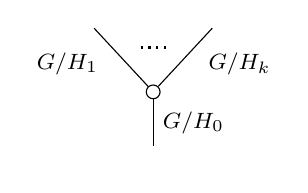
\begin{tikzpicture}
[grow=up,auto,level distance=2.3em,every node/.style = {font=\footnotesize},dummy/.style={circle,draw,inner sep=0pt,minimum size=1.75mm}]
	\node at (0,0) {}
		child{node [dummy] {}
			child{
			edge from parent node [swap,near end] {$G/H_k$} node [name=Kn] {}}
			child{
			edge from parent node [near end] {$G/H_1$}
node [name=Kone,swap] {}}
		edge from parent node [swap] {$G/H_0$}
		};
		\draw [dotted,thick] (Kone) -- (Kn) ;
\end{tikzpicture}
\]
Writing $C_n$ for the non-equivariant corolla with $n$ leaves, we note that
$C_{\amalg_i H_0/H_i} \simeq 
G \cdot_{H_0} C_{\Sigma_i |H_0/H_i|}$,
where $C_{\Sigma_i |H_0/H_i|}$ regarded as a (non-equivariant) corolla together with the obvious $H_0$-action.
\end{notation}


\begin{definition}\label{PROF DEF}
	Let $X$ be a $G$-$\infty$-operad.
	A \textit{$G$-profile} on $X$ is a map
\[
	\partial \Omega[C] \to X
\]
	for some $G$-corolla $C \in \Sigma_G$.
More explicitly, a $G$-profile is described by the following data:
\begin{itemize}
	\item subgroups $H_i \leq G$, $0\leq i \leq k$ such that
	$H_0 \geq H_i$ for $1 \leq i \leq k$;
	\item objects $x_i \in X(\eta)^{H_i}$ for $0 \leq i \leq k$.
\end{itemize}
To simplify notation, we denote a $G$-profile as 
$(x_1,\cdots,x_k;x_0)$, and refer to it as a 
\textit{$C$-profile} on $X$.
\end{definition}


\begin{definition}\label{MAPSPACESEG DEF}
Given a dendroidal Segal space $X \in \mathsf{sdSet}^G_S$
and a $C$-profile $(x_1,\cdots,x_n ; x_0)$
on $X$ 
%(defined exactly as in Definition \ref{PROF DEF})
we define the space of maps 
$X(x_1,\cdots,x_n ; x_0) \in \mathsf{sSet}$ via the pullback square
\[
\begin{tikzcd}[column sep=4em]
	X(x_1,\cdots,x_k;x_0) \ar{r} \ar{d}&
	X(\Omega[C]) \ar{d}
\\
	\Delta[0] \ar{r}[swap]{(x_1,\cdots,x_k;x_0)} &
	\prod_{0\leq i \leq k} X(\eta)^{H_i}
	\arrow[lu, phantom, "\lrcorner", very near start]
\end{tikzcd}
\]
\end{definition}

\begin{definition}\label{HMTPYGEN DEF}
	Let $X \in \mathsf{sdSet}^G$ be a dendroidal Segal space.
	The \textit{homotopy genuine operad} 
	$ho(X)\in \mathsf{dSet}_G$ is defined %
%        to be the image of $X$ under the composite
%        \begin{equation}
%              \mathsf{sdSet}^G \xrightarrow{\gamma_{\**}} \mathsf{PreOp} \into \mathsf{sdSet}^G = (\mathsf{dSet}^G)^{\Delta^{op}} \xrightarrow{u_*} = (\mathsf{dSet}_G)^{\Delta^{op}} \xrightarrow{\pi_0} \mathsf{dSet}_G,
%        \end{equation}
by
	\[
	ho(X) = \pi_0 \left( \upsilon_{\**} \left( \gamma_{\**}X \right) \right).
	\]
\end{definition}


\begin{remark}
	Writing $\iota$ for the inclusion $\Delta \to \Omega$
	and $\iota_G$ for the composite inclusion
	$\Delta \times \mathsf{O}_G \to 
	\Omega \times \mathsf{O}_G \to
	\Omega_G$,
	one has that $\iota_G^{\**}ho(X)$ is the $G$-coefficient system of categories formed by the homotopy categories
	$ho \left(\iota^{\**}\left(X^H\right)\right) = 
	\pi_0 \left(\iota^{\**} \gamma_{\**}X^H\right)$ for $H \leq G$.
\end{remark}

\begin{definition}\label{DKEQUIV DEF}
	A map $f \colon X \to Y$ of equivariant dendroidal Segal spaces is called 
\begin{itemize}
	\item \textit{fully faithful} if for all $C\in \Sigma_G$ and $C$-profile $(x_1,\cdots,x_n;x_0)$ on $X$ the map
\[
	X(x_1,\cdots,x_k;x_0) \to
	Y\left(f(x_1),\cdots,f(x_k);f(x_0)\right)
\]
is a Kan equivalence in $\mathsf{sSet}$;
	\item \textit{essentially surjective} if
	the map $\iota_G^{\**}ho(X) \to \iota_G^{\**}ho(Y)$
	is essentially surjective on all category levels of the $G$-coefficient system;
	\item a \textit{DK-equivalence} if it is both fully faithful and essentially surjective.
\end{itemize}
\end{definition}


\begin{remark}\label{ONLYPREOP REM}
Definitions \ref{MAPSPACESEG DEF}, \ref{HMTPYGEN DEF} and \ref{DKEQUIV DEF} depend only on the 
fibrant pre-operads $\gamma_{\**}X,\gamma_{\**}Y$,
since $X(x_1,\cdots,x_k;x_0) = \gamma_{\**}X(x_1,\cdots,x_k;x_0)$.
In fact, for each $G$-corolla $C$
one has a decomposition
\[
	ho(X)(C)=
%	\coprod_{\partial \Omega[C] \xrightarrow{(x_1,\cdots,x_k;x_0)} X}
	\coprod_{\text{$C$-profiles }(x_1,\cdots,x_k;x_0)}
	\pi_0 \left( X(x_1,\cdots,x_k;x_0) \right)
\]
so that, given $\varphi \in X_0(x_1,\cdots,x_k;x_0)$
we will write $[\varphi] \in ho(X)(C)$
for the corresponding class.
\end{remark}

\begin{remark}
	One can extend the previous definitions to $G$-$\infty$-operads $X,Y \in \mathsf{dSet}^G$
	by applying them to the dendroidal Segal spaces
	$X^{J^{\bullet}},Y^{J^{\bullet}} \in \mathsf{sdSet}^G$
	(cf. Remark \ref{CONCRECOM REM}). 
\end{remark}


\begin{definition}\label{HEQUIV DEF}
	Let $X\in \mathsf{sdSet}^G$ be a dendroidal Segal space.
	For $H \leq G$, we call 
	$f \in X_0(\Omega[C_{H/H}]) = X_0([1])^H$ a 
	\textit{$H$-equivalence} 
	if $[f]$ is an isomorphism in the category
	$ho\left(\iota^{\**}(X^H)\right)$.
\end{definition}

{\color{blue} add context}

Suppose $C,D \in \Sigma_G$ are $G$-corollas that can be grafted,
i.e. that $C$ has a leaf orbit and $D$ a root orbit both isomorphic to $G/H$. Denote this orbit as $G e$
and write $T= C \amalg_{G e} D$ for the grafted $G$-tree. 
For any dendroidal Segal space $X$ one then has
$X(Sc[T]) \simeq X(\Omega[C]) \times_{X(\eta)^H} X(\Omega[D])$
and one can hence choose a section in the middle row below
\begin{equation}\label{HOMOTCIRC EQ}
\begin{tikzcd}
	\{\varphi\} \times X(z_1,\cdots,z_l;e)
	\ar[dashed]{rr}{\varphi \circ_{Ge} (-)}
&&
	X(z_1,\cdots,z_l,y_2,\cdots,y_k;x)
\\
	X(\Omega[C]) \times_{X(\eta)^H} X(\Omega[D]) \ar[bend left=17,dashed]{r}
	\ar[hookleftarrow]{u}
&
	X(\Omega[T]) \ar[->>]{l}{\sim} \ar[->>]{r}
&
	X(\Omega[T-Ge])
	\ar[hookleftarrow]{u}
\\
	X(e,y_2,\cdots,y_k;x) \times \{\psi\}
	\ar[hookrightarrow]{u}
	\ar[dashed]{rr}[swap]{(-)\circ_{Ge} \psi}
&&
	X(z_1,\cdots,z_l,y_2,\cdots,y_k;x)
	\ar[hookrightarrow]{u}
\end{tikzcd}
\end{equation}
thus defining maps 
$\varphi \circ_{Ge} (-)$ (resp. $(-)\circ_{Ge} \psi$)
for any choice of 
$\varphi \in X_0(e,y_2,\cdots,y_k;x)$
(resp. $\psi \in X_0(z_1,\cdots,z_l;e)$).


\begin{remark}\label{HOMOLIFTS REM}
In what follows, we will repeatedly use the observation that, for $X\to Y$ a trivial Kan fibration, any two lifts  of the form below are homotopic.
\[
\begin{tikzcd}[row sep =1.5em]
&
	X \ar[->>]{d}{\sim}
\\
	A \ar[dashed]{ru} \ar{r}
&
	Y 
\end{tikzcd}
\]
\end{remark}


\begin{proposition}\label{GENOPHO PROP}
\begin{itemize}
	\item[(i)] the maps $\varphi \circ_{Ge} (-)$, $(-)\circ_{Ge} \psi$
are well defined up to homotopy;
	\item[(ii)] if $[\varphi]=[\bar{\varphi}]$ then 
the maps $\varphi \circ_{Ge} (-)$, $\bar{\varphi} \circ_{Ge} (-)$ are homotopic, and likewise for $[\psi] = [\bar{\psi}]$;
	\item[(iii)] $[\varphi \circ_{Ge} \psi]$
	depends only on $[\varphi]$, $[\psi]$;
	\item[(iv)] the homotopy classes of the maps $\varphi \circ_{Ge} (-)$, $(-)\circ_{Ge} \psi$ are natural with respect to maps $f\colon X \to Y$ between dendroidal Segal spaces.
\end{itemize}
\end{proposition}

\begin{proof}
	Noting that all middle row sections in \eqref{HOMOTCIRC EQ} (and homotopies between them)
	are necessarily compatible with the projections to 
$X(\partial \Omega[T-Ge])$, 
	(i) follows from Remark \ref{HOMOLIFTS REM}.
	The middle row in \eqref{HOMOTCIRC EQ}
	gives the necessary homotopies for (ii). 
	(iii) is immediate from (ii).
%For functoriality, recall that we can find a factorization 
%$X \overset{\sim}{\rightarrowtail} Z \twoheadrightarrow Y$
%as a trivial cofibration followed by a fibration in the category of dendroidal Segal spaces. Since the trivial cofibration then has a homotopy inverse, and one easily checks that so do the induced maps 
Lastly, (iv) follows from Remark \ref{HOMOLIFTS REM}
applied to the two
$X(\Omega[C]) \underset{X(\eta)^H}{\times} X(\Omega[D])
\to Y(\Omega[T])$ paths in
\[
\begin{tikzcd}[column sep =13]
	X(\Omega[T]) \ar{r} \ar[->>]{d}{\sim} &
	Y(\Omega[T]) \ar[->>]{d}{\sim}
\\
	X(\Omega[C]) \underset{X(\eta)^H}{\times} X(\Omega[D])
	\ar[bend left=30,dashed]{u} \ar{r}
&
	Y(\Omega[C]) \underset{Y(\eta)^H}{\times} Y(\Omega[D])
	\ar[bend left=30,dashed]{u}
\end{tikzcd}
\]
\end{proof}


We will now show that the operations   
$\varphi \circ_{Ge} (-)$, $(-)\circ_{Ge} \psi$
satisfy the obvious compatibilities one expects, but we will find it convenient to first package these compatibilities into a common format. In the categorical case (corresponding to linear trees), there are three types of ``associativity'' compatibilities, corresponding to homotopies
\[
	\varphi \circ \left( \psi \circ (-) \right)
		\sim
	(\varphi \circ \psi) \circ (-) 
\qquad
	\varphi \circ \left( (-)  \circ \psi \right)
		\sim
	\left( \varphi \circ (-) \right) \circ \psi 
\qquad
	\left( (-) \circ \varphi \right) \circ \psi 
		\sim
	(-) \circ (\varphi \circ \psi) 
\]	
but in the operadic case there are instead five cases, corresponding to the different possible roles of the nodes in 
$G$-trees $T$ with exactly three $G$-vertices, whose \textit{orbital} representation falls into one of the two cases illustrated below.
\[%
	\begin{tikzpicture}[auto,grow=up, every node/.style = {font=\scriptsize,inner sep=1pt},
	dummy/.style = {circle,draw,inner sep=0pt,minimum size=1.75mm}]%
	\begin{scope}[level distance = 1.6em]
	\tikzstyle{level 2}=[sibling distance=4em]%
	\tikzstyle{level 3}=[sibling distance=2em]%
	\tikzstyle{level 4}=[sibling distance=1em]%
		\node at (0,0) [font=\normalsize]{$T$}%
			child{node [dummy] {}%
				child[level distance = 1.5em]{node {}}%
				child[level distance = 2.2em]{node [dummy] {}%
					child[level distance = 1.3em]{}%
					child[level distance = 2.2em,sibling distance=1.4em]{node [dummy] {}
						child[level distance = 1.6em]
						child[level distance = 1.6em]
					edge from parent node [swap,very near end] {$Gf$}}%
					child[level distance = 2.2em,sibling distance=1.4em]{}%
					child[level distance = 1.3em]{}%
				edge from parent node [swap]{$Ge$}}%
				child[level distance = 1.5em]{node {}}%
			};%
	\end{scope}
	\begin{scope}[level distance = 1.7em]
	\tikzstyle{level 2}=[sibling distance=2.75em]%
	\tikzstyle{level 3}=[sibling distance=1.25em]%
		\node at (8,0) [font=\normalsize] {$T$}%
			child{node [dummy] {}%
				child[level distance = 1.2em]{node {}}%
				child[sibling distance=2em,level distance = 2.2em]{node [dummy] {}%
					child[level distance = 1.6em]{}%
					child[level distance = 1.8em]{}%
					child[level distance = 1.6em]{}%
				edge from parent node [swap,near end] {$Gf$}}%
				child[sibling distance=2em,level distance = 2.2em]{}%
				child[level distance = 1.2em]{node [dummy] {}%
					child[level distance = 1.6em]{}%
					child[level distance = 1.6em]{}%
				edge from parent node {$Ge$}}%
			};%
	\end{scope}
	\end{tikzpicture}%
\]%
Since all these compatibilities can be simultaneously encoded in terms of such trees, we will simply refer to all types of compatibility simply as \textit{associativity}.
As noted pictorially above, such a $G$-tree $T$
has exactly two inner edge orbits $Ge$ and $Gf$.
In the next result, we write $T[Ge]$ (resp. $T[Gf]$) for the orbital outer face of $T$ with $Ge$ (resp. $Gf$) as its single inner edge orbit. 
\[%
	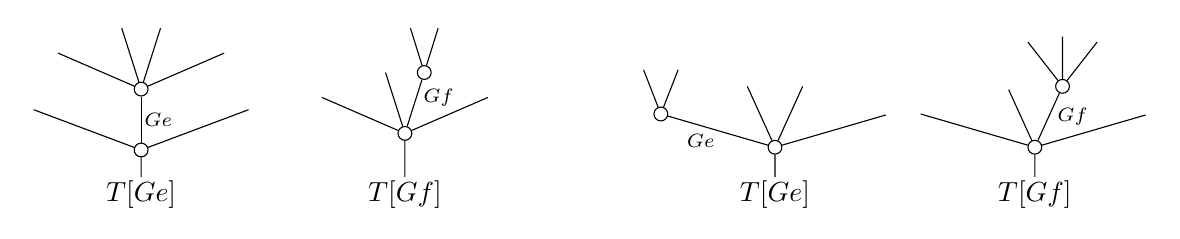
\begin{tikzpicture}[auto,grow=up, every node/.style = {font=\scriptsize,inner sep=1pt},
	dummy/.style = {circle,draw,inner sep=0pt,minimum size=1.75mm}]%
	\begin{scope}[level distance = 1.6em]
	\tikzstyle{level 2}=[sibling distance=4em]%
	\tikzstyle{level 3}=[sibling distance=2em]%
	\tikzstyle{level 4}=[sibling distance=1em]%
		\node at (-1.675,0) [font=\normalsize]{$T[Ge]$}%
			child{node [dummy] {}%
				child[level distance = 1.5em]{node {}}%
				child[level distance = 2.2em]{node [dummy] {}%
					child[level distance = 1.3em]{}%
					child[level distance = 2.2em,sibling distance=1.4em]{
					}%
					child[level distance = 2.2em,sibling distance=1.4em]{}%
					child[level distance = 1.3em]{}%
				edge from parent node [swap]{$Ge$}}%
				child[level distance = 1.5em]{node {}}%
			};%
	\end{scope}
	\begin{scope}[level distance = 1.6em]
	\tikzstyle{level 2}=[sibling distance=2em]%
	\tikzstyle{level 3}=[sibling distance=1em]%
		\node at (1.675,0) [font=\normalsize]{$T[Gf]$}%
			child[level distance = 2.2em]{node [dummy] {}%
				child[level distance = 1.3em]{}%
				child[level distance = 2.2em,sibling distance=1.4em]{node [dummy] {}
					child[level distance = 1.6em]
					child[level distance = 1.6em]
				edge from parent node [swap,very near end] {$Gf$}}%
				child[level distance = 2.2em,sibling distance=1.4em]{}%
				child[level distance = 1.3em]{}%
			};%
	\end{scope}
	\begin{scope}[level distance = 1.7em]
	\tikzstyle{level 2}=[sibling distance=2.75em]%
	\tikzstyle{level 3}=[sibling distance=1.25em]%
		\node at (6.375,0) [font=\normalsize] {$T[Ge]$}%
			child{node [dummy] {}%
				child[level distance = 1.2em]{node {}}%
				child[sibling distance=2em,level distance = 2.2em]{
				}%
				child[sibling distance=2em,level distance = 2.2em]{}%
				child[level distance = 1.2em]{node [dummy] {}%
					child[level distance = 1.6em]{}%
					child[level distance = 1.6em]{}%
				edge from parent node {$Ge$}}%
			};%
		\node at (9.675,0) [font=\normalsize] {$T[Gf]$}%
			child{node [dummy] {}%
				child[level distance = 1.2em]{node {}}%
				child[sibling distance=2em,level distance = 2.2em]{node [dummy] {}%
					child[level distance = 1.6em]{}%
					child[level distance = 1.8em]{}%
					child[level distance = 1.6em]{}%
				edge from parent node [swap,near end] {$Gf$}}%
				child[sibling distance=2em,level distance = 2.2em]{node {}}%
				child[level distance = 1.2em]{
				}%
			};%
	\end{scope}
	\end{tikzpicture}%
\]%


\begin{proposition}\label{ASSOC PROP}
	The operations
	$\varphi \circ_{Ge} (-)$, $(-)\circ_{Ge} \psi$
	satisfy all associativity conditions with respect to 
	$G$-trees with three $G$-vertices.
	Further, if $C=C_{H/H}$ and $\varphi = s(e)$ is the degeneracy on $e$, then $\varphi \circ_{Ge} (-)$ is homotopic to the identity, and similarly for 
	$D=C_{H/H}$ and $\varphi = s(e)$.
\end{proposition}


\begin{proof}
We abbreviate
$Sc_{T[Ge]}[T] =
Sc[T] \amalg_{Sc[T[Ge]]} \Omega[T[Ge]] =
Sc[T] \amalg_{\Lambda^{Ge}_o[T[Ge]]} \Omega[T[Ge]]$,
which can be regarded as the union
$Sc[T] \cup \Omega[T[Ge]]$
of subcomplexes of $\Omega[T]$.
We now consider the following diagram, 
where all solid maps are Kan fibrations, 
and the maps labelled $\sim$ are trivial Kan fibrations
($Sc_{T[Ge]}[T]$ is a cover in the sense of Remark \ref{RECOVER REM}(i),
hence both maps $Sc[T] \to Sc_{T[Ge]}[T] \to \Omega[T]$ are $G$-inner anodyne), so that one can choose the indicated sections.
\begin{equation}\label{FOURSQ EQ}
\begin{tikzcd}[column sep = 2.5em,row sep = 2.5em]
	X(Sc[T]) 
	\ar[bend left=17,dashed]{r}
	\ar[bend right=30,dashed]{d}&
	X(Sc_{T[Ge]}[T])
	 \ar[->>]{l}{\sim} \ar[->>]{r} 
	\ar[bend right=30,dashed]{d}&
	X(Sc[T-Ge])
	\ar[bend right=30,dashed]{d}
\\
	X(Sc_{T[Gf]}[T]) \ar[->>]{u}[swap]{\sim} \ar[->>]{d}
	\ar[bend left=17,dashed]{r}& 
	X(\Omega[T]) \ar[->>]{l}{\sim} \ar[->>]{u}[swap]{\sim} \ar[->>]{r} 
	\ar[->>]{d}&
	X(\Omega[T-Ge]) \ar[->>]{u}[swap]{\sim} \ar[->>]{d}
\\
	X(Sc[T-Gf]) 
	\ar[bend left=17,dashed]{r}&
	X(\Omega[T-Gf]) \ar[->>]{r} \ar[->>]{l}{\sim}&
	X(\Omega[T-Ge-Gf])
\end{tikzcd}
\end{equation}
But since the desired associativity conditions amount to the claim that the top right and left bottom composites 
$X(Sc[T]) \to X(\Omega[T-Ge-Gf])$
are homotopic, the associativity result follows from Remark \ref{HOMOLIFTS REM}.
For the ``further'' claim, note that by Remark \ref{HOMOLIFTS REM} one is free to modify \eqref{HOMOTCIRC EQ} so as to use any lift of the form below.
But then since the $G$-tree $T$ is degenerate on the $G$-corolla $D$, such a lift is given by the degeneracy operator and the result follows.
\[
\begin{tikzcd}[row sep =1.5em]
&
	X(\Omega[T]) \ar[->>]{d}{\sim}
\\
	\{s(e)\} \times X(z_1,\cdots,z_l;e) \ar[dashed]{ru} \ar{r}
&
	X(Sc[T])
\end{tikzcd}
\]
%Noting that the following three diagrams,
%where $\Lambda_o^{Ge,Gf}[T]$ is a generalized orbital $G$-horn
%and $\Lambda_{o,c}^{Ge}[T]$, $\Lambda_{o,c}^{Gf}[T]$
%are characteristic orbital $G$-horns (cf. {\color{red} ref}), are pullbacks
%\[
%\begin{tikzcd}[column sep =12]
%	X(\mathsf{Sc}[T]) 
%	\arrow[rd, phantom, "\ulcorner", near start]& 
%	X(\mathsf{Sc}_{T[Ge]}[T])
%	\ar[->>]{l}{\sim}
%&
%	X(\mathsf{Sc}_{T[Ge]}[T])
%	\ar[->>]{r} &
%	X(\mathsf{Sc}[T-Ge])
%	\arrow[ld, phantom, "\urcorner", near start]
%&
%	X(\mathsf{Sc}_{T[Gf]}[T])  \ar[->>]{d}
%	& 
%	X(\Lambda_{o,c}^{Ge}[T]) \ar[->>]{l}{\sim}  \ar[->>]{d}
%\\
%	X(\mathsf{Sc}_{T[Gf]}[T]) \ar[->>]{u}[swap]{\sim} &
%	X(\Lambda_o^{Ge,Gf}[T]) \ar[->>]{u}[swap]{\sim}
%	\ar[->>]{l}{\sim}
%&
%	X(\Lambda_{o,c}^{Gf}[T]) \ar[->>]{u}[swap]{\sim}
%	\ar[->>]{r} &
%	X(\Omega[T-Ge]) \ar[->>]{u}[swap]{\sim}
%&
%	X(\mathsf{Sc}[T-Gf]) 
%	\arrow[ur, phantom, "\llcorner", near start]
%	&
%	X(\Omega[T-Gf]) \ar[->>]{l}{\sim}&
%\end{tikzcd}
%\]
%one sees that:
%\begin{inparaenum}
%	\item[(i)] sections in the top left square of \eqref{FOURSQ EQ} can be chosen to be compatible in the sense that the two composites
%$X(Sc[T]) \to X(\Omega[T])$ coincide;
%	\item[(ii)] 
%	sections in the top right and bottom left squares of \eqref{FOURSQ EQ} can be chosen to be compatible in the sense that the two composites
%$X(Sc[T-Ge]) \to X(\Omega[T])$ and $X(Sc[T-Gf]) \to X(\Omega[T])$ coincide.
%\end{inparaenum}
%Note that we do not claim (or need) that (i) and (ii) hold simultaneously.
%We thus conclude that the possible choices of maps 
%$X(\mathsf{Sc}[T]) \to X(\Omega[T-Ge-Gf])$
%given by outer paths in \eqref{FOURSQ EQ}
%are homotopic. All desired forms of associativity follow from taking fibers of these maps over the objects $X(\partial \Omega[T-Ge-Gf])$.
\end{proof}


\begin{remark}
	In the non-equivariant case the associativity and unit conditions in the previous result capture all the key compatibilities of the
	$\varphi \circ_{e} (-)$, $(-)\circ_{e} \psi$
	operations.
	However, in the equivariant case there are further 
	``compatibilities with pullback of $G$-trees'', which are closely related to the genuine equivariant operads introduced in \cite{BP17}. 
	Nonetheless, describing these extra compatibilities would require using $G$-trees with more than three $G$-vertices, and since such compatibilites are not needed for our present goals, we omit their discussion. 
\end{remark}


%\begin{corollary}
%DK-equivalences between dendroidal Segal spaces satisfy 2-out-of-3.
%\[
%\begin{tikzcd}[row sep =5]
%	X \ar{rr}{gf} \ar{rd}[swap]{f} && Z \\
%	& Y \ar{ru}[swap]{g}
%\end{tikzcd}
%\]
%\end{corollary}

%\begin{proof}
%The non trivial claim is that when $f$ and $gf$ are DK-equivalences then so is $g$, or more precisely, that the maps
%\[
%	Y(y_1,\cdots,y_n;y_0)
%\to
%	Z(g(y_1),\cdots, g(y_n); g(y_0))
%\]
%are weak equivalences even if the $y_i$ are not in the image of $f$.
%But this follows from the functoriality in 
%Proposition \ref{GENOPHO PROP},
%essential surjectivity 
%(note that when $y_i \in Y(\eta)^{H_i}$ one needs to use $H_i$-equivalences), 
%and the fact that by Proposition \ref{ASSOC PROP} the maps
%$f \circ_{Ge} (-)$, $(-)\circ_{Ge} f$
%are weak equivalences whenever $f$ is a $H$-equivalence.
%\end{proof}

\begin{corollary}\label{26COR}
DK-equivalences between dendroidal Segal spaces satisfy 2-out-of-6, i.e. when in
$X \xrightarrow{f} 
Y \xrightarrow{g}
Z \xrightarrow{h} W$ the maps
$gf$ and $hg$ are DK-equivalences then so are
$f$, $g$, $h$, $hgf$.
\end{corollary}

\begin{proof}
Applying the 2-out-of-6 properties in $\mathsf{sSet}$ and $\mathsf{Cat}$ to mapping spaces and homotopy categories $\iota_G^{\**}ho$,
the only non obvious conditions are the fully faithfulness of $g,h$ for $C$-profiles not in the image of $f$. 
But since by Proposition \ref{ASSOC PROP} the maps
$f \circ_{Ge} (-)$, $(-)\circ_{Ge} f$
are weak equivalences when $f$ is a $H$-equivalence,
this last claim follows from essential surjectivity.
\end{proof}


The following roughly summarizes (and slightly refines)
\cite[Lemma 5.8, Theorem 6.2, Prop. 11.1, Lemma 11.10]{Rez01} in our setup.


\begin{proposition}\label{SESP PROP}
	Let $X \in \mathsf{ssSet}$ be a Segal space. Then:
\begin{itemize}
	\item[(i)] equivalences of $X$ define a subset of connected components
	$X^h(1) \subset X(1)$;
	\item [(ii)] the pullbacks
\begin{equation}\label{XHDEF EQ}
\begin{tikzcd}[row sep=1.5em]
	X^h(n) \ar{r} \ar{d} & X(n) \ar{d}
\\
	X^h(1) \times_{X(0)} \cdots \times_{X(0)} X^h(1) \ar{r} &
	X(1) \times_{X(0)} \cdots \times_{X(0)} X(1)
	\arrow[lu, phantom, "\lrcorner", very near start]
\end{tikzcd}
\end{equation}
define a Segal space $X^h \subset X$, consisting of a union of connected components at each level;
	\item[(iii)] the maps
	$X^h(2) \xrightarrow{(d_2,d_1)}
	X^h(\Lambda^0[2])$, 
	$X^h(2) \xrightarrow{(d_0,d_1)} 
	X^h(\Lambda^2[2])$
	are trivial fibrations;
	\item[(iv)] the map $X(J) \to X({\Delta[1]}) = X(1)$ factors through a weak equivalence $X(J) \to X^h(1)$.
\end{itemize}
\end{proposition}


\begin{proof}
For (i), given 
$f \colon x \to y$ in $X_0(1)$
then $[f]$ has a left inverse iff there exists $p$
as on the left diagram below. But for any path $H$ between $f$ and $f'$ in $X(1)$ there is a lift in the right diagram
\[
\begin{tikzcd}[column sep =40]
	& X(2) \ar[->>]{d}{(d_2,d_1)}
&
	\Delta[0] \ar{r}{p} \ar{d}[swap]{0} &
	X(2) \ar[->>]{d}{(d_2,d_1)}
\\
	\Delta[0] \ar{r}[swap]{(f,s_0(x))} \ar{ru}{p} &
	X(1) \times_{X(0)} X(1)
&
	\Delta[1] \ar{r}[swap]{(H,s_0 d_1(H))} \ar[dashed]{ru} &
	X(1) \times_{X(0)} X(1)
\end{tikzcd}
\]
showing that $f'$ is also left-invertible. The situation for right inverses is identical, thus (i) follows.

For (ii), that $X^h$ is closed under the simplicial operators follows equivalences are closed under composition.
Moreover, noting that \eqref{XHDEF EQ} can be reinterpreted
as on the left below,
cellular induction induces the right pullbacks for all 
$K\in \mathsf{sSet}$.
\[
\begin{tikzcd}[row sep=1.5em]
	X^h(\Delta[n]) \ar{r} \ar{d} &
	X(\Delta[n]) \ar{d}
&&
	X^h(K) \ar{r} \ar{d} &
	X(K) \ar{d}
\\
	X^h(\mathsf{sk}_1 \Delta[n]) \ar{r} &
	X(\mathsf{sk}_1 \Delta[n])
	\arrow[lu, phantom, "\lrcorner", very near start]
&&
	X^h(\mathsf{sk}_1 K) \ar{r} &
	X(\mathsf{sk}_1 K)
	\arrow[lu, phantom, "\lrcorner", very near start]
\end{tikzcd}
\]
Since 
$\mathsf{sk}_1 (\partial \Delta[n]) = 
\mathsf{sk}_1 \Delta[n]$
if $n \geq 2$
it follows that the maps
$X^h(n) \to X^h(\partial \Delta[n])$, $n\geq 2$
are Kan fibrations, and since the map $X^h(1)\ \to X(0) \times X(0)$
is certainly a Kan fibration, $X^h$ is indeed Reedy fibrant. 
The Segal condition is obvious from the pullback \eqref{XHDEF EQ}.

For (iii), it suffices by symmetry to establish the first claim.
It is then enough to show that for any choice of section 
in the following diagram the top composite is a Kan equivalence.
\[
\begin{tikzcd}[column sep = 60]
	X^h(1) \times_{X_0} X^h(1) \ar[bend left=17,dashed]{r} 
	\ar[->>]{rd}[swap]{(id,d_0)}&
	X^h(2) \ar[->>]{r}[swap]{(d_2,d_1)} \ar[->>]{l}{(d_2,d_0)}[swap]{\sim}&
	X^h(1) \times_{X_0} X^h(1)
	\ar[->>]{dl}{(id,d_0)}
\\
	& X^h(1) \times X(0)
\end{tikzcd}
\]
But this composite is a map of fibrations over
$X^h(1) \times X(0)$ with the map between the fibers over 
$(f \colon x \to y,z)$
computing the map
$(-) \circ f \colon X^h(y;z) \to X^h(x;z)$,
which is a Kan equivalence since $f \in X^h(1)$ is an equivalence.
Thus the composite is a Kan equivalence, establishing (iii).


Lastly, for (iv) note that (iii) says that $X^h$ is local with respect to the outer horn inclusions
$\Lambda^0[2] \to \Delta[2]$ and
$\Lambda^2[2] \to \Delta[2]$, 
and hence by Remarks 
\ref{ANHYPER REM} and \ref{CONTGR REM}
the map 
$X^h(J) \to X^h(1)$ 
is a Kan equivalence.
The only remaining claim is that
$X^h(J) = X(J)$, which is clear.
\end{proof}

\begin{remark}
The proof of (ii) shows that the inclusion $X^h \to X$ is a Reedy fibration.
\end{remark}

\subsection{Rezk completion and fibrant Segal operads}


In the next result we make use of a decomposition of the tensor product $[1] \otimes C$,
where $[1]$ is the $1$-simplex regarded as a $G$-trivial $G$-tree, and $C$ is a $G$-corolla 
(see Notation \ref{GCOR NOT}). Slightly adapting the discussion
in Example \ref{THM71 EX}, $[1] \otimes C$ is the union of two maximal $G$-subtrees $C \star \eta$ and $\eta \star C$,
whose orbital representations are depicted below.
\[
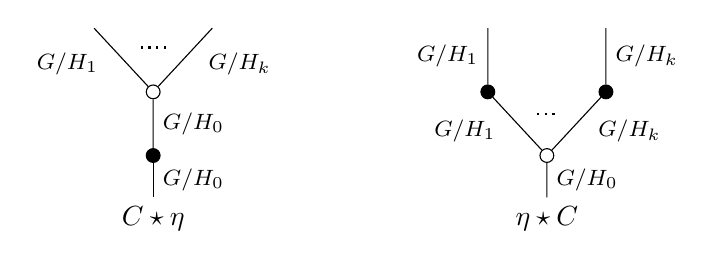
\begin{tikzpicture}
[grow=up,auto,level distance=2.3em,every node/.style = {font=\footnotesize},dummy/.style={circle,draw,inner sep=0pt,minimum size=1.75mm}]
	\node at (0,0) [font=\normalsize] {$C \star \eta$}
		child{node [dummy,fill=black] {}
			child{node [dummy] {}
				child{
				edge from parent node [swap,near end] {$G/H_k$} node [name=Kn] {}}
				child{
				edge from parent node [near end] {$G/H_1$}
node [name=Kone,swap] {}}
			edge from parent node [swap] {$G/H_0$}}
		edge from parent node [swap] {$G/H_0$}};
		\draw [dotted,thick] (Kone) -- (Kn) ;
	\node at (5,0) [font=\normalsize] {$\eta \star C$}
		child{node [dummy] {}
			child{node [dummy,fill=black] {}
				child{
				edge from parent node [swap] {$G/H_k$}}
			edge from parent node [swap,near end] {$G/H_k$} node [name=Kn] {}}
			child{node [dummy,fill=black] {}
				child{
				edge from parent node {$G/H_1$}}
			edge from parent node [near end] {$G/H_1$}
node [name=Kone,swap] {}}
		edge from parent node [swap] {$G/H_0$}
		};
		\draw [dotted,thick] (Kone) -- (Kn) ;
\end{tikzpicture}
\]
Moreover, much as in \eqref{GENLEXREL EQ}, 
$C \star \eta$ and $\eta \star C$ have a common orbital face, which we denote simply as $C$
(this face is canonically isomorphic to the original $C$),
leading to a decomposition
\[
\Omega[1] \otimes \Omega[C]
	\simeq
\Omega[C \star \eta] \otimes_{\Omega[C]} \Omega[\eta \star C]
\]
We note that this holds even if $k=0$, 
which is an exceptional case since then
$[1] \otimes C = C \star \eta$.



\begin{proposition}\label{JDDK PROP}
	Let $X\in \mathsf{sdSet}^G$ be a dendroidal Segal space. 
	Then the map $X \to X^{J}$ is a $DK$-equivalence.
\end{proposition}


\begin{proof}
	Note first that for any $T \in \Omega_G$ the map
	$X^{J}(T) \to X^{\Omega[1]}(T)$ can be rewritten as
	$\left(X^{\Omega[T]}\right)(J) \to
	\left(X^{\Omega[T]}\right)(\Omega[1])
%	= \left(\iota^{\**}\left(X^{\Omega[T]}\right)\right)(1)
	$,
	and since $\iota^{\**}\left( X^{\Omega[T]} \right)$
	is a (simplicial) Segal space
	Proposition \ref{SESP PROP}(iv) says that this map is 
	a weak equivalence onto a subset of components,
	i.e. a \textit{homotopy monomorphism}.
	Hence, for any $G$-corolla
	$C=C_{\amalg_i H_0/H_i}$ the horizontal maps in 
	the right square below are homotopy monomorphisms.
\begin{equation}\label{BIGSQ EQ}
\begin{tikzcd}
	X(C) \ar{r} \ar[->>]{d} & 
	X^{J}(C) \ar{r} \ar[->>]{d} & 
	X^{\Omega[1]}(C) \ar[->>]{d}
\\
	\prod_{0\leq i\leq k} X(\eta)^{H_i} \ar{r}&
	\prod_{0\leq i\leq k} \left(X^{J}(\eta)\right)^{H_i} \ar{r} &
	\prod_{0\leq i\leq k} \left(X^{\Omega[1]}(\eta)\right)^{H_i}
\end{tikzcd}	
\end{equation}

Since fully faithfulness of $X \to X^{J}$
is the statement that the leftmost square in \eqref{BIGSQ EQ} induces weak equivalences on fibers, it suffices to show that so does the composite square.

Now note that
$X^{\Omega[1]}(C) = X\left(\Omega[1] \otimes \Omega[C]\right)$ and that there is a pullback diagram as on the left below. Moreover, both squares below are pullback squares which are injective fibrant squares
and the natural map of squares between them is an injective fibration of squares (alternatively, the fibrancy claims state that the resulting cube is an injective fibrant cube).
\begin{equation}\label{OTBIGSQ EQ}
\begin{tikzcd}[column sep=14]	
	X\left(\Omega[1] \otimes \Omega[C]\right)
	\ar[->>]{r} \ar[->>]{d}&
	X(\Omega[\eta \star C]) \ar[->>]{d}
&
	\underset{i}{\prod} X([1])^{H_i} \ar[->>]{r} \ar[->>]{d} &
	\left(\underset{i \neq 0}{\prod} X([1])^{H_i}\right)
	\times X(\eta)^{H_0} \ar[->>]{d}
\\
	X(\Omega[C \star \eta])	 \ar[->>]{r} &
	X(\Omega[C])
&
	\left(\underset{i \neq 0}{\prod} X(\eta)^{H_i}\right)
	\times X([1])^{H_0}	 \ar[->>]{r} &
	\underset{i}{\prod} X(\eta)^{H_i}
\end{tikzcd}
\end{equation}
Since the top left corner of the map of squares 
\eqref{OTBIGSQ EQ} is the right vertical map in \eqref{BIGSQ EQ},
and noting that fibers (in the category of square diagrams)
of a fibration between pullback squares are a fibrant pullback square,
the desire claim that the total diagram in \eqref{BIGSQ EQ}
induces equivalences on fibers will follow provided that the same holds for the following squares.
\[
\begin{tikzcd}[column sep=17]
	X(\Omega[C]) \ar{r}{s_{\eta}} \ar[->>]{dd}&
	X(\Omega[C \star \eta]) \ar[->>]{d}{\sim}
&
	X(\Omega[C]) \ar{r}{s_{\eta}} \ar[->>]{dd}&
	X(\Omega[\eta \star C]) \ar[->>]{d}{\sim}
\\
	& X(\Omega[C]) \underset{X(\eta)^{H_0}}{\times} X([1])^{H_0} \ar[->>]{d}
&
	& \underset{i \neq 0}{\prod} X([1])^{H_i} 
	\underset{\underset{i \neq 0}{\prod} X(\eta)^{H_i}}{\times} X(\Omega[C]) \ar[->>]{d}
\\
	\underset{i}{\prod} X(\eta)^{H_i} \ar{r}[swap]{s_0} &
	\left(\underset{i \neq 0}{\prod} X(\eta)^{H_i}\right)
	\times X([1])^{H_0}
&
	\underset{i}{\prod} X(\eta)^{H_i} \ar{r}[swap]{s_0} &
	\left(\underset{i \neq 0}{\prod} X([1])^{H_i}\right)
	\times X(\eta)^{H_0}
\end{tikzcd}
\]
But this is clear from the fact that the top right vertical
maps in these diagrams are trivial Kan fibrations
thanks to the Segal condition.

Lastly, to check essential surjectivity, 
since $G$ acts trivially on $J$ one has
$\left(\iota_G^{\**}\left( X^J \right)\right)(G/H)=
\left(\iota_G^{\**}\left( X \right)(G/H)\right)^J$
so that we reduce to the case of $X$ a (simplicial) Segal space.
Noting that $J$ is a contractible Kan complex,
one has a map 
$H \colon J \times J \to \{0\} \times J$
such that 
$H|_{\{0\}\times J} = id_{\{0\} \times J}$
and
$H|_{\{1\}\times J} = (0,0)$.
But noting that 
$X(J \times J) \to X(\{0\} \times J)$
can be written as 
$X^J(0) \to X^J(J)$, the composite below
shows that any object in $\left(X^J\right)_0$ is indeed equivalent to a 
degenerate object, which is thus in the image of $X\to X^J$.
\[
	X^J(0) \xrightarrow{X(H)} 
	X^{J}(J) \to
	X^J(1) \rightrightarrows X^J(0)
\]
%
%\[	
%\begin{tikzcd}[column sep =12]
%	X^{\Omega[1] \otimes \Omega[C]} \ar[->>]{r}{\sim} \ar[->>]{d}[swap]{\sim} &
%	\bullet \ar[->>]{d}[swap]{\sim} \ar[->>]{r} &
%	X(C \star \eta) \ar[->>]{d}[swap]{\sim}
%\\
%	\bullet \ar[->>]{r}{\sim} \ar[->>]{d} & 
%	\underset{1 \leq i \leq n}{\prod} X([1])^{H_i} 
%	\times_{\underset{1 \leq i \leq n}{\prod} X(\eta)^{H_i}}
%	X(C)
%	\times_{X(\eta)^{H_0}} X([1])^{H_0} \ar[->>]{d}
%	\ar[->>]{r} &
%	X(C) \times_{X(\eta)^{H_0}} X([1])^{H_0} \ar[->>]{d}
%\\
%	X(\eta \star C) \ar[->>]{r}{\sim} \ar[->>]{r} &
%	\underset{1 \leq i \leq n}{\prod} X([1])^{H_i} 
%	\times_{\underset{1 \leq i \leq n}{\prod} X(\eta)^{H_i}}
%	X(C) \ar[->>]{r}
%	&
%	X(C)
%\end{tikzcd}	
%\]
\end{proof}


\begin{definition}
	Two maps $f,f'\colon A \rightrightarrows B$ between dendroidal Segal spaces are called $J$-homotopic, written $f \sim_J f'$, if
	there is a $H$ such that
	the two composites
	$A \xrightarrow{H} B^J \rightrightarrows B$
	are $f,f'$.
	
	Further, a map $f\colon X \to Y$ of dendroidal Segal spaces is called a $J$-homotopy equivalence if there exists $g \colon Y \to X$
	such that $gf \sim_J id_X$, $fg \sim_J id_Y$.
\end{definition}

\begin{remark}
	For $f\sim_J f'$, Proposition \ref{JDDK PROP} and 2-out-of-3 applied to $A \xrightarrow{H} B^J \rightrightarrows B$ imply that $f$ is a DK-equivalence iff $f'$ is.
	Thus by 2-out-of-6 $J$-homotopy equivalences are DK-equivalences.
\end{remark}


\begin{remark}\label{ALLXJK REM}
	Let $X$ be a dendroidal Segal space. All simplicial operators
	$X^{J^m} \to X^{J^{m'}}$ are induced by equivalences of groupoids $\widetilde{[m']} \to \widetilde{[m]}$,
	and are thus $J$-homotopy equivalences and thus also DK-equivalences.
\end{remark}


\begin{proposition}\label{COMPLE PROP}
Let $X \in \mathsf{sdSet}^G$ be a dendroidal Segal space. 
Then there is a complete dendroidal Segal space $\tilde{X}$
and complete equivalence $X \to \tilde{X}$ such that
\begin{itemize}
	\item[(i)] $X \to \tilde{X}$ is a monomorphism and a DK-equivalence;
	\item[(ii)] $X_0(\eta) \to \tilde{X}_0(\eta)$ is an isomorphism.
\end{itemize}
\end{proposition}


\begin{proof}
Our proof mostly adapts the construction of the completion functor in \cite[\S 10.4]{Rez01}.

Firstly, we let 
$X^{J^{\bullet}} \in (\mathsf{sdSet}^G)^{\Delta^{op}}
= \mathsf{ssdSet}^G$
be the object whose $m$-th level
is $X^{J^m}$.

We will regard the new simplicial direction in $\mathsf{ssdSet}^G=(\mathsf{sdSet}^G)^{\Delta^{op}}$ as horizontal and the old one as vertical, and abbreviate the Reedy model structure on $(\mathsf{sdSet}^G)^{\Delta^{op}}$
with respect to the dendroidal Reedy model structure on 
$\mathsf{sdSet}^G$
as the \textit{horizontal Reedy model structure} on 
$\mathsf{ssdSet}^G$.

Noting that $J^{\bullet}$ is a Reedy cofibrant cosimplicial object, it follows that 
$X^{J^{\bullet}}$ is horizontal Reedy fibrant, and it is thus formal that  
$X^{J^{\bullet}} \to \mathsf{csk}_{\eta} X^{J^{\bullet}}$
is a horizontal fibration in $(\mathsf{sdSet}^G)^{\Delta^{op}}$ as well.
As such, for $T \in \Omega_G$
the evaluations 
\begin{equation}\label{MOREOVER EQ}
X^{J^{\bullet}}(\Omega[T]) \to
\left(\mathsf{csk}_{\eta}X^{J^{\bullet}}\right)(\Omega[T])
\end{equation}
are horizontal Reedy fibrations in $\mathsf{ssSet}$
in the sense of in \S \ref{JOINBOUS SEC}.
In particular, for each vertex map $[0] \to [m]$ the induced square
\[
\begin{tikzcd}
	X^{J^m}(\Omega[T]) \ar[->>]{r} \ar[->>]{d}&
	X(\Omega[T]) \ar[->>]{d}
\\
	\underset{e_i \in E_G(T)} {\prod} \left(X^{J^m}(\eta)\right)^{H_i} \ar[->>]{r} &
	\underset{e_i \in E_G(T)} {\prod} \left(X(\eta)\right)^{H_i}
\end{tikzcd}
\]
is an (injective) fibrant square, which by Remark \ref{ALLXJK REM}
induces weak equivalences on fibers,
so that the map from $X^{J^m}(\Omega[T])$ to the pullback of the remaining diagram is a trivial Kan fibration.

By (the dual of) Remark \ref{HYPERSIMPL REM} we have just shown that \eqref{MOREOVER EQ}
satisfies the ``moreover'' condition in 
Corollary \ref{SSETSSETADJ COR}. Therefore, applying $\delta^{\**}$ to \eqref{MOREOVER EQ} yields a Kan fibration, so that all fibers of
$\delta^{\**}\left(X^{J^{\bullet}}(\Omega[T])\right) \to
\delta^{\**}\left(\left(\mathsf{csk}_{\eta}X^{J^{\bullet}}\right)(\Omega[T])\right)$
are in fact homotopy fibers.

We now write $\tilde{X}$ for a dendroidal Reedy fibrant replacement of the diagonal 
$\delta^{\**} \left(X^{J^{\bullet}}\right) \in \mathsf{sdSet}^G$,
which we note can always be chosen so that
$\delta^{\**} \left(X^{J^{\bullet}}\right) \to \tilde{X}$
is a monomorphism and
$\tilde{X}_0(\eta) = 
\left(\delta^{\**} \left(X^{J^{\bullet}}\right)\right)_0(\eta)=
X_0(\eta)$ (this follows since fibrant replacements in the Kan model structure in $\mathsf{sSet}$ can be chosen to preserve $0$-simplices, since existence of lifts against the horn inclusions
$\Delta[0]=\Lambda^0[1]\to \Delta[1]$,
$\Delta[0]=\Lambda^1[1]\to \Delta[1]$
is automatic).

To see that $\tilde{X}$ is a complete Segal space, note that in the composite
$X_0^{J^{\bullet}} \to
\delta^{\**}\left( X^{J^{\bullet}} \right)
\to \tilde{X}$
the first map is a dendroidal Reedy equivalence by Proposition \ref{SSSETJREE PROP}(iv) and the second by definition of $\tilde{X}$.
But since $X_0^{J^{\bullet}}$ is a complete Segal space by Remark \ref{CONCRECOM REM}, so is $\tilde{X}$.

For the remaining claim that the composite
$X = X^{J^{0}} \to 
\delta^{\**}\left( X^{J_{\bullet}} \right)
\to \tilde{X}$
is a DK equivalence, 
note that though
the first map is no longer a dendroidal Reedy equivalence, 
it is nonetheless an equivalence
on fibers over
$\prod_{e_i \in E_G(T)} \left(X(\eta)\right)^{H_i}$
for each $T\in \Omega_G$.
And since we have shown that the fibers of
$\delta^{\**}\left( X^{J^{\bullet}} \right)(T)$
 are homotopy fibers, these are equivalent to the fibers of $\tilde{X}(T)$ (since Reedy replacement does not change the homotopy fibers), and thus $X \to \tilde{X}$ is indeed fully faithful.
Essential surjectivity is trivial since the objects coincide.
The monomorphism condition is clear.
\end{proof}


\begin{theorem}\label{COMPIFFDK THM}
	A map of $X \to Y$ of dendroidal Segal spaces is a complete equivalence iff it is a DK-equivalence.
\end{theorem}


\begin{proof}
By the previous result one is free to assume that $X,Y$ are complete, so that by Proposition \ref{COMBMODSTR PROP}(ii)
complete equivalences coincide with simplicial equivalences.

Assume first that $f \colon X \to Y$ is a DK-equivalence. We first show that $X(\eta)^H \to Y(\eta)^H$
is a Kan equivalence in $\mathsf{sSet}$. 
Indeed, the completion condition states that
$X(\eta)^H = X(G \cdot \Omega[\eta])^H
\xrightarrow{\sim} X(G\cdot J)^H$ is a weak equivalence, so that the fibers of the left diagram are equivalent to the homotopy fibers of the right diagram,
i.e. to the loop spaces 
$\Omega\left(X(\eta)^H,x\right)$.
\begin{equation}\label{WHATEV EQ}
\begin{tikzcd}[column sep =40]
	& X(G\cdot J)^H \ar[->>]{d}
&
	& X(\eta)^H \ar{d}
\\
	\Delta[0] \ar{r}{(x,x)} &
	X(\eta)^H \times X(\eta)^H
&
	\Delta[0] \ar{r}{(x,x)} &
	X(\eta)^H \times X(\eta)^H
\end{tikzcd}
\end{equation}
Therefore, since $X(G\cdot J)^H \to X(G\cdot \Omega[1])^H = X(C_{H/H})$ is a homotopy monomorphism,
fully faithfulness implies that 
$X(\eta)^H \to Y(\eta)^H$
induces isomorphisms on homotopy groups.
Injectivity on components is similar 
($x,x'$ are in the same component iff the $(x,x')$ fiber in \eqref{WHATEV EQ} is non-empty) while essential surjectivity implies surjectivity on components,
and thus $X(\eta)^H \to Y(\eta)^H$ is indeed a Kan equivalence.

We now show that $X(\Omega[T]) \to Y(\Omega[T])$
is a Kan equivalence for all $T \in \Omega_G$.
Consider the diagram
\begin{equation}\label{DKCOM EQ}
\begin{tikzcd}[row sep=17]
	X(\Omega[T]) \ar{r} \ar[->>]{d}[swap]{\sim}&
	Y(\Omega[T]) \ar[->>]{d}{\sim}
\\
	X(Sc[T]) \ar{r} \ar[->>]{d}&
	Y(Sc[T]) \ar[->>]{d}
\\
	\underset{e_i \in E_G(T)} {\prod} \left(X(\eta)\right)^{H_i} \ar{r} &
	\underset{e_i \in E_G(T)} {\prod} \left(Y(\eta)\right)^{H_i}
\end{tikzcd}
\end{equation}
where the maps marked $\sim$ are trivial fibrations by the Segal condition.
Since the bottom horizontal map is already known to be a Kan equivalence, it suffices to note that by fully faithfulness
the middle horizontal map induces Kan equivalences on fibers, and is thus a Kan equivalence itself.
This finishes the proof that DK-equivalences
$f \colon X \to Y$ are also simplicial equivalences.

Assuming now that $f\colon X \to Y$ is a simplicial equivalence, fully faithfulness follows from \eqref{DKCOM EQ} by considering maps of fibers and essential surjectivity follows since the maps
$X(\eta)^H \to Y(\eta)^H$ are surjetive on components.
\end{proof}


\begin{corollary}
      \label{FIB_PREOP_COR}
	A pre-operad $X \in \mathsf{PreOp}^G$ is fibrant iff $\gamma^{\**}(X)$ is fibrant in the Segal space model structure on 
	$\mathsf{sdSet}^G$.
\end{corollary}


\begin{proof}
	We start with the ``only if'' direction.
Recall that $\gamma^{\**} X$ is a dendroidal Segal space if it has the right lifting property against the maps of the form
\begin{equation}\label{SOMEMAPS EQ}
	(\Lambda^i[n] \to \Delta[n]) \square (\partial \Omega[T] \to \Omega[T])
\qquad
	(\partial \Delta[n] \to \Delta[n]) \square (Sc[T] \to \Omega[T]).
\end{equation}
With the exception of the first type of maps when $T = G\cdot_H \eta$, in which case the lifting condition is automatic since
$\gamma^{\**}X(\eta)$ is discrete, all other maps induce isomorphisms at the $\eta$-level, so that by 
Remark \ref{GAMMASH REM} applying $\gamma_{!}$ to these maps yields trivial cofibrations in 
$\mathsf{PreOp}^G$.
Thus, if $X \in \mathsf{PreOp}^G$ is fibrant, an adjunction argument shows that $\gamma^{\**}(X)$ indeed has the lifting property against all maps \eqref{SOMEMAPS EQ}, i.e. that
$\gamma^{\**}(X)$ is a dendroidal Segal space.

For the ``if'' direction, we form the completion 
$\gamma^{\**}X \to \tilde{X}$
described in Proposition \ref{COMPLE PROP}.
Then $\gamma_{\**}\tilde{X} \in \mathsf{PreOp}^G$
is fibrant by Theorem \ref{ANOQUEQUIV THM}
and the adjoint map $X \to \gamma_{\**}\tilde{X}$
has the following properties:
\begin{inparaenum}
	\item[(i)] it is a monomorphism;
	\item[(ii)] it is an isomorphism at the $\eta$-level;
	\item[(iii)] it is a DK-equivalence when regarded as a map
	in $\mathsf{sdSet}^G$
	(since by Remark \ref{ONLYPREOP REM} $\gamma^{\**}\gamma_{\**}\tilde{X} \to \tilde{X}$ is tautologically a DK-equivalence);
	\item[(iv)] it is hence a trivial dendroidal Reedy cofibration when regarded as a map
	in $\mathsf{sdSet}^G$. 
\end{inparaenum}	
	But then the hypothesis that
	$\gamma^{\**}X$ is a dendroidal Segal space yields a lift
\[
\begin{tikzcd}
	\gamma^{\**} X \ar[equal]{r} \ar{d}&
	\gamma^{\**} X
\\
	\gamma^{\**}\gamma_{\**}\tilde{X} \ar[dashed]{ru}
\end{tikzcd}
\]
showing that $X$ is a retract of $\gamma_{\**}\tilde{X}$ and finishing the proof.
\end{proof}


\begin{remark}\label{INTERP REM}
	For any dendroidal Segal space 
	$X \in \mathsf{sdSet}^G$ one hence has complete equivalences
\[
\gamma_{\**} X \to X \to \tilde{X}
\] 
where $\gamma_{\**}X$ is a fibrant preoperad and $\tilde{X}$
a complete dendroidal Segal space.
\end{remark}


%The following is the equivariant generalization of 
%\cite[Thm. 3.5]{CM13a}.

%\begin{proposition}\label{TFAE PROP}
%Let $X \to Y$ be a map between $G$-$\infty$-operads. The following are equivalent:
%\begin{enumerate}
%	\item[(a)] for all $G$-corollas $C \in \Sigma_G$ and $H \leq G$ the maps
%\[k(\Omega[C],X) \to k(\Omega[C],Y), \qquad
%k(\Omega[G/H \cdot \eta],X) \to k(\Omega[G/H \cdot \eta],Y)
%\]
%are Kan equivalences in $\mathsf{sSet}$;
%	\item[(b)] for all $G$-trees $T \in \Omega_G$ the maps 
%	$k(\Omega[T],X) \to k(\Omega[T],Y)$
%are Kan equivalences in $\mathsf{sSet}$;
%	\item[(c)] for all normal $A \in \mathsf{dSet}^G$, the maps
%	$k(A,X) \to k(A,Y)$
%are Kan equivalences in $\mathsf{sSet}$;
%	\item[(d)] $f \colon X \to Y$ is a weak equivalence in 
%	$\mathsf{dSet}^G$.
%\end{enumerate}
%\end{proposition}


%\begin{definition}\label{MAPSPACE DEF}
%Given a $G$-$\infty$-operad and a $C$-profile 
%$(x_1,\cdots,x_k;x_0)$ we define the space of maps
%$X(x_1,\cdots,x_k;x_0)$ to be given by the pullback
%\[
%\begin{tikzcd}
%	X(x_1,\cdots,x_k;x_0) \ar{r} \ar{d}&
%	Hom^G(\Omega[C],X) \ar{d}
%\\
%	\eta \ar{r}[swap]{(x_1,\cdots,x_k;x_0)} &
%	\prod_{0\leq i \leq k} X^{H_i}
%\end{tikzcd}
%\]
%
% one sees that 
%$X(x_1,\cdots,x_k;x_0)$ 
%can indeed be regarded as a simplicial set (in fact, this is a Kan complex).
%\end{definition}


%\begin{definition}
%Let $f \colon X \to Y$ be a map of $G$-$\infty$-operads.
%
%The map $f$ is called \textit{fully faithful} if, for each $C$-profile $(x_1,\cdots, x_k ; x_0)$ one has that
%\[
%X(x_1,\cdots,x_k;x_0) \to Y\left(f(x_1),\cdots,f(x_k);f(x_0)\right)
%\]
%is a Kan equivalence in $\mathsf{sSet}$.
%
%The map $f$ is called \textit{essentially surjective} if for each subgroup $H \leq G$ the map of categories
%$\tau(\iota^{\**}(X^H)) \to \tau(\iota^{\**}(Y^H))$
%is essentially surjective.
%\end{definition}

%The following is the equivariant generalization of 
%\cite[Thm. 3.11 and Remark 3.12]{CM13a}.


%\begin{theorem}\label{COMSQ THM}
%A map $f \colon X \to Y$ of $G$-$\infty$-operads is fully faithful iff for all $G$-corollas $C \in \Sigma_G$ the commutative squares
%of Kan complexes
%\begin{equation}\label{COMSQ EQ}
%\begin{tikzcd}
%	k(\Omega[C],X) \ar{r} \ar{d}[swap]{p}&
%	k(\Omega[C],Y) \ar{d}{q}
%\\
%	k(\partial \Omega[C],X) \ar{r}[swap]{f_{\**}} &
%	k(\partial \Omega[C],Y)
%\end{tikzcd}
%\end{equation}
%are homotopy pullback squares.
%
%Hence, $f$ is a weak equivalence in $\mathsf{dSet}^G$ iff $f$ is both fully faithful and essentially surjective. 
%\end{theorem}

%\begin{proof}
%Noting that the $0$-simplices of $k(\partial \Omega[C],X)$
%are precisely the $C$-profiles $(x_1,\cdots,x_k,x_0)$,
%fully faithfulness can be reinterpreted as saying that all fiber maps
%$p^{-1}(x_1,\cdots,x_k,x_0) \to 
%q^{-1}(f(x_1),\cdots,f(x_k),f(x_0))$
%are weak equivalences. But since $p,q$ are Kan fibrations, this is equivalent to the condition that \eqref{COMSQ EQ}
%is a homotopy pullback (see \cite[Lemma 3.9]{CM13a}), and the first half follows.
%
%For the second half, note first that the bottom map in 
%\eqref{COMSQ EQ} can be rewritten as
%\[
%	\prod_{0\leq i \leq k} k \left(G/H_i \cdot \eta, X \right) \to 
%	\prod_{0\leq i \leq k} k \left(G/H_i \cdot \eta, Y \right).
%\]
%
%Assume first that $f$ is a weak equivalence. Proposition \ref{TFAE PROP} then implies that the horizontal maps in \eqref{COMSQ EQ}
%are weak equivalences, so that the square is a pull back square, and thus $f$ is fully faithful. 
%That $f$ is essentially surjective follows from the identity
%$k \left(\Omega[G/H \cdot \eta], Z \right) = k(\iota^{\**}(Z^H))$, so that 
%$\tau(\iota^{\**}(X^H)) \to \tau(\iota^{\**}(Y^H))$ is essentially surjective at the level of maximal groupoids, and this suffices for essential surjectivity.
%
%Assume now that $f$ is fully faithful and essentially surjective. Since \eqref{COMSQ EQ} is a homotopy pullback, Proposition \ref{TFAE PROP} implies that one needs only check that the maps of Kan complexes
%\begin{equation}\label{KANMAP EQ}
%      k \left(\Omega[G/H \cdot \eta], X \right) \to 
%	k \left(\Omega[G/H \cdot \eta], Y \right)
%\qquad \text{or} \qquad
%	k\left(\iota^{\**}\left(X^H\right)\right) \to 
%	k\left(\iota^{\**}\left(Y^H\right)\right)
%\end{equation}
%are weak equivalences. As before, essential surjectivity is equivalent to the fact that the maps \eqref{KANMAP EQ} induce surjections on connected components. Hence, it now suffices to show that for each $0$-simplex $x \in X^H$ the top map of loop spaces in 
%\begin{equation}\label{OMEGASQ EQ}
%\begin{tikzcd}
%	\Omega(k(\iota^{\**}X^H),x) \ar{r} \ar{d} &
%	\Omega(k(\iota^{\**}Y^H),f(x)) \ar{d}
%\\
%	X(x;x) \ar{r} &
%	Y(f(x);f(x))
%\end{tikzcd}
%\end{equation}
%is a weak equivalence.
%Note that the bottom map in 
%\eqref{OMEGASQ EQ}
%is a weak equivalence since $F$ is fully faithful
%and that the vertical maps are the inclusion of the connected components corresponding to automorphisms of $x$ in 
%$\tau(\iota^{\**} X^H)$.
%It thus suffices to check that the top map in
%\eqref{OMEGASQ EQ} is an isomorphism on $\pi_0$,
%and this follows since the map of categories
%$\tau(\iota^{\**}(X^H)) \to \tau(\iota^{\**}(Y^H))$
%is fully faithful. 
%\end{proof}


%The following is a variation on Definition \ref{MAPSPACE DEF}.

%\begin{remark}
%It is important not to confuse Definitions \ref{MAPSPACE DEF} 
%and \ref{MAPSPACESEG DEF}. Indeed, when $X$ is a dendroidal Segal, its $0$-th level $X_0$ is a $G$-$\infty$-operad, and one can thus form two ``spaces of maps'' 
%$X_0(x_1,\cdots,x_k;x_0)$ (cf. Definition \ref{MAPSPACE DEF})
%and
%$X(x_1,\cdots,x_k;x_0)$ (cf. Definition \ref{MAPSPACESEG DEF}).
%The constructions leading to these spaces are quite different. When $X$ is complete Segal, 
%the fact that these two spaces are homotopic follows 
%from Remark \ref{CONCRECOM REM}, since $X$ must then be both dendroidally and simplicially equivalent to $X_0^{J_d(m)}$. 
%The claim that this holds without completeness is harder, with the rest of the section devoted to establishing this.
%\end{remark}



\newpage


\section{Indexing system analogue results}


{\color{blue} FILL}


\begin{remark}
Indexing systems are precisely the Segal sieves of $\Omega_G$.
\end{remark}


\section{Scratchwork}









\begin{remark}
{\color{blue} bla bla} the diagrams for compositions of norm maps are given by orbital representations, but the category $\Omega_G$ is better described in terms of the expanded representation.
\end{remark}



\newpage


\appendix

\section{Equivariant Reedy model structures}


{\color{blue} Bla bla one of the axioms in \cite{BM11} is different from the others point of view}

In \cite{BM11} Berger and Moerdijk extend the notion of Reedy category so as to allow for categories $\mathbb{R}$
 with non-trivial automorphism groups 
 $\mathsf{Aut}(r)$ for $r \in \mathbb{R}$.
For such $\mathbb{R}$ and suitable model category $\mathcal{C}$ they then show that there is a 
\textit{Reedy model structure}
on $\mathcal{C}^{\mathbb{R}}$
that is defined by modifying the usual characterizations of
Reedy cofibrations, weak equivalences and fibrations
(see \cite[Thm. 1.6]{BM11} or
Theorem \ref{REEDYADM THM} below)
 to be determined by the $\mathsf{Aut}(r)$-projective model structures
on $\mathcal{C}^{\mathsf{Aut}(r)}$
for each $r \in \mathbb{R}$. 

The purpose of this appendix is to show that,
under suitable conditions, this can also be done by replacing
the $\mathsf{Aut}(r)$-projective model structures
on $\mathcal{C}^{\mathsf{Aut}(r)}$
with the more general 
$\mathcal{C}^{\mathsf{Aut}(r)}_{\mathcal{F}_r}$
model structures for 
$\{\mathcal{F}_r\}_{r \in \mathbb{R}}$
a nice collection of families of subgroups of each 
$\mathsf{Aut}(r)$.

To do so, we first need some key notation.
For each map $r \to r'$ in the category $\mathbb{R}$ we will write
$\mathsf{Aut}(r \to r')$ for its automorphim group in the arrow category and write
\begin{equation}\label{PIDEFR EQ}
\begin{tikzcd}
\mathsf{Aut}(r) &
\mathsf{Aut}(r \to r') \ar{r}{\pi_{r'}} \ar{l}[swap]{\pi_{r}} &
\mathsf{Aut}(r')
\end{tikzcd}
\end{equation}
for the obvious projections. We now introduce our equivariant generalization of
the ``generalized Reedy categories''
of \cite[Def. 1.1]{BM11}.

\begin{definition}\label{GENRED DEF}
A \textit{generalized Reedy category structure} on a
small category $\mathbb{R}$ consists of
wide subcategories 
$\mathbb{R}^+$, $\mathbb{R}^-$
and a degree function $|\minus| \colon ob(\mathbb{R}) \to \mathbb{N}$ such that:
\begin{itemize}
	\item[(i)] non-invertible maps in $\mathbb{R}^+$ (resp. $\mathbb{R}^-$) raise (lower) degree; isomorphisms preserve degree;
	\item[(ii)] $\mathbb{R}^+ \cap \mathbb{R}^- = \mathsf{Iso}(\mathbb{R})$;
	\item[(iii)] every map $f$ in $\mathbb{R}$ factors as
	$f = f^{+} \circ f^{-}$ with $f^{+} \in \mathbb{R}^+$, $f^{-} \in \mathbb{R}^-$, and this factorization is unique up to isomorphism.
\end{itemize}
Let $\{\mathcal{F}_r\}_{r \in \mathbb{R}}$
be a collection of families of subgroups of the groups $\mathsf{Aut}(r)$.
The collection $\{\mathcal{F}_r\}$ is called 
\textit{Reedy-admissible} if:
\begin{itemize}
	\item[(iv)] for all maps
	$r \twoheadrightarrow r'$ in $\mathbb{R}^-$ one has
	$\pi_{r'}\left( \pi_r^{-1} (H) \right) \in \mathcal{F}_{r'}$
	for all $H \in \mathcal{F}_r$.
\end{itemize}
\end{definition}

We note that condition (iv) above should be thought as of a constraint on the pair 
$(\mathbb{R},\{\mathcal{F}_r\})$.
The original setup of \cite{BM11} then deals with the case
where $\{ \mathcal{F}_r \} =
 \left\{ \left\{ e \right\} \right\}$
is the collection of trivial families. Indeed, our setup recovers
the setup in \cite{BM11}, as follows.

\begin{example}
	When $\{ \mathcal{F}_r \} =
 \left\{ \left\{ e \right\} \right\}$, Reedy-admissibility coincides with axiom (iv) in \cite[Def. 1.1]{BM11},
stating that if $\theta \circ f^{-} = f^{-}$
for some $f^- \in \mathbb{R}^{-}$ and 
$\theta \in \mathsf{Iso}(\mathbb{R})$ then $\theta$ is an identity.
\end{example}

\begin{example}
For any generalized Reedy category $\mathbb{R}$, the collection $\{\mathcal{F}_{\text{all}}\}$
of the families of all subgroups of $\mathsf{Aut}(r)$
is Reedy-admissible.
\end{example}

\begin{example}
	Let $G$ be a group and set $\mathbb{R} = G \times (0 \to 1)$ with $\mathbb{R} = \mathbb{R}^+$. Then any pair 
	$\{\mathcal{F}_0,\mathcal{F}_1\}$
	of families of subgroups of $G$ is Reddy-admissible.
	
	Similarly, set $\mathbb{S} = G \times (0 \leftarrow 1)$
	with $\mathbb{S} = \mathbb{S}^-$. Then a pair
	$\{\mathcal{F}_0,\mathcal{F}_1\}$
	of families of subgroups of $G$ is Reddy-admissible
	iff $\mathcal{F}_0 \supset \mathcal{F}_1$.
\end{example}


\begin{example}\label{GGRAPHREEDY EX}
	Letting $\mathbb{S}$ denote any generalized Reedy category in the sense of \cite[Def. 1.1]{BM11} and $G$ a group,
	we set $\mathbb{R} = G \times \mathbb{S}$
	with $\mathbb{R}^+ = G \times \mathbb{S}^+$ and 
	$\mathbb{R}^- = G \times \mathbb{S}^+$.
	Further, for each $s \in \mathbb{S}$ we write
	$\mathcal{F}_s^{\Gamma}$ for the family of 
	$G$-graph subgroups of $G \times \mathsf{Aut}_{\mathbb{S}}(s)$, i.e., those subgroups 
	$K \leq G \times \mathsf{Aut}_{\mathbb{S}}(s)$ such that $K \cap \mathsf{Aut}_{\mathbb{S}}(s) = \{e\}$.
	
	Reedy admissibility of $\{\mathcal{F}_s^{\Gamma}\}$ follows since for every degeneracy map 
	$s \twoheadrightarrow s'$ in $\mathbb{S}^-$ one has that the homomorphism
	$\pi_s \colon \mathsf{Aut}_{\mathbb{S}}(s \twoheadrightarrow s')
	\to \mathsf{Aut}_{\Omega}(s)$ is injective
	(we note that this is equivalent to axiom (iv) in \cite[Def. 1.1]{BM11} for $\mathbb{S}$).
\end{example}

Our primary example of interest will come by setting
$\mathbb{S} = \Omega^{op}$ in the previous example.
In fact, in this case we will also be interested 
in certain subfamilies
$\{\mathcal{F}_U\}_{U \in \Omega}
\subset \{\mathcal{F}_U^{\Gamma}\}_{U \in \Omega}$.

\begin{example}
	Let $\mathbb{R} = G \times \Omega^{op}$ and let
	$\{\mathcal{F}_U\}_{U \in \Omega}$ be the family of graph subgroups determined by a weak indexing system $\mathcal{F}$.
	Then $\{\mathcal{F}_U\}$ is Reedy-admissible.
	To see this, recall first that each $K \in \mathcal{F}_U$ encodes 
	an $H$-action on $U \in \Omega$ for some $H \leq G$
	so that $G \cdot_H U$ is a $\mathcal{F}$-tree.
	Given a face map $f \colon U' \hookrightarrow U$, 
	the subgroup $\pi^{-1}_U(K)$ is then determined by the largest subgroup $\bar{H}\leq H$ such that 
	$U'$ inherits the $\bar{H}$-action from $U$ along $f$ (so that $f$ becomes a $\bar{H}$-map), 
	so that $\pi_{U'}(\pi^{-1}_U(K))$ encodes the $\bar{H}$-action on $U'$. Thus, we see that Reedy-admissibility is simply the sieve condition for the induced map of $G$-trees
	$G \cdot_{\bar{H}} U' \to G \cdot_H U$.
\end{example}

We now state the main result.
We will assume throughout that $\mathcal{C}$ is a model category such that for any group $G$ and family of subgroups $\mathcal{F}$,
the category $\mathcal{C}^G$ admits the
$\mathcal{F}$-model structure
(for example, this is the case whenever $\C$ is a cofibrantly generated cellular model category in the sense of \cite{Ste16}).


\begin{theorem}\label{REEDYADM THM}
Let $\mathbb{R}$ be generalized Reedy and 
$\{\mathcal{F}_r\}_{r \in \mathbb{R}}$ a Reedy-admissible collection of families. 
Then there is a \textbf{$\{\mathcal{F}_r\}$-Reedy model structure} on
$\mathcal{C}^{\mathbb{R}}$ such that a map $A \to B$ is
\begin{itemize}
  \item a (trivial) cofibration if $A_r \underset{L_r A}{\amalg}L_r B \to B_r$ is a (trivial) $\mathcal{F}_r$-cofibration in $\mathcal{C}^{\mathsf{Aut}(r)}$, $\forall r \in \mathbb{R}$;
	\item a weak equivalence if $A_r \to B_r$ is a $\mathcal{F}_r$-weak equivalence in $\mathcal{C}^{\mathsf{Aut}(r)}$, $\forall r \in \mathbb{R}$;
	\item a (trivial) fibration if $A_r \to B_r \underset{M_r B}{\times }M_r A $ is a (trivial) $\mathcal{F}_r$-fibration in $\mathcal{C}^{\mathsf{Aut}(r)}$, $\forall r \in \mathbb{R}$.
\end{itemize}
\end{theorem}

The proof of this result is given at the end of the appendix after establishing some routine generalizations of the key lemmas in \cite{BM11}
(indeed, the true novelty in this appendix is the Reedy-admissibility condition in part (iv) of Definition \ref{GENRED DEF}).

We first recall the following, cf. \cite[Props. 6.5 and 6.6]{BP17}
(we note that \cite[Prop. 6.6]{BP17} can be proven in terms of fibrations, and thus does not depend on special assumptions on $\C$).
\begin{proposition}
Let $\phi \colon G \to \bar{G}$ be a homomorphism and
$\mathcal{F}$, $\bar{\mathcal{F}}$ families of subgroups of
$G, \bar{G}$. Then the leftmost (resp. rightmost) adjunction below
is a Quillen adjunction 
\[
	\bar{G} \cdot_G (\minus)
	\colon \C^G_{\mathcal{F}}
		\rightleftarrows
	\C^{\bar{G}}_{\bar{\mathcal{F}}} \colon
	\mathsf{res}^{\bar{G}}_G
\qquad
	\mathsf{res}^{\bar{G}}_G
	\colon	\C^{\bar{G}}_{\bar{\mathcal{F}}}
		\rightleftarrows
	\C^G_{\mathcal{F}} \colon
	\mathsf{Hom}_G(\bar{G},\minus)
\]
provided that for $H \in \mathcal{F}$ it is
$\phi(H) \in \bar{\mathcal{F}}$
(resp. for $\bar{H} \in \bar{\mathcal{F}}$ it is
$\phi^{-1}(H) \in \mathcal{F}$).
\end{proposition}



\begin{corollary}\label{RESGEN COR}
For any homomorphism $\phi \colon G \to \bar{G}$, the functor
$\mathsf{res}^{\bar{G}}_G \colon 
\C^{\bar{G}} \to \C^G$
preserves all four classes of genuine cofibrations, trivial cofibrations, fibrations and trivial fibrations.
\end{corollary}

The following formalizes an argument implicit in the proof of \cite[Lemma 5.2]{BM11}).

\begin{definition}
Consider a commutative diagram
\begin{equation}\label{BLA EQ}
	\begin{tikzcd}
		A \ar{r} \ar{d} & X \ar{d}
	\\
		B \ar{r} \ar[dashed]{ru} & Y
	\end{tikzcd}
\end{equation}
in $\C^{\mathbb{R}}$. A collection of maps 
$f_s \colon B_s \to X_s$ for $|s|\leq n$ 
that induce a lift of the restriction of \eqref{BLA EQ}
 to $\C^{\mathbb{R}_{\leq n}}$ will be called a 
\textit{$n$-partial lift}. 
\end{definition}


\begin{lemma}\label{BLALIFT LEM}
	Let $\C$ be any bicomplete category, and consider a commutative diagram as in \eqref{BLA EQ}. Then any $(n-1)$-partial lift uniquely induces commutative diagrams
\begin{equation}\label{BLALIFT EQ}
	\begin{tikzcd}
		A_r \amalg_{L_r A} L_r B \ar{r} \ar{d} & X_r \ar{d}
	\\
		B_r \ar{r} \ar[dashed]{ru} & Y_r \times_{M_r Y} M_r X
	\end{tikzcd}
\end{equation}
in $\mathcal{C}^{\mathsf{Aut}(r)}$
for each $r$ such that $|r|=n$. Furthermore, extensions of the 
$(n-1)$-partial lift to a $n$-partial lift are in bijection with choices of $\mathsf{Aut}(r)$-equivariant lifts of the diagrams \eqref{BLALIFT EQ} for $r$ ranging over representatives of the isomorphism classes of $r$ with $|r|=n$.
\end{lemma}

In the next result, by $\{\mathcal{F}_r\}$-cofibration/trivial cofibration/fibration/trivial fibration 
we mean a map as described in 
Theorem \ref{REEDYADM THM}, regardless of whether such a model structure exists.

\begin{corollary}\label{BLALIFT COR}
Let $\mathbb{R}$ be generalized Reedy and 
$\{\mathcal{F}_r\}$ an arbitrary family of subgroups of $\mathsf{Aut}(r)$, $r \in \mathbb{R}$.
Then a map in $\mathcal{C}^{\mathbb{R}}$ 
is a $\{\mathcal{F}_r\}$-cofibration (resp. trivial cofibration) iff it has the left lifting property 
with respect to all 
$\{\mathcal{F}_r\}$-trivial fibrations (resp. fibrations),
and vice-versa for the right lifting property.
\end{corollary}

\begin{lemma}\label{GINJ LEM}
Let $\mathbb{S}$ be a generalized Reedy with $\mathbb{S}=\mathbb{S}^+$, $K$ a group, and $\pi \colon \mathbb{S} \to K$
a functor.

Then if a map $A \to B$ in $\C^{\mathbb{S}}$ is such that for all 
$s \in \mathbb{S}$
the maps 
$
  A_s \amalg_{L_s A} L_s B \to B_s
$	
are (resp. trivial) $\mathsf{Aut}(s)$-cofibrations one has that
$\mathsf{Lan}_{\pi\colon \mathbb{S} \to K}(A \to B)$
is a (trivial) $K$-cofibration.
\end{lemma}

\begin{proof}
By adjunction, one needs only show that for any 
$K$-fibration $X \to Y$ in $\mathcal{C}^K$,
the map $\pi^{\**}(X \to Y)$
has the right lifting property against all maps $A \to B$ in $\C^{\mathbb{S}}$ as in the statement.
By Corollary \ref{BLALIFT COR}, it thus suffices to check
that the maps
\[
	(\pi^{\**} X)_s \to 
	(\pi^{\**} Y)_s \times_{M_s \pi^{\**} Y} M_s \pi^{\**} X
\]
are $\mathsf{Aut}(s)$-fibrations. But since $M_s Z = \**$ 
(recall $\mathbb{S}=\mathbb{S}^+$)
this map is just $X \to Y$ with the $\mathsf{Aut}(s)$-action induced by
$\pi \colon \mathsf{Aut}(s) \to K$, hence 
Corollary \ref{RESGEN COR} finishes the proof.
\end{proof}


\begin{lemma}\label{GINJMIN LEM}
Let $\mathbb{S}$ be a generalized Reedy with $\mathbb{S}=\mathbb{S}^-$, $K$ a group, and $\pi \colon \mathbb{S} \to K$
a functor.

Then if a map $X \to Y$ in $\C^{\mathbb{S}}$ is such that for all 
$s \in \mathbb{S}$
the maps 
$
	X_s \to Y_s \times_{M_s Y} M_s X
$	
are (resp. trivial) $\mathsf{Aut}(s)$-fibrations one has that
$\mathsf{Ran}_{\pi\colon \mathbb{S} \to K}(A \to B)$
is a (trivial) $K$-fibration.
\end{lemma}

\begin{proof}
This follows dually to the previous proof.
\end{proof}

\begin{remark}
Lemmas \ref{GINJ LEM} and \ref{GINJMIN LEM} generalize key parts of the proofs of \cite[Lemmas 5.3 and 5.5]{BM11}.  
The duality of their proofs reflects the duality in 
Corollary \ref{RESGEN COR}.
\end{remark}

\begin{remark}
	Lemma \ref{GINJ LEM} will be applied when
	$K \leq \mathsf{Aut}_{\mathbb{R}}(r)$ and
	$\mathbb{S} = K \ltimes \mathbb{R}^+(r)$ for $\mathbb{R}$ a given generalized Reedy category and $r \in \mathbb{R}$.
	Similarly, Lemma \ref{GINJMIN LEM} will be applied when
	$\mathbb{S} = K \ltimes \mathbb{R}^-(r)$.
	It is straightforward to check that in the $\mathbb{R}^+$ (resp. $\mathbb{R}^-$) case
	maps in $\mathbb{S}$ can be identified with squares as on the left (right)
	\begin{equation}
	\begin{tikzcd}
		r' \ar{r}{+} \ar{d}[swap]{+} & r \ar{d}{\simeq}
	& &
		r \ar{r}{-} \ar{d}[swap]{\simeq} & r' \ar{d}{-}
	\\
		r'' \ar{r}[swap]{+} & r
	& &
		r \ar{r}[swap]{-} & r''
	\end{tikzcd}
\end{equation}
such that the maps labelled $+$ are in $\mathbb{R}^+$,
maps labelled $-$ are in $\mathbb{R}^-$,
the horizontal maps are non-invertible, and the maps labeled $\simeq$ are automorphisms in $K$. 

In particular, there is thus a \textit{domain} (resp. \textit{target}) functor
$d \colon \mathbb{S} \to \mathbb{R}$ 
($t \colon \mathbb{S} \to \mathbb{R}$), and our interest is in maps  
$d^{\**}A \to d^{\**} B$
($t^{\**}A \to t^{\**} B$) in $\mathcal{C}^{\mathbb{S}}$
induced from maps
$A \to B$ in $\C^{\mathbb{R}}$ so that
\[\mathsf{Lan}_{\pi} d^{\**} (A \to B) = 
(L_r A \to L_r B)
	\qquad
\mathsf{Ran}_{\pi} t^{\**} (A \to B) = 
(M_r A \to M_r B)
\]
\end{remark}

We are now in a position to prove the following, which are the essence of Theorem \ref{REEDYADM THM}.

\begin{lemma}\label{REEDYTRCOF LEM}
Let $\mathbb{R}$ be generalized Reedy and 
$\{\mathcal{F}_r\}_{r \in \mathbb{R}}$ a Reedy-admissible family.

Suppose $A \to B$ be a $\{\mathcal{F}_r\}$-Reedy cofibration. Then the maps $A_r \to B_r$ are all $\{\mathcal{F}_r\}$-weak equivalences iff so are the maps $A_r \amalg_{L_r A} L_r B \to B_r$.
\end{lemma}

\begin{proof}
It suffices to check by induction on $n$ that the analogous claim with the restriction $|r|\leq n$ also holds. The $n=0$ case is obvious. Otherwise, letting $r$ range over representatives of the isomorphism classes of $r$ with $|r|=n$,
it suffices to check that for each $H \in \mathcal{F}_r$
the map
$A_r \to B_r$ is a $H$-genuine weak equivalence iff 
so is $A_r \amalg_{L_r A} L_r B \to B_r$.

One now applies Lemma \ref{GINJ LEM} with 
$K = H$ and 
$\mathbb{S} = H \ltimes \mathbb{R}^+(r)$
to the map $d^{\**}A \to d^{\**}B$. Note that $\mathcal{F}$-trivial cofibrations are always genuine trivial cofibrations, for any family, so that the trivial cofibrancy requirements are immediate from Corollary \ref{RESGEN COR}. 
It thus follows that the maps labelled $\sim$
\[
\begin{tikzcd}[row sep=10]
   L_r A \ar{r}{\sim} \ar[d]   & 
   L_r B \ar[d] & 
\\
   A_r \ar{r}[swap]{\sim}& L_T B \amalg_{L_T A} A_T \ar{r} &
   B_r
\end{tikzcd}
\]
are $H$-genuine trivial cofibrations, finishing the proof.
\end{proof}

\begin{lemma}\label{REEDYTRFIB LEM}
Let $\mathbb{R}$ be generalized Reedy and 
$\{\mathcal{F}_r\}_{r \in \mathbb{R}}$ a Reedy-admissible family.

Let $X \to Y$ be a $\{\mathcal{F}_r\}$-Reedy fibration. Then the maps $X_r \to Y_r$ are all $\{\mathcal{F}_r\}$-weak equivalences iff so are the maps $X_r \to Y_r \times_{M_r Y} M_r X$.
\end{lemma}

\begin{proof}
One repeats the same induction argument on $|r|$.
In the induction step, it suffices to verify that, for each $r$ with $|r|=n$ and $H \in \mathcal{F}_r$, the map
$X_r \to Y_r$ is a $H$-genuine weak equivalence iff 
so is $X_r \to Y_r \times_{M_r Y} M_r X$.

One now applies Lemma \ref{GINJMIN LEM} with 
$K = H$ and 
$\mathbb{S} = H \ltimes \mathbb{R}^-(r)$
to the map $t^{\**}A \to t^{\**}B$. 
Note that for each $(r \twoheadrightarrow r') \in \mathbb{S}$ one has $\mathsf{Aut}_{\mathbb{S}}(r \to r') = \pi_r^{-1}(H)$
(where $\pi_r$ is as in \eqref{PIDEFR EQ}), so that the trivial fibrancy requirement in Lemma \ref{GINJMIN LEM} follows from 
$\{\mathcal{F}_r\}$ being Reedy-admissible.
It follows that the maps labelled $\sim$
\[
\begin{tikzcd}[row sep=10]
	X_r \ar{r}&
	Y_r \times_{M_r Y} M_r X \ar[d] \ar{r}{\sim} & 
	Y_r \ar[d]
\\
	&
	M_r X \ar{r}[swap]{\sim}&
	M_r Y
\end{tikzcd}
\]
are $H$-genuine trivial fibrations, finishing the proof.
\end{proof}

\begin{remark}
The proofs of Lemmas \ref{REEDYTRCOF LEM} and \ref{REEDYTRFIB LEM}
are similar, but not dual, since
Lemma \ref{REEDYTRFIB LEM} uses Reedy-admissibility 
while Lemma \ref{REEDYTRCOF LEM} does not.
This reflects the difference in the proofs of 
\cite[Lemmas 5.3 and 5.5]{BM11} as discussed in 
\cite[Remark 5.6]{BM11}, albeit with a caveat.

Setting $K=\{e\}$ in Lemma \ref{GINJ LEM} yields that
$\mathsf{lim}_{\mathbb{S}} (A \to B)$ is a cofibration provided that $A \to B$ is a genuine Reedy cofibration, i.e. a Reedy cofibration for $\{\mathcal{F}_{\text{all}}\}$ the families of all subgroups. 
On the other hand, the proof of \cite[Lemma 5.3]{BM11} argues that 
$\mathsf{lim}_{\mathbb{S}} (A \to B)$ is a cofibration provided that $A \to B$ is a projective Reedy cofibration, i.e. a Reedy cofibration for $\{\{e\}\}$ the trivial families 
(note that all projective cofibrations are genuine cofibrations, so that our claim is more general).
Since the cofibration half of the projective analogue of Corollary \ref{RESGEN COR} only holds if $\phi$ is a monormorphism, the argument in the proof of \cite[Lemma 5.3]{BM11} also includes an injectivity check that is not needed for our proof of Lemma \ref{REEDYTRCOF LEM}.
\end{remark}


\begin{proof}[proof of Theorem \ref{REEDYADM THM}]
Lemmas \ref{REEDYTRCOF LEM} and \ref{REEDYTRFIB LEM} say that the characterizations of trivial cofibrations (resp. trivial fibrations) in the statement of Theorem \ref{REEDYADM THM} are correct, i.e. that they describe the maps that are both cofibrations (resp. fibrations) and weak equivalences.	

	We refer to the model category axioms in \cite[Def. 1.1.3]{Hov99}. 	
	Both 2-out-of-3 and the retract axioms are immediate
(recall that retracts commute with limits/colimits).	
	The lifting axiom follows from Corollary \ref{BLALIFT COR}
	while the task of building factorizations $X \to A \to Y$ of a given map $X \to Y$ follows by a similar standard argument by iteratively factorizing the maps
\[
	X_r \amalg_{L_r X} L_r A \to Y_r \times_{M_r Y} M_r A
\]
in $\mathcal{C}^{\mathsf{Aut}(r)}$, 
thus building both $A$ and the factorization inductively (see, e.g., the proof of \cite[Thm. 1.6]{BM11}).
\end{proof}








\bibliography{biblio}{}



\bibliographystyle{alpha}



\end{document}